% This is a copy version from https://github.com/thanhhungqb/thesis-template
% Please do not modified this project, when you want to start writing, make a clone of it for your own (Please read README.md)

\documentclass[12pt,a4paper,oneside]{book} % twoside for draf

%\usepackage{babel}
\usepackage[utf8]{vietnam}
\usepackage[utf8]{inputenc}
\usepackage[unicode]{hyperref}
\usepackage{tipa}
\usepackage{graphicx}
\usepackage{subcaption}
\usepackage{booktabs}
\usepackage{mathptmx}	% same Time New Roma
\usepackage{amsmath}
\usepackage{amssymb}
\usepackage{amsfonts}
\usepackage{sty/ipa}
%\renewcommand{\rmdefault}{phv} % Arial
%\renewcommand{\sfdefault}{phv} % Arial
\usepackage{array}
\newcolumntype{P}[1]{>{\centering\arraybackslash}p{#1}}
\newcolumntype{M}[1]{>{\centering\arraybackslash}m{#1}}
\usepackage{fancyhdr}
\usepackage{multirow}
\usepackage{algorithm2e}
\usepackage{hyperref}
\usepackage{xcolor}
\hypersetup{
    colorlinks=false,
    breaklinks=true,
    citecolor=white,
    citebordercolor=1 1 1,
    filebordercolor=1 1 1,
    linkbordercolor=1 1 1,
    menubordercolor=1 1 1,
    urlbordercolor=1 1 1,
}
\usepackage{xurl}
\usepackage{float}

\usepackage{sty/bkthesis}

\usepackage{graphicx}
\usepackage{listings}

\definecolor{delim}{RGB}{20,105,176}
\definecolor{numb}{RGB}{106, 109, 32}
\definecolor{string}{rgb}{0.64,0.08,0.08}
\definecolor{dkgreen}{rgb}{0,0.6,0}
\definecolor{gray}{rgb}{0.5,0.5,0.5}
\definecolor{mauve}{rgb}{0.58,0,0.82}

\lstdefinelanguage{code_vn}{
    numbers=left,
    numberstyle=\small,
    frame=single,
    rulecolor=\color{black},
    showspaces=false,
    showtabs=false,
    breaklines=true,
    postbreak=\raisebox{0ex}[0ex][0ex]{\ensuremath{\color{gray}\hookrightarrow\space}},
    breakatwhitespace=true,
    basicstyle=\ttfamily,
    upquote=true,
    morestring=[b]',
    morestring=[b]",
    stringstyle=\color{string},
    inputencoding=utf8,
    extendedchars=true,
    columns=fullflexible,
    literate=
    {đ}{{\dj}}1
    {â}{{\^a}}1
    {ă}{{\u{a}}}1
    {ê}{{\^e}}1
    {ô}{{\^o}}1
    {ơ}{{\ohorn}}1
    {ư}{{\uhorn}}1
    {á}{{\'a}}1
    {à}{{\`a}}1
    {ả}{\h{a}}1
    {ã}{{\~a}}1
    {ạ}{\textsubdot{a}}1
    {ấ}{\'{\^a}}1
    {ầ}{\`{\^a}}1
    {ẩ}{\h{\^a}}1
    {ẫ}{\~{\^a}}1
    {ậ}{\textsubdot{\^a}}1
    {ắ}{\'{\u{a}}}1
    {ằ}{\`{\u{a}}}1
    {ẳ}{\h{\u{a}}}1
    {ẵ}{\~{\u{a}}}1
    {ặ}{\textsubdot{\u{a}}}1
    {é}{{\'e}}1
    {è}{{\`e}}1
    {ẻ}{\h{e}}1
    {ẽ}{{\~e}}1
    {ẹ}{\textsubdot{e}}1
    {ế}{\'{\^e}}1
    {ề}{\`{\^e}}1
    {ể}{\h{\^e}}1
    {ễ}{\~{\^e}}1
    {ệ}{\textsubdot{\^{e}}}1
    {í}{{\'i}}1
    {ì}{{\`i}}1
    {ỉ}{\h{i}}1
    {ĩ}{{\~i}}1
    {ị}{\textsubdot{i}}1
    {ó}{{\'o}}1
    {ò}{{\`o}}1
    {ỏ}{\h{o}}1
    {õ}{{\~o}}1
    {ọ}{\textsubdot{o}}1
    {ố}{\'{\^o}}1
    {ồ}{\`{\^o}}1
    {ổ}{\h{\^o}}1
    {ỗ}{\~{\^o}}1
    {ộ}{\textsubdot{\^o}}1
    {ớ}{\'{\ohorn}}1
    {ờ}{\`{\ohorn}}1
    {ở}{\h{\ohorn}}1
    {ỡ}{\~{\ohorn}}1
    {ợ}{\textsubdot{\ohorn}}1
    {ú}{{\'u}}1
    {ù}{{\`u}}1
    {ủ}{\h{u}}1
    {ũ}{{\~u}}1
    {ụ}{\textsubdot{u}}1
    {ứ}{\'{\uhorn}}1
    {ừ}{\`{\uhorn}}1
    {ử}{\h{\uhorn}}1
    {ữ}{\~{\uhorn}}1
    {ự}{\textsubdot{\uhorn}}1
    {ý}{{\'y}}1
    {ỳ}{{\`y}}1
    {ỷ}{\h{y}}1
    {ỹ}{{\~y}}1
    {ỵ}{\textsubdot{y}}1
    {Đ}{{\DJ}}1
    {Â}{{\^A}}1
    {Ă}{{\u{A}}}1
    {Ê}{{\^E}}1
    {Ô}{{\^O}}1
    {Ơ}{{\OHORN}}1
    {Ư}{{\UHORN}}1
    {Á}{{\'A}}1
    {À}{{\`A}}1
    {Ả}{\h{A}}1
    {Ã}{{\~A}}1
    {Ạ}{\textsubdot{A}}1
    {Ấ}{\'{\^A}}1
    {Ầ}{\`{\^A}}1
    {Ẩ}{\h{\^A}}1
    {Ẫ}{\~{\^A}}1
    {Ậ}{\textsubdot{\^A}}1
    {Ắ}{\'{\u{A}}}1
    {Ằ}{\`{\u{A}}}1
    {Ẳ}{\h{\u{A}}}1
    {Ẵ}{\~{\u{A}}}1
    {Ặ}{\textsubdot{\u{A}}}1
    {É}{{\'E}}1
    {È}{{\`E}}1
    {Ẻ}{\h{E}}1
    {Ẽ}{{\~E}}1
    {Ẹ}{\textsubdot{E}}1
    {Ế}{\'{\^E}}1
    {Ề}{\`{\^E}}1
    {Ể}{\h{\^E}}1
    {Ễ}{\~{\^E}}1
    {Ệ}{\textsubdot{\^{E}}}1
    {Í}{{\'I}}1
    {Ì}{{\`I}}1
    {Ỉ}{\h{I}}1
    {Ĩ}{{\~I}}1
    {Ị}{\textsubdot{I}}1
    {Ó}{{\'O}}1
    {Ò}{{\`O}}1
    {Ỏ}{\h{O}}1
    {Õ}{{\~O}}1
    {Ọ}{\textsubdot{O}}1
    {Ố}{\'{\^O}}1
    {Ồ}{\`{\^O}}1
    {Ổ}{\h{\^O}}1
    {Ỗ}{\~{\^O}}1
    {Ộ}{\textsubdot{\^O}}1
    {Ớ}{\'{\OHORN}}1
    {Ờ}{\`{\OHORN}}1
    {Ở}{\h{\OHORN}}1
    {Ỡ}{\~{\OHORN}}1
    {Ợ}{\textsubdot{\OHORN}}1
    {Ú}{{\'U}}1
    {Ù}{{\`U}}1
    {Ủ}{\h{U}}1
    {Ũ}{{\~U}}1
    {Ụ}{\textsubdot{U}}1
    {Ứ}{\'{\UHORN}}1
    {Ừ}{\`{\UHORN}}1
    {Ử}{\h{\UHORN}}1
    {Ữ}{\~{\UHORN}}1
    {Ự}{\textsubdot{\UHORN}}1
    {Ý}{{\'Y}}1
    {Ỳ}{{\`Y}}1
    {Ỷ}{\h{Y}}1
    {Ỹ}{{\~Y}}1
    {Ỵ}{\textsubdot{Y}}1
    {0}{{{\color{numb}0}}}{1}
    {1}{{{\color{numb}1}}}{1}
    {2}{{{\color{numb}2}}}{1}
    {3}{{{\color{numb}3}}}{1}
    {4}{{{\color{numb}4}}}{1}
    {5}{{{\color{numb}5}}}{1}
    {6}{{{\color{numb}6}}}{1}
    {7}{{{\color{numb}7}}}{1}
    {8}{{{\color{numb}8}}}{1}
    {9}{{{\color{numb}9}}}{1}
    {\{}{{{\color{delim}{\{}}}}{1}
    {\}}{{{\color{delim}{\}}}}}{1}
    {[}{{{\color{delim}{[}}}}{1}
    {]}{{{\color{delim}{]}}}}{1}
}
\lstdefinelanguage{code_en}{
    numbers=left,
    numberstyle=\small,
    frame=single,
    rulecolor=\color{black},
    showspaces=false,
    showtabs=false,
    breaklines=true,
    postbreak=\raisebox{0ex}[0ex][0ex]{\ensuremath{\color{gray}\hookrightarrow\space}},
    breakatwhitespace=true,
    basicstyle=\ttfamily,
    upquote=true,
    morestring=[b]',
    morestring=[b]",
    stringstyle=\color{string},
    literate=
     *{0}{{{\color{numb}0}}}{1}
      {1}{{{\color{numb}1}}}{1}
      {2}{{{\color{numb}2}}}{1}
      {3}{{{\color{numb}3}}}{1}
      {4}{{{\color{numb}4}}}{1}
      {5}{{{\color{numb}5}}}{1}
      {6}{{{\color{numb}6}}}{1}
      {7}{{{\color{numb}7}}}{1}
      {8}{{{\color{numb}8}}}{1}
      {9}{{{\color{numb}9}}}{1}
      {\{}{{{\color{delim}{\{}}}}{1}
      {\}}{{{\color{delim}{\}}}}}{1}
      {[}{{{\color{delim}{[}}}}{1}
      {]}{{{\color{delim}{]}}}}{1},
}
\lstdefinelanguage{exam_en}{
    numbers=left,
    numberstyle=\small,
    frame=single,
    rulecolor=\color{black},
    showspaces=false,
    showtabs=false,
    breaklines=true,
    postbreak=\raisebox{0ex}[0ex][0ex]{\ensuremath{\color{gray}\hookrightarrow\space}},
    breakatwhitespace=true,
    basicstyle=\ttfamily,
    upquote=true,
}
\lstdefinelanguage{exam_vn}{
    numbers=left,
    numberstyle=\small,
    frame=single,
    rulecolor=\color{black},
    showspaces=false,
    showtabs=false,
    breaklines=true,
    postbreak=\raisebox{0ex}[0ex][0ex]{\ensuremath{\color{gray}\hookrightarrow\space}},
    breakatwhitespace=true,
    basicstyle=\ttfamily,
    upquote=true,
    inputencoding=utf8,
    extendedchars=true,
    columns=fullflexible,
    literate=
    {đ}{{\dj}}1
    {â}{{\^a}}1
    {ă}{{\u{a}}}1
    {ê}{{\^e}}1
    {ô}{{\^o}}1
    {ơ}{{\ohorn}}1
    {ư}{{\uhorn}}1
    {á}{{\'a}}1
    {à}{{\`a}}1
    {ả}{\h{a}}1
    {ã}{{\~a}}1
    {ạ}{\textsubdot{a}}1
    {ấ}{\'{\^a}}1
    {ầ}{\`{\^a}}1
    {ẩ}{\h{\^a}}1
    {ẫ}{\~{\^a}}1
    {ậ}{\textsubdot{\^a}}1
    {ắ}{\'{\u{a}}}1
    {ằ}{\`{\u{a}}}1
    {ẳ}{\h{\u{a}}}1
    {ẵ}{\~{\u{a}}}1
    {ặ}{\textsubdot{\u{a}}}1
    {é}{{\'e}}1
    {è}{{\`e}}1
    {ẻ}{\h{e}}1
    {ẽ}{{\~e}}1
    {ẹ}{\textsubdot{e}}1
    {ế}{\'{\^e}}1
    {ề}{\`{\^e}}1
    {ể}{\h{\^e}}1
    {ễ}{\~{\^e}}1
    {ệ}{\textsubdot{\^{e}}}1
    {í}{{\'i}}1
    {ì}{{\`i}}1
    {ỉ}{\h{i}}1
    {ĩ}{{\~i}}1
    {ị}{\textsubdot{i}}1
    {ó}{{\'o}}1
    {ò}{{\`o}}1
    {ỏ}{\h{o}}1
    {õ}{{\~o}}1
    {ọ}{\textsubdot{o}}1
    {ố}{\'{\^o}}1
    {ồ}{\`{\^o}}1
    {ổ}{\h{\^o}}1
    {ỗ}{\~{\^o}}1
    {ộ}{\textsubdot{\^o}}1
    {ớ}{\'{\ohorn}}1
    {ờ}{\`{\ohorn}}1
    {ở}{\h{\ohorn}}1
    {ỡ}{\~{\ohorn}}1
    {ợ}{\textsubdot{\ohorn}}1
    {ú}{{\'u}}1
    {ù}{{\`u}}1
    {ủ}{\h{u}}1
    {ũ}{{\~u}}1
    {ụ}{\textsubdot{u}}1
    {ứ}{\'{\uhorn}}1
    {ừ}{\`{\uhorn}}1
    {ử}{\h{\uhorn}}1
    {ữ}{\~{\uhorn}}1
    {ự}{\textsubdot{\uhorn}}1
    {ý}{{\'y}}1
    {ỳ}{{\`y}}1
    {ỷ}{\h{y}}1
    {ỹ}{{\~y}}1
    {ỵ}{\textsubdot{y}}1
    {Đ}{{\DJ}}1
    {Â}{{\^A}}1
    {Ă}{{\u{A}}}1
    {Ê}{{\^E}}1
    {Ô}{{\^O}}1
    {Ơ}{{\OHORN}}1
    {Ư}{{\UHORN}}1
    {Á}{{\'A}}1
    {À}{{\`A}}1
    {Ả}{\h{A}}1
    {Ã}{{\~A}}1
    {Ạ}{\textsubdot{A}}1
    {Ấ}{\'{\^A}}1
    {Ầ}{\`{\^A}}1
    {Ẩ}{\h{\^A}}1
    {Ẫ}{\~{\^A}}1
    {Ậ}{\textsubdot{\^A}}1
    {Ắ}{\'{\u{A}}}1
    {Ằ}{\`{\u{A}}}1
    {Ẳ}{\h{\u{A}}}1
    {Ẵ}{\~{\u{A}}}1
    {Ặ}{\textsubdot{\u{A}}}1
    {É}{{\'E}}1
    {È}{{\`E}}1
    {Ẻ}{\h{E}}1
    {Ẽ}{{\~E}}1
    {Ẹ}{\textsubdot{E}}1
    {Ế}{\'{\^E}}1
    {Ề}{\`{\^E}}1
    {Ể}{\h{\^E}}1
    {Ễ}{\~{\^E}}1
    {Ệ}{\textsubdot{\^{E}}}1
    {Í}{{\'I}}1
    {Ì}{{\`I}}1
    {Ỉ}{\h{I}}1
    {Ĩ}{{\~I}}1
    {Ị}{\textsubdot{I}}1
    {Ó}{{\'O}}1
    {Ò}{{\`O}}1
    {Ỏ}{\h{O}}1
    {Õ}{{\~O}}1
    {Ọ}{\textsubdot{O}}1
    {Ố}{\'{\^O}}1
    {Ồ}{\`{\^O}}1
    {Ổ}{\h{\^O}}1
    {Ỗ}{\~{\^O}}1
    {Ộ}{\textsubdot{\^O}}1
    {Ớ}{\'{\OHORN}}1
    {Ờ}{\`{\OHORN}}1
    {Ở}{\h{\OHORN}}1
    {Ỡ}{\~{\OHORN}}1
    {Ợ}{\textsubdot{\OHORN}}1
    {Ú}{{\'U}}1
    {Ù}{{\`U}}1
    {Ủ}{\h{U}}1
    {Ũ}{{\~U}}1
    {Ụ}{\textsubdot{U}}1
    {Ứ}{\'{\UHORN}}1
    {Ừ}{\`{\UHORN}}1
    {Ử}{\h{\UHORN}}1
    {Ữ}{\~{\UHORN}}1
    {Ự}{\textsubdot{\UHORN}}1
    {Ý}{{\'Y}}1
    {Ỳ}{{\`Y}}1
    {Ỷ}{\h{Y}}1
    {Ỹ}{{\~Y}}1
    {Ỵ}{\textsubdot{Y}}1
}
\lstdefinelanguage{structure}{
    numbers=left,
    numberstyle=\small,
    frame=single,
    rulecolor=\color{black},
    showspaces=false,
    showtabs=false,
    breaklines=true,
    postbreak=\raisebox{0ex}[0ex][0ex]{\ensuremath{\color{gray}\hookrightarrow\space}},
    breakatwhitespace=true,
    basicstyle=\ttfamily,
    upquote=true,
    morestring=[b]",
    stringstyle=\color{string},
}
\lstset{frame=tb,
    language=python,
    numbers=left,
    numberstyle=\small,
    frame=single,
    rulecolor=\color{black},
    aboveskip=3mm,
    belowskip=3mm,
    showstringspaces=false,
    columns=flexible,
    basicstyle={\ttfamily},
    keywordstyle=\color{blue},
    commentstyle=\color{dkgreen},
    stringstyle=\color{string},
    breaklines=true,
    breakatwhitespace=true,
    tabsize=4
}
% \graphicspath{ {image/} }

\setcounter{secnumdepth}{2}
\crname{LUẬN VĂN THẠC SĨ}
\ctname{XÂY DỰNG ỨNG DỤNG CHATBOT TƯ VẤN KHÁCH HÀNG SỬ DỤNG MÔ HÌNH HỌC TĂNG CƯỜNG}
\cstuname{
HỒ PHƯƠNG NGỌC
}

\csCouncil{Chuyên ngành: Khoa Học Máy Tính}
\csdeptcode{Mã số: 8.48.01.01}
\csSupervise{PGS.TS QUẢN THÀNH THƠ}
\cttime{tháng 08 năm 2021}

\thesislayout

\begin{document}
%-	Bìa cứng - màu xanh dương, chữ mạ vàng (xem mẫu đính kèm)
%-	Trang tên (tờ lót): chất liệu giấy, nội dung giống như bìa LV
%-	Ở gáy LV: in nhan đề LV (có thể in tóm tắt nếu nhan đề quá dài), size 15 – 17
%-	Phiếu Nhiệm vụ LV, chấm điểm Hướng dẫn & Phản biện (đã ký): nhận từ GVHD & GVPB sau khi bảo vệ (theo lịch hẹn).
%-	Lời cam đoan
%-	Lời cảm ơn/ Lời ngỏ
%-	Tóm tắt LV
%-	Mục lục
%-	Danh mục, bảng biểu, hình ảnh, ... (nếu có)
%-	Nội dung LV
%-	Danh mục TL tham khảo
%-	Phụ lục (nếu có)

\coverpage

\supervisepage

\missionpage

\frontmatter

\fancyhead{}  % Clears all page headers and footers

\pagestyle{fancy}  % Finally, use the "fancy" page style to implement the FancyHdr headers
% \fancyhf{} % sets both header and footer to nothing
\renewcommand{\headrulewidth}{0pt}
\pagenumbering{roman}
% \stepcounter{page}% comment if the titlepage should not be counted
\begin{acknowledgments}

Tôi xin được gửi lời cảm ơn sâu sắc đến PGS.TS Quản Thành Thơ - giảng viên giám sát và hướng dẫn trực tiếp quá trình thực hiện đề tài này. Nhờ có những chỉ dẫn, góp ý tận tình của thầy mà tôi có thể hoàn thành được tốt Luận văn tốt nghiệp này.\\

Tôi chân thành cám ơn quý thầy, cô trong khoa Khoa Học Và Kỹ Thuật Máy Tính, trường Đại học Bách Khoa - ĐHQG - HCM đã tận tình truyền đạt kiến thức trong những năm chúng tôi học tập ở trường. Với vốn kiến thức tích lũy được trong suốt quá trình học tập là nền tảng cho quá trình nghiên cứu.\\

Cuối cùng, tôi xin chúc quý thầy, cô dồi dào sức khỏe và thành công trong sự nghiệp cao quý.

\end{acknowledgments}

\begin{abstractTV}

Hỗ trợ tư vấn khách hàng là một trong những khía cạnh chính của trải nghiệm người dùng đối với các dịch vụ trực tuyến. Tuy nhiên, với sự gia tăng của các kỹ thuật xử lý ngôn ngữ tự nhiên, ngành công nghiệp đang xem xét giải pháp hệ thống đối thoại tự động (Chatbot) để cung cấp dịch vụ chất lượng cho người dùng. Trong luận án này, tôi trình bày nghiên cứu, xây dựng một hệ thống Chatbot như vậy.

Đầu tiên, phần giới thiệu về thị trường tư vấn khách hàng trực tuyến được trình bày cũng như đánh giá nhanh về lĩnh vực hội thoại tự động. Ngoài ra, còn trình bày về mục tiêu và giới hạn của đề tài. Sau đó, trình bày các công trình nghiên cứu khoa học trước đây và hiện tại được sử dụng để phát triển Chatbot. 

Phần tiếp theo là trình bày các lý thuyết đằng sau các kỹ thuật được sử dụng. Chủ yếu là kỹ thuật học tăng cường, mô hình học tăng cường cho một Chatbot hướng mục tiêu được thảo luận.

Sau đó, một kiến trúc phần mềm có thể mở rộng cho Chatbot được đề xuất và giải thích, quá trình huấn luyện mô hình cũng được mô tả. Các công nghệ sử dụng được liệt kê và trình bày cách hiện thực hệ thống rõ ràng.

Phần còn lại của luận văn tập trung vào việc đánh giá mô hình, một loạt các trường hợp thử nghiệm thực tế được đưa ra và chúng cho thấy rằng hành vi của Chatbot là khả quan. Ngoài ra, việc kiểm thử hệ thống cũng được trình bày để đảm bảo hệ thống làm việc ổn định.

Cuối cùng, tóm tắt những kết quả đạt được, thảo luận những vấn đề mà mô hình còn gặp phải, và đề xuất hướng phát triển tiếp theo của đề tài trong tương lai.

\end{abstractTV}	

\begin{abstractTA}

Customer support is perhaps one of the key aspects of the user experience for online services. However, with the proliferation of natural language processing techniques, the industry is looking at automated dialogue system (Chatbot) solutions to provide quality service to users. In this thesis, I present research, build such a chatbot system.

First, an introduction to the online client consulting market is presented as well as a quick review of the automated conversation field. In addition, the objectives and limitations of the thesis are also presented. Then, present the previous and current scientific works used to develop chatbots.

The next section presents the theory behind the techniques used. Mainly reinforcement learning techniques, reinforcement learning models for a goal-oriented chatbot are discussed.

Afterwards, a scalable software architecture for the chatbot is proposed and explained, the model training process is also described. The technologies used are listed and the system implementation is clearly presented.

The rest of the thesis focuses on the model evaluation, a series of real test cases are given and they show that the chatbot's behavior is positive. In addition, system testing is also presented to ensure the system works stably.

Finally, summarize the results achieved, discuss the problems that the model still faces, and propose the next direction of the topic in the future.

\end{abstractTA}	

\begin{declaration}

Tôi xin cam đoan đây là công trình nghiên cứu của riêng tôi dưới sự giám sát và hướng dẫn của PGS.TS Quản Thành Thơ. Việc lựa chọn và thực hiện đề tài xuất phát từ nhu cầu thực tiễn cũng như nguyện vọng của bản thân. Nội dung nghiên cứu và các kết quả đều là trung thực và chưa từng được công bố trước đây. Các số liệu được sử dụng cho quá trình phân tích, nhận xét được chính tôi thu thập từ nhiều nguồn khác nhau và sẽ được ghi rõ trong phần tài liệu tham khảo.\\

Ngoài ra, tôi cũng có sử dụng một số nhận xét, đánh giá và số liệu của các tác giả khác, cơ quan tổ chức khác. Tất cả đều có trích dẫn và chú thích nguồn gốc.\\
	
Nếu phát hiện có bất kì sự gian lận nào, tôi xin hoàn toàn chịu trách nhiệm về nội dung Luận văn của mình. Trường Đại học Bách Khoa - ĐHQG - HCM không liên quan đến những vi phạm tác quyền, bản quyền do tôi gây ra trong quá trình thực hiện.

\begin{flushright}
TP. Hồ Chí Minh, ngày 13 tháng 6 năm 2021
\end{flushright}
{\hspace*{9.8cm}{Sinh viên thực hiện}}
\\
\\
\\
\\
{\hspace*{9.9cm}{Hồ Phương Ngọc}}
\end{declaration}

\tableofcontents

%\listofsymbols
\listoftables
\listoffigures
%\listofalgorithms

\mainmatter

\fancyhead{}  % Clears all page headers and footers
%\rhead{\thepage}  % Sets the right side header to show the page number
%\lhead{}  % Clears the left side page header
%\fancyfoot[positions]{footer}
\renewcommand{\footrulewidth}{0.4pt}
\renewcommand{\headrulewidth}{0.4pt}

\pagestyle{fancy}  % Finally, use the "fancy" page style to implement the FancyHdr headers

\chapter {Giới thiệu}
	
\section{Giới thiệu đề tài}
Khách hàng là nguồn sống của bất cứ cửa hàng, doanh nghiệp nào. Chính vì thế, chăm sóc khách hàng (CSKH) trở thành một trong những yếu tố sống còn và đòi hỏi rất nhiều đầu tư về công sức và tiền bạc. Có nhiều hình thức khác nhau để chăm sóc khách hàng như qua email, qua điện thoại, qua các diễn đàn trực tuyến, và qua tin nhắn trực tuyến.

Ở nước ta, việc giải đáp thắc mắc của khách hàng qua tin nhắn trực tuyến đang được ưa chuộng. Tuy nhiên, việc này còn thực hiện một cách thủ công và gặp nhiều khó khăn như: tốn rất nhiều thời gian và chi phí chi trả cho nhân viên chỉ để trả lời những câu hỏi đơn giản và giống nhau. Chính vì vậy, nhu cầu cấp thiết là cần một hệ thống điều khiển thông minh, tự động để mang lại hiệu quả cao hơn và Chatbot là một sự lựa chọn hoàn hảo. Cụ thể, tác dụng của Chatbot trong lĩnh vực chăm sóc khách hàng như sau:

\begin{itemize}
    \item Đưa thông tin chính xác tới từng tệp khách hàng.
    \item Trả lời tự động mọi câu hỏi của khách hàng đưa ra mọi lúc mọi nơi.
    \item Tăng sự tương tác của khách hàng và doanh nghiệp.
    \item Tự động chăm sóc khách hàng thường xuyên 24/7.
    \item Giảm chi phí đầu tư.
\end{itemize}

Chatbot chăm sóc khách hàng phù hợp với nhiều loại mô hình doanh nghiệp từ kinh doanh online (cung cấp thông tin sản phẩm, đưa ra các thông tin gợi ý...), hay là các nhà hàng, rạp chiếu phim (cung cấp các tùy chọn menu, chọn vị trí chổ ngồi, thanh toán...), và cũng được sử dụng nhiều trong lĩnh vực y tế, chăm sóc sức khoẻ.

\section{Mục tiêu của đề tài}
\label{sec:muctieu}
Trong phạm vi nghiên cứu của đề tài này, tập trung xây dựng một hệ thống hội thoại tự động có thể tư vấn cho khách hàng thông tin về các sản phẩm thời trang như quần áo, váy đầm, v.v. Cụ thể, hệ thống bao gồm các tính năng sau:

\begin{itemize}
    \item Tìm kiếm và thu thập dữ liệu phù hợp với nội dung đề tài. Lọc nhiễu, trích xuất các thông tin cần thiết để lưu trữ vào cơ sở dữ liệu phục vụ cho nhu cầu truy vấn cho Chatbot.
    \item Xây dựng một công cụ đầy đủ các chức năng để quản lý cở sở dữ liệu, cung cấp nguồn dữ liệu tin cậy để Chatbot có thể tư vấn đầy đủ và chính xác cho người dùng.
    \item Hiểu được ý định, nhu cầu của người dùng khi họ tham gia hội thoại với Chatbot, trích xuất được các thông tin mà người dùng cung cấp để truy vấn chính xác, thoả mãn yêu cầu của người dùng.
    \item Giao tiếp với người dùng một cách linh hoạt, bám sát với luồng hội thoại để mang lại trải nghiệm tốt nhất có thể cho người dùng.
\end{itemize}

Để có thể đạt được những tính năng trên, cần xác định một số công việc phải giải quyết như sau:

\begin{itemize}
    \item Tích hợp được bộ thu thập dữ liệu, bộ trích xuất thông tin để lưu vào cơ sở dữ liệu.
    \item Khảo sát nhu cầu của người dùng khi cần được tư vấn thông tin sản phẩm, từ đó xây dựng bộ nhận diện ý định người dùng.
    \item Huấn luyện các mô hình học máy và tích hợp các hệ thống đi kèm để có thể đưa ra quyết định cho mỗi hành động khi giao tiếp với người dùng cũng như truy vấn dữ liệu chính xác để trả về đúng thông tin người dùng mong muốn.
    \item Tích hợp bộ sinh câu phản hồi của Chatbot với ngôn từ tự nhiên tạo cảm giác thoải mái cho người dùng.
    \item Tích hợp với bộ giao diện ứng dụng thân thiện, dể sử dụng.
\end{itemize}

\section{Giới hạn của đề tài}
Các nhu cầu của khách hàng trong lĩnh vực tư vấn thời trang là rất phong phú nên việc đáp ứng hết tất cả nhu cầu là rất khó khăn. Vì vậy, trong đề tài này tôi sẽ cố gắng đáp ứng được tất cả nhu cầu đã được định nghĩa.

Trong đề tài này, chỉ tập trung vào việc nghiên cứu và sử dụng mô hình học tăng cường huấn luyện cho Chatbot để mang lại độ chính xác lẫn tự nhiên có thể chấp nhận được, mang lại trải nghiệm thoải mái cho người dùng.

Đồng thời, xây dựng bộ mô phỏng người dùng và tạo lỗi để tự động sinh ra các mẫu hội thoại có tính tự nhiên và dùng nó để huấn luyện cho Chatbot.

Kết quả cuối cùng của đề tài là ứng dụng Chatbot với giao diện có thể giao tiếp với người dùng dễ dàng nên trong đề tài này, sẽ tích hợp với các bộ phận khác của một mô hình Chatbot có sẵn.

\section{Các công trình liên quan}
\begin{itemize}
    \item \textbf{SuperAgent: A Customer Service Chatbot for E-commerce Websites - \cite{superagent}} Trong bài báo này, họ giới thiệu SuperAgent, một chatbot dịch vụ khách hàng, sử dụng dữ liệu thương mại điện tử quy mô lớn và công khai. SuperAgent tận dụng dữ liệu từ mô tả sản phẩm trong trang cũng như nội dung do người dùng tạo từ các trang web thương mại điện tử. Ngoài ra, SuperAgent sinh câu phản hồi dựa trên bốn mô hình chạy song song, bao gồm các bộ câu hỏi và trả lời (QA) thực tế, bộ tìm kiếm QA thường gặp, bộ QA văn bản định hướng ý kiến, và mô hình cuộc trò chuyện chit-chat.
    \item \textbf{Automated Medical Chatbot - \cite{automatedmedical}} Trong bài báo này, tác giả đã sử dụng phương pháp AIML (Artificial Intelligence Mark-up Language). Hệ thống sẽ thu thập các thông tin từ người dùng như triệu chứng, sau đó đưa ra những căn bệnh mà người dùng có thể mắc phải và hỏi người dùng về cảm giác của họ. Sau khi nhận được nhiều dữ liệu, nó sẽ tìm ra căn bệnh có khả năng xảy ra nhất. Tuỳ vào mức độ nghiêm trọng của bệnh mà nó sẽ đề xuất các biện pháp khắc phục và thuốc cho người dùng hoặc kết nối người dùng với bác sĩ.
    \item \textbf{Training a Goal-Oriented Chatbot with Deep Reinforcement Learning - \cite{traininggochatbot}} Đây là chuỗi bài hướng dẫn được thực hiện bởi một kênh nổi tiếng trên diễn đàn Medium - Towards Data Science. Điểm nổi bật của chuỗi bài này là tác giả đã xây dựng được một kiến trúc hệ thống học tăng cường (Reinforcement Learning) khá hoàn thiện, áp dụng cho bài toán tư vấn có mục tiêu cụ thể. Đặc biệt, có sử dụng hệ thống giả lập người dùng (user simulator) với một số luật đơn giản để giúp hệ thống học tăng cường có thể học được nhanh hơn rất nhiều thay vì phải cần người thật tương tác. Những kiến thức đó được tác giả vận dụng từ một bài báo \cite{endtoend} của nhóm nghiên cứu đến từ phòng nghiên cứu của Microsoft, Hoa Kỳ. Cụ thể, kiến trúc mà tác giả đề cập tới bao gồm bốn phần chính là \textit{agent} (đối tượng sẽ được huấn luyện để ra quyết định), \textit{dialog state tracker} (đối tượng quản lý trạng thái hội thoại), \textit{user simulator} (đối tượng giả lập người dùng - mục đích giúp quá trình huấn luyện nhanh chóng hơn) và \textit{EMC - Error Model Controller} (mô phỏng lỗi - giúp \textit{agent} học hiệu quả hơn).
\end{itemize}

\section{Cấu trúc đề cương}
Trong giai đoạn đề cương đề tài đã thực hiện được một số công việc liên quan sẽ trình bày trong báo cáo như sau:

\begin{itemize}
\item Chương 1: Giới thiệu tổng quan về đề tài, mục tiêu và giới hạn sẽ thực hiện trong đề tài. Đồng thời trình bày một số công trình có liên quan tới đề tài.
\item Chương 2: Trình bày các kiến thức nền tảng có liên quan tới đề tài.
\item Chương 3: Trình bày hướng tiếp cận bài toán: giới thiệu về kiến trúc hệ thống, chi tiết cách tiếp cận thực hiện mô hình.
\item Chương 4: Trình bày kế hoạch triển khai và các giai đoạn sẽ thực hiện.
\end{itemize}

\chapter{Các công trình liên quan}

%\section{Rendering of Eyes for Eye-Shape Registrationand Gaze Estimation}

%\section{EyeTab: Model-based gaze estimation on unmodified tablet computers}
Qua quá trình thực hiện luận văn Tôi đã tìm hiểu một số công trình nghiên cứu, bài báo khoa học nước ngoài, Tôi chưa tìm được báo cáo khoa học nào trong nước đi sâu vào đề tài nhóm đang hiện thực.

\section{Hiệu quả đánh máy bằng mắt với 9-hướng Gaze Estimation
 \cite{9direction}}
\textbf{Hướng tiếp cận}

Đầu tiên nhóm nguyên cứu tiến hành lấy mẫu (dataset) thực hiện chụp ảnh trực tiếp hay quay video người làm mẫu thực hiện 3 lần (3 top). Chia hướng nhìn thành 9 hướng và nhắm mắt. Tiến hành xử lý mẫu (dataset), phát hiện vị trí mắt trong ảnh, tiến hành cắt ảnh. Sau đó, xử lý ảnh trước khi đưa vào model hiện thực như: chỉnh độ sáng ảnh sử dụng HSV,... Tiếp theo, hiện thực kết quả với mô hình CNN (Lenet-5, Support Vector Machine (SMV),...)

\begin{center}
    \begin{figure}[h!]
    \begin{center}
     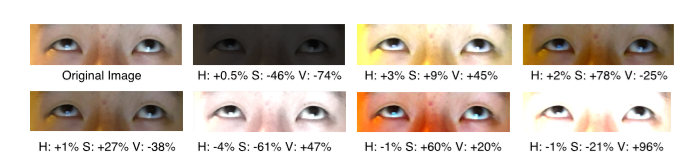
\includegraphics[scale=0.5]{img/yey.png}
    \end{center}
    \caption{Ảnh hưởng sau khi tăng chỉnh sáng}
    \label{refhinh15}
    \end{figure}
\end{center}

%\subsection{Mô hình thuật toán sử dụng}
\textbf{Mô hình thuật toán sử dụng}

\begin{center}
    \begin{figure}[h!]
    \begin{center}
     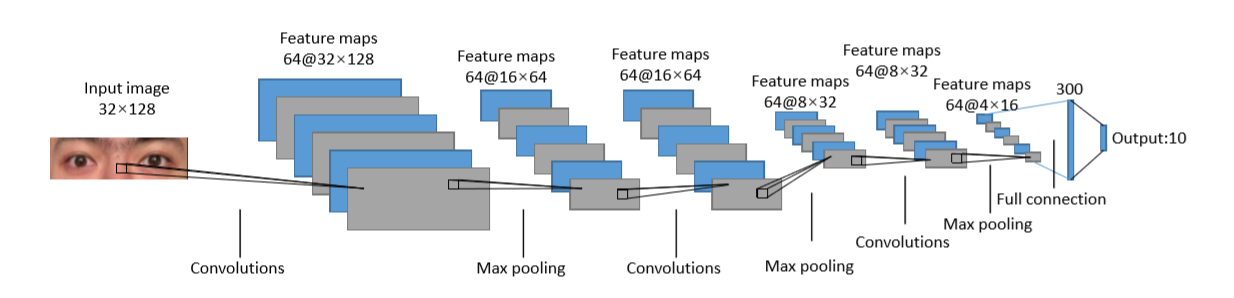
\includegraphics[scale=0.4]{img/yeycnn.png}
    \end{center}
    \caption{Ứng dụng mô hình CNN trong phát hiện hướng nhìn}
    \label{refhinh16}
    \end{figure}
\end{center}

Sử dụng các hình ảnh RGB với kích thước 32 x 128 pixel làm đầu vào mạng. Đối với lớp xoắn (convolution) đầu tiên, kích thước bộ lọc (filter) là 3x3 và bộ lọc (filter) dịch chuyển dọc theo ảnh và quét toàn bộ ảnh. Số lượng các bộ lọc là 64. Sau lớp xoắn, tiếp theo là ReLU và lớp tổng hợp tối đa (max pooling) thu được kích thước 64 x 16 x 64. Lặp lại hoạt động tương tự trên các lớp xoắn thứ hai và thứ ba. Lớp kết nối hoàn chỉnh (full connection) có 300 đơn vị ẩn và mỗi đơn vị có kết nối đến tất cả các bản đồ đặc trưng của lớp xoắn thứ ba. Đầu ra của mạng là mười loại (9 hướng mắt và nháy mắt), sử dụng chức năng softmax để tính toán tối ưu hóa.

\textbf{Kết quả đạt được}

Bảng thống kê dữ liệu thu được sau hai lần nguyên cứu lấy mẫu.

\begin{center}
    \begin{figure}[h!]
    \begin{center}
     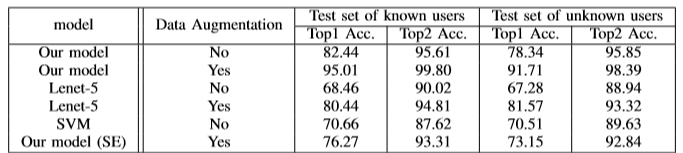
\includegraphics[scale=0.5]{img/table.png}
    \end{center}
    \caption{Bảng thống kê kết quả}
    \label{refhinh17}
    \end{figure}
\end{center}

Nhóm nguyên cứu đã quan sát thấy các hình ảnh ước lượng sai và phát hiện ra hướng sai, ước tính thường gần đúng hướng. Suy luận rằng có thể nguyên nhân ước lượng không chính xác, do người dùng định hướng sai cạnh của hai hướng liền kề. Nếu tính toán lỗi trên lần 2 (đợt lấy mẫu 2), tỷ lệ lỗi sẽ giảm xuống còn 0.2\%. Loại lỗi này có thể chấp nhận được vì khi sử dụng hệ thống để nhập từ (input words), người dùng luôn nhìn vào phần giữa của mọi hướng thay vì nhìn vào cạnh của hướng. Theo kết quả kiểm tra, mô hình với dữ liệu mắt đơn có tỷ lệ lỗi cao hơn. Từ tất cả các dữ liệu mắt người, ước tính sai, tìm thấy ba lý do sau đây: thứ nhất, dữ liệu mắt đơn nhạy cảm hơn với sự chuyển động nhẹ của đầu. Sự nghiêng đầu ảnh hưởng đến kết quả ước tính. Thứ hai, dưới độ phân giải thấp và điều kiện ánh sáng yếu, hình ảnh của mắt đơn có thể quá mờ để sử dụng ước lượng, ngay cả con người không thể nhận ra hướng. Thứ ba, mắt trái và phải không phải lúc nào cũng đồng bộ. Một số hình ảnh kết quả ước lượng của hai mắt là khác nhau nhưng cả hai đều hợp lý.

Để giải quyết những vấn đề tìm thấy, nhóm nguyên cứu đã thiết kế hệ thống bằng cách giải quyết cả vấn đề theo dõi mắt và các vấn đề nhập văn bản, phương pháp nhập văn bản dựa trên thị giác mà người dùng có thể nhập văn bản bằng chuyển động mắt và nhấp nháy, chọn các thanh điện thoại thông thường 9-key T9 bố trí bàn phím như giao diện. Một bộ dữ liệu quy mô lớn đã được thu thập bằng cách sử dụng một số thiết bị chụp và bao gồm các điều kiện ánh sáng khác nhau, địa điểm và thời gian. Sử dụng hình ảnh của cả hai mắt để tránh các vấn đề đồng bộ hóa hình ảnh mắt đơn, làm tăng độ chính xác ước lượng. Đối với các mục đích ứng dụng, xác định 9 hướng đi và học từ một mô hình CNN để đánh giá sự quan sát, có thể chính xác ước tính của người được biết đến (người tham gia lấy mẫu lần 2 trở lên) và người lạ (người tham gia lấy mẫu đầu tiên). Các phương pháp tăng dữ liệu được dùng cung cấp tính mạnh mẽ và tăng độ chính xác ước lượng. Phương pháp nhập văn bản này sử dụng các thiết bị có chi phí thấp, đơn giản hóa các bước hiệu chỉnh và lọc tiếng ồn do đường cong, nháy mắt tự nhiên và ước lượng sai lệch tạm thời trong suốt quá trình hoạt động, ngoài ra có thể chạy ở hai chế độ: chế độ ngoài màn hình và chế độ màn hình. Ở chế độ ngoài màn hình, người dùng có thể tự di chuyển và thiết bị cầm tay. Tốc độ nhập văn bản của chế độ màn hình có thể đạt 20 chữ trong một phút và tắt màn hình chế độ có thể đạt 18 chữ trong một phút với tỷ lệ lỗi thấp. Công việc trong tương lai của nhóm nghiên cứu này là giới thiệu mô hình ngôn ngữ và thêm các chức năng dự đoán và hoàn thành từ cho hệ thống hiện tại và đào tạo ước tính quan sát bất biến.
\section{Appearance-Based Gaze Estimation in the Wild \cite{appearance}}

\textbf{Hướng tiếp cận}

Hình ảnh đầu vào bước đầu được xử lý nhận diện khuôn mặt và điểm 6 điểm mốc (bao  gồm hai điểm của mỗi mắt và hai mốc điểm miệng). Sau đó dùng khuôn mặt 3D chung để ước tính các vị trí 3D của các điểm mốc đã được phát hiện và áp dụng công nghệ kỹ thuật chuẩn hóa không gian để cắt và biến dạng đứng đầu và hình ảnh mắt vào không gian đào tạo bình thường. Bước cuối cùng CNN  được đưa vào để học và đưa ra kết quả dự đoán.
\begin{center}
    \begin{figure}[h!]
    \begin{center}
     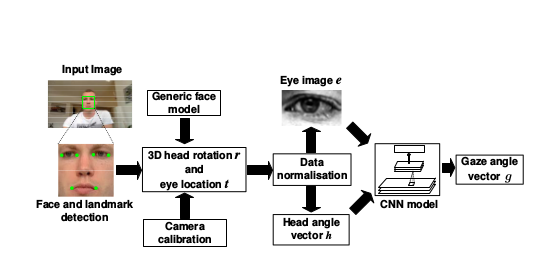
\includegraphics[scale=0.5]{img/h.png}
    \end{center}
    \caption{Xử lý đầu vào}
    \label{refhinh18}
    \end{figure}
\end{center}

\textbf{Mô hình thuật toán sử dụng}

Trong bài báo khoa học này tác giả sử dụng mạng LeNet bao gồm  một mạng tích chập (convolution) - hàm tổng hơp tối đa (max-pooling) - mạng tích chập - hàm tổng hợp tối đa - tầng kết nối đầy đủ (fully - connected). Lớp cuối cùng là một tuyến tính để đưa ra output cuối cùng. Đầu vào là hình ảnh màu xám có kích thước 60x36 pixels. Mỗi tích chập có kích thước feature 5x5 pixels, trong đó số feature của tầng thứ nhất là 20, tầng thứ 2 là 50. Đầu ra là hai góc nhìn, trái và phải.
\begin{center}
    \begin{figure}[h!]
    \begin{center}
     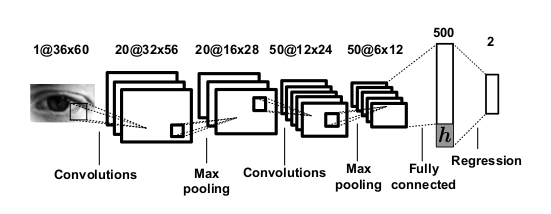
\includegraphics[scale=0.5]{img/conv.png}
    \end{center}
    \caption{Hình ảnh được đưa qua mạng học sâu để xử lý}
    \label{refhinh19}
    \end{figure}
\end{center}
\newpage
\textbf{Kết quả đạt được}

Bảng bên dưới là  sai số trung bình đạt được với môt số mô hình khác. Bao gồm Random Forests (RF), k-Nearest Neighbours(kNN), Adaptive Linear Regression (ALR), Support Vector Regression (SVR).
\begin{center}
    \begin{figure}[h!]
    \begin{center}
     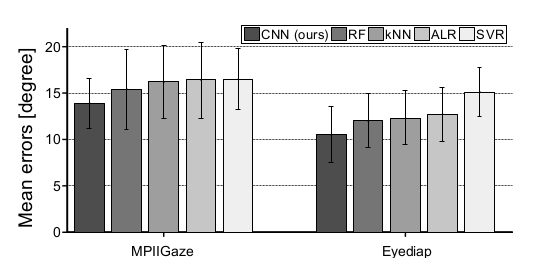
\includegraphics[scale=0.5]{img/2dataset.png}
    \end{center}
    \caption{Bảng thống kê kết quả}
    \label{refhinh20}
    \end{figure}
\end{center}
\section{Rendering of Eyes for Eye-Shape Registration and Gaze Estimation
\cite{eyeShapeRegistrationAndGazeEstimation}}
Nhóm nghiên cứu tạo ra một số lượng lớn hình ảnh thực tế của mắt bằng cách sử dụng mô hình vùng mắt động. Chúng được sử dụng làm dữ liệu đào tạo để đăng ký hình dạng mắt và ước tính dựa trên sự xuất hiện dựa trên sự xuất hiện.
\begin{center}
    \begin{figure}[h!]
    \begin{center}
     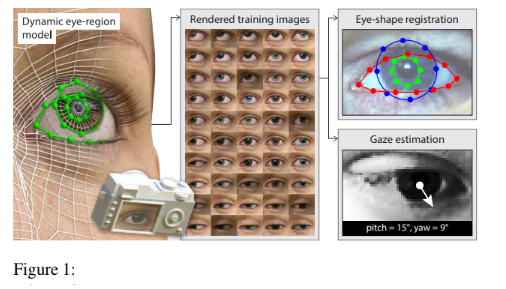
\includegraphics[scale=1]{img/photorealistic_images_of_eyes.png}
    \end{center}
    \caption{Chúng tôi tạo ra một số lượng lớn các hình ảnh photorealistic của mắt bằng cách sử dụng một mô hình vùng mắt động.}
    \label{refhinh20}
    \end{figure}
\end{center}
\textbf{Hướng tiếp cận}

(a) Quét hình ảnh 3D dày đặc (1,4 triệu đa giác (polygons))

(b) Được tái hiện lại thành dạng tối ưu cho hoạt ảnh (9,005 đa giác (polygons))

(c) Các chi tiết bề mặt da có độ phân giải cao được khôi phục bằng bản đồ dịch chuyển 

(d) Các điểm mốc mí mắt và mí mắt 3D được chú giải bằng tay 

(e) Hiển thị mẫu được hiển thị 
\begin{center}
    \begin{figure}[h!]
    \begin{center}
     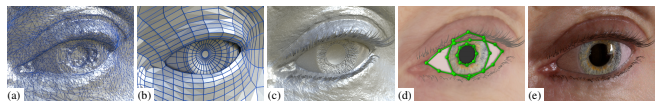
\includegraphics[scale=0.75]{img/An_overview_of_our_model_preparation_process.png}
    \end{center}
    \caption{Tổng quan về quá trình chuẩn bị mô hình.}
    \label{refhinh20}
    \end{figure}
\end{center}
Mô hình mắt nghiên cứu bao gồm các sclera, học sinh, mống mắt, và giác mạc (a) (the sclera, pupil, iris, and cornea) và có thể thể hiện sự thay đổi thực tế trong cả hai hình dạng (giãn nở đồng tử) và kết cấu (màu iris, tĩnh mạch scleral) (b).
\begin{center}
    \begin{figure}[h!]
    \begin{center}
     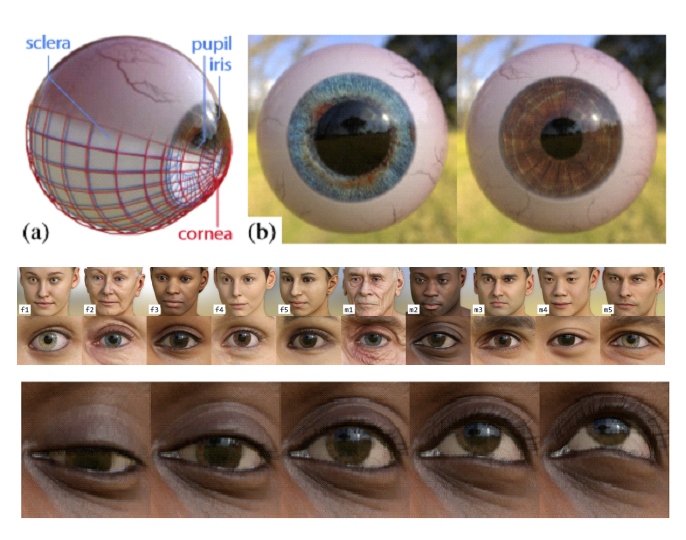
\includegraphics[scale=0.75]{img/Eye_model_and_3D_head_model.png}
    \end{center}
    \caption{Mô hình mắt và mô hình đầu (3D).}
    \label{refhinh20}
    \end{figure}
\end{center}

Máy ảnh được định vị để mô phỏng các thay đổi trong tư thế đầu (a). Tại vị trí này, chúng tôi hiển thị nhiều hình ảnh mắt cho các hướng nhìn khác nhau bằng cách đặt mô hình nhãn cầu (b):
\begin{center}
    \begin{figure}[h!]
    \begin{center}
     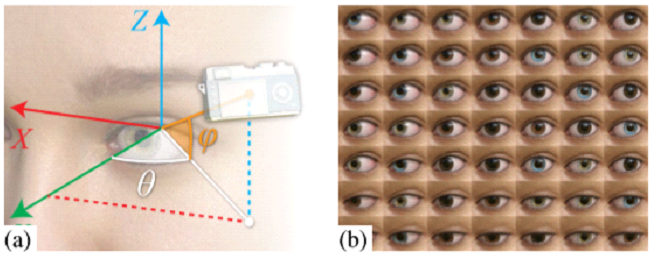
\includegraphics[scale=0.75]{img/Camera_position.png}
    \end{center}
    \caption{Vị trí máy ảnh.}
    \label{refhinh20}
    \end{figure}
\end{center}

Bốn bản đồ môi trường HDR, sử dụng cho ánh sáng thực tế: sáng / ngoài trời nhiều mây và sáng / tối trong nhà. Màu đỏ thể hiện điểm số tồi tệ nhất.

\begin{center}
    \begin{figure}[h!]
    \begin{center}
     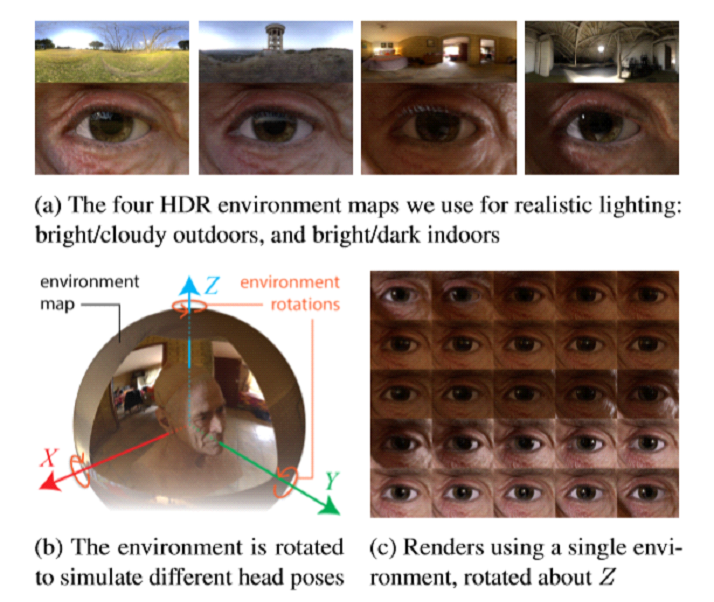
\includegraphics[scale=0.5]{img/Appearance_variation_from_lighting.png}
    \end{center}
    \caption{Sự biến đổi từ việc thay đổi ánh sáng được mô hình hóa với ảnh chụp có môi trường có phạm vi năng động cao.}
    \label{refhinh20}
    \end{figure}
\end{center}

\begin{center}
    \begin{figure}[h!]
    \begin{center}
     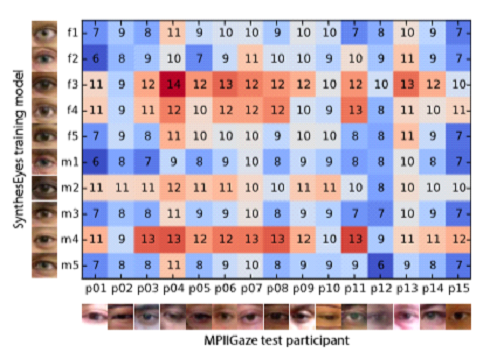
\includegraphics[scale=0.5]{img/Estimation_of_errors_on_MPIIGaze.png}
    \end{center}
    \caption{Ước lượng lỗi trên MPIIGaze}
    \label{refhinh20}
    \end{figure}
\end{center}
Nhóm nghiên cứu đã trình bày một phương pháp mới để tổng hợp những hình ảnh cận cảnh thực tế được dán nhãn hoàn hảo của mắt người. Một đường ống đồ họa máy tính sử dụng một bộ sưu tập các mô hình vùng mắt động thu được từ quét đầu để tạo ra các hình ảnh cho thấy phạm vi của các tư thế đầu, hướng nhìn và điều kiện chiếu sáng. Nhóm nghiên cứu đã chứng minh rằng phương pháp nghiên cứu hoạt động tốt hơn các phương pháp hiện đại để đăng ký hình dạng mắt và ước tính dựa trên sự xuất hiện dựa trên dữ liệu chéo trong tự nhiên. Những kết quả này hứa hẹn và nhấn mạnh tiềm năng quan trọng của các phương pháp tổng hợp học tập như vậy, đặc biệt là sự bứt phá với các phương pháp giám sát quy mô lớn gần đây.
\textbf{Kết quả đạt được}
Ví dụ về độ phù hợp (fits) với SynthesEyes eye-CLNF về hình ảnh trong tự nhiên (a) và hình ảnh webcam (b). Hai hàng hình ảnh trên cùng minh họa cho việc nhận dạng hình dạng mắt thành công, trong khi hàng dưới cùng minh họa các trường hợp thất bại, bao gồm các vệt chưa được tạo ra (tóc), các tư thế chưa được chỉnh sửa (mắt kín), kính và khởi tạo mô hình không chính xác.
\begin{center}
    \begin{figure}[h!]
    \begin{center}
     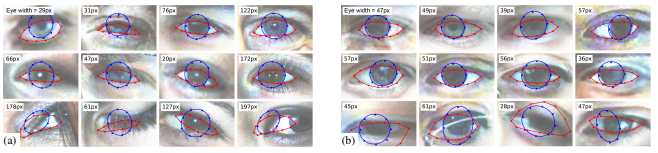
\includegraphics[scale=0.75]{img/Example_fits_of_our_SynthesEyes_eye_CLNF.png}
    \end{center}
    \caption{Ví dụ về độ phù hợp (fits) với SynthesEyes eye-CLNF}
    \label{refhinh20}
    \end{figure}
\end{center}
Trục x đại diện cho tập huấn luyện được sử dụng. Dấu chấm là các lỗi trung bình và đường màu đỏ thể hiện một giới hạn thấp hơn về mặt xác thực (số điểm xác thực chéo trong tập dữ liệu).

\begin{center}
    \begin{figure}[h!]
    \begin{center}
     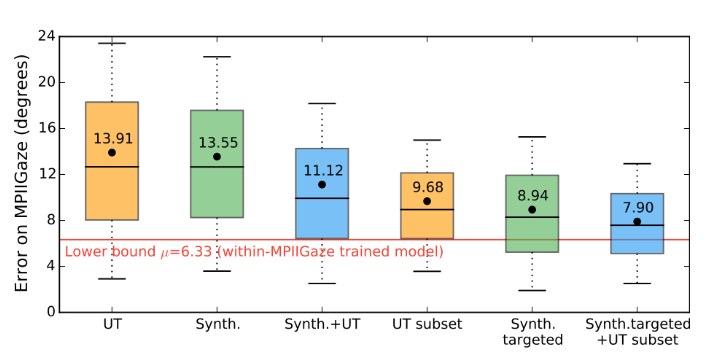
\includegraphics[scale=0.70]{img/Performance_chart_on_MPIIGaze.png}
    \end{center}
    \caption{Biểu đồ hiệu suất trên MPIIGaze}
    \label{refhinh15}
    \end{figure}
\end{center}

\section{Learning an appearance-based gaze estimator from one million synthesised images \cite{Learninganappearancebasedgazeestimator}}

\textbf{Hướng tiếp cận}

Nghiên cứu đã cung cấp một triệu hình ảnh thực tế về mắt bằng cách sử dụng mô hình vùng mắt được mô phỏng. Chúng được kết hợp với một hình ảnh đầu vào bằng cách sử dụng một phương pháp tiếp cận hàng xóm gần nhất (nearest-neighbor approach) để ước lượng cái nhìn. Mô hình quản lý này tìm ra các kết quả phù hợp ngay cả với các góc nhìn cực độ và ánh sáng chói từ kính.

\begin{center}
    \begin{figure}[h!]
    \begin{center}
     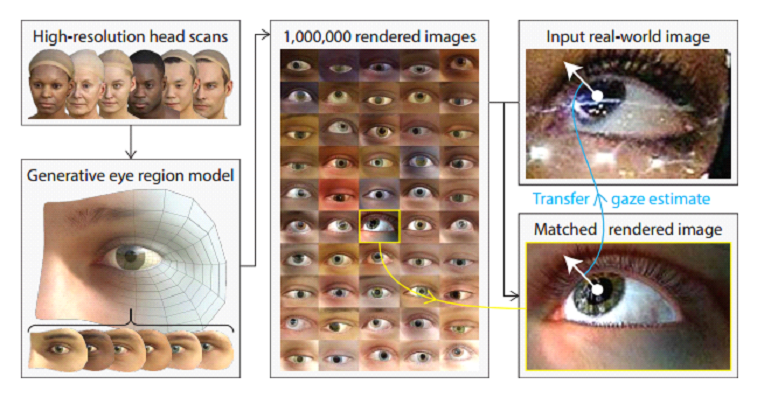
\includegraphics[scale=0.70]{img/Image_dataset_the_nearest_neighbor_approach.png}
    \end{center}
    \caption{Sử dụng phương pháp tiếp cận hàng xóm gần nhất(nearest-neighbor approach) để ước lượng cái nhìn.}
    \label{refhinh15}
    \end{figure}
\end{center}

Nhóm nghiên cứu trình bày về UnityEyes, một phương pháp mới để tổng hợp nhanh chóng số lượng lớn các hình ảnh vùng mắt thay đổi cho dữ liệu huấn luyện. Phương pháp nghiên cứu này: kết hợp một mô hình 3D sinh học mới lạ của vùng mắt người với khung thời gian thực. Mô hình vùng mắt có nguồn gốc từ quét khuôn mặt 3D có độ phân giải cao và sử dụng xấp xỉ thời gian thực cho các vật liệu và cấu trúc nhãn cầu phức tạp, cũng như các phương pháp hình học thủ tục lấy cảm hứng từ giải phẫu cho hoạt ảnh mí mắt. Tổng hợp hình ảnh bằng cách sử dụng trình kết xuất đồ họa và ánh sáng dựa trên hình ảnh thực tế và đa dạng điều kiện chiếu sáng. Những hình ảnh tổng hợp này có thể được khớp với hình ảnh đầu vào trong thế giới thực bằng cách sử dụng các phương pháp tiếp cận gần nhất để ước lượng ánh mắt. 

\begin{center}
    \begin{figure}[h!]
    \begin{center}
     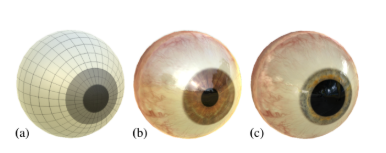
\includegraphics[scale=1]{img/Eyeball_mesh.png}
    \end{center}
    \caption{Hình ảnh về lưới mắt: (a) được hiển thị với các vật liệu dựa trên vật lý và các hiệu ứng khúc xạ, mô hình co rút đồng tử (b) và giãn nở (c).}
    \label{refhinh15}
    \end{figure}
\end{center}

\begin{center}
    \begin{figure}[h!]
    \begin{center}
     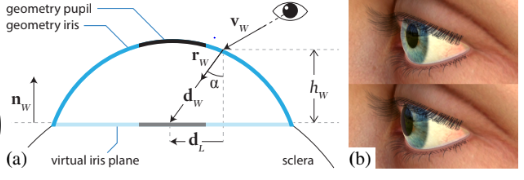
\includegraphics[scale=1]{img/Model_iris_refraction.png}
    \end{center}
    \caption{Mô hình khúc xạ iris bằng cách thay đổi kết cấu tra cứu: Một điểm ảnh được xem khúc xạ chính xác để hiển thị màu đen (tròng mắt) thay vì màu xanh (bề mặt hình học).}
    \label{refhinh15}
    \end{figure}
\end{center}

\begin{center}
    \begin{figure}[h!]
    \begin{center}
     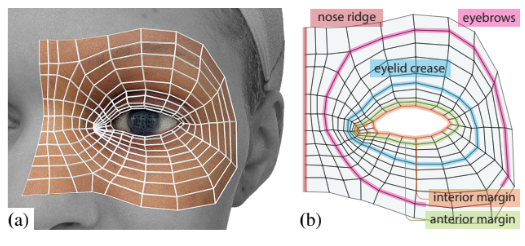
\includegraphics[scale=1]{img/Generative_eye_region_model.PNG}
    \end{center}
    \caption{Mô hình khởi tạo vùng mắt: (a) Cho thấy cấu trúc liên kết vùng mắt chung của chúng ta (229 đỉnh) trên một quét thô (khoảng 5M đỉnh). (b) Cho thấy cấu trúc liên kết trong không gian kết cấu uv với các vòng cạnh quan trọng được đánh dấu.}
    \label{refhinh15}
    \end{figure}
\end{center}

\textbf{Kết quả đạt được}

Nearest-neighbour pairs hiển thị hình ảnh tự nhiên (trên cùng) và phần kết của chúng tôi (dưới cùng) cùng với ánh mắt được ước tính (màu xanh lá cây).
Ba hàng đầu hiển thị ước tính chất lượng tốt, ngay cả dưới ánh sáng khó khăn (thiếu ánh sáng), độ phân giải thấp và góc nhìn cực đoan.
Hàng dưới cùng hiển thị các trường hợp lỗi từ biến thể chưa được sửa đổi, ví dụ: trang điểm và tóc.

\begin{center}
    \begin{figure}[h!]
    \begin{center}
     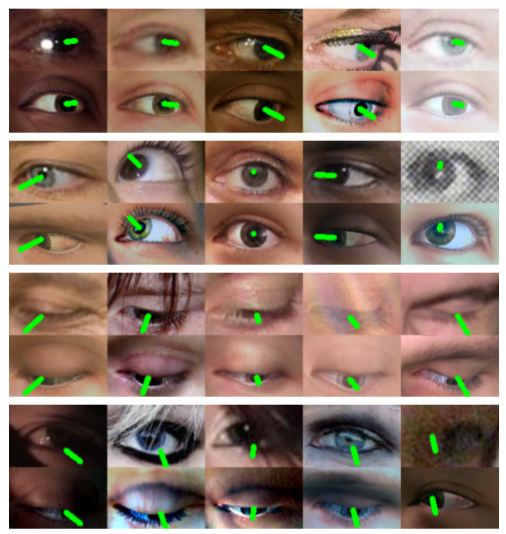
\includegraphics[scale=0.7]{img/The_result_of_Nearest_neighbour_pairs.png}
    \end{center}
    \caption{Kết quả của phương pháp tổng hợp những hình ảnh cận cảnh thực tế (Nearest-neighbour pairs) được dán nhãn hoàn hảo của mắt người }
    \label{refhinh15}
    \end{figure}
\end{center}

Lỗi pixel và điểm nhìn của phương pháp nearest-neighbor tương ứng với tập UnityEyes và MPIIGaze. Nhóm nguyên cứu đạt được lỗi thấp nhất ở 1.4 triệu hình ảnh.


\begin{center}
    \begin{figure}[h!]
    \begin{center}
     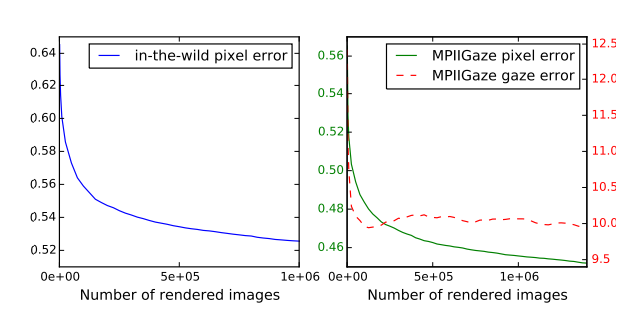
\includegraphics[scale=1]{img/Pixel_and_gaze_errors_for_nearest_neighbor.png}
    \end{center}
    \caption{Lỗi pixel và điểm nhìn của phương pháp nearest-neighbor tương ứng với tập UnityEyes và MPIIGaze. Nhóm nguyên cứu đạt được lỗi thấp nhất ở 1.4 triệu hình ảnh.}
    \label{refhinh15}
    \end{figure}
\end{center}


\newpage




\chapter{Kiến thức nền tảng}

\section{Học tăng cường (Reinforcement Learning)}
\subsection{Giới thiệu}
Học tăng cường (Reinforcement Learning) \cite{reinforcementlearninganintroduction} là học cách ánh xạ các tình huống thành hành động để cực đại phần thưởng. Người học không được cho biết hành động nào cần thực hiện, nhưng thay vào đó phải khám phá ra hành động nào mang lại nhiều phần thưởng nhất bằng cách thử chúng. Trong những trường hợp thú vị và khó khăn nhất, các hành động có thể không chỉ ảnh hưởng đến phần thưởng mà còn ảnh hưởng đến tình huống tiếp theo và thông qua đó, cũng ảnh hưởng đến tất cả các phần thưởng tiếp theo. Hai đặc điểm này — tìm kiếm thử-và-sửa sai (trial-and-error) và trì hoãn phần thưởng — là hai đặc điểm phân biệt quan trọng nhất của học tăng cường.

\subsection{Các thành phần của học tăng cường}
Ngoài \textit{agent} (tác nhân) và \textit{environment} (môi trường), người ta có thể xác định bốn thành phần chính của hệ thống học tăng cường: \textit{policy} (chính sách), \textit{reward signal} (tín hiệu phần thưởng), \textit{value function} (hàm giá trị), và có thể có thêm \textit{model} (mô hình) của môi trường.

\begin{itemize}
    \item \textbf{Policy:} xác định cách hoạt động của tác nhân tại một thời điểm nhất định. Nói một cách đại khái, một \textit{policy} là một ánh xạ từ các trạng thái nhận thức của môi trường đến các hành động sẽ được thực hiện khi ở trong các trạng thái đó. Nó tương ứng với những gì trong tâm lý học sẽ được gọi là một tập hợp các quy tắc hoặc liên kết kích thích-phản ứng. Trong một số trường hợp, \textit{policy} có thể là một hàm hoặc bảng tra cứu đơn giản, trong khi trong những trường hợp khác, \textit{policy} có thể liên quan đến tính toán mở rộng chẳng hạn như quá trình tìm kiếm. \textit{Policy} là cốt lõi của một tác nhân học tăng cường theo nghĩa là chỉ nó là đủ để xác định hành vi. Nói chung, các \textit{policy} có thể ngẫu nhiên, chỉ rõ xác suất cho mỗi hành động.
    \item \textbf{Reward signal:} xác định mục tiêu trong vấn đề học tăng cường. Trên mỗi bước thời gian, môi trường gửi cho tác nhân một số duy nhất được gọi là phần thưởng. Mục tiêu duy nhất của tác nhân là tối đa hóa tổng phần thưởng mà tác nhân nhận được trong thời gian dài. Do đó, \textit{reward signal} xác định đâu là những sự kiện tốt và xấu đối với tác nhân. Trong một hệ thống sinh học, chúng ta có thể nghĩ về phần thưởng tương tự như trải nghiệm của niềm vui hoặc nỗi đau. Chúng là các đặc điểm tức thời và xác định vấn đề mà tác nhân phải đối mặt. \textit{Reward signal} là cơ sở chính để thay đổi \textit{policy}; nếu một hành động được \textit{policy} chọn theo sau là \textit{reward} thấp, thì \textit{policy} có thể được thay đổi để chọn một số hành động khác trong tình huống đó trong tương lai. Nói chung, các \textit{reward signal} có thể là các hàm ngẫu nhiên của trạng thái môi trường và các hành động được thực hiện.
    \item \textbf{Value function:} Trong khi \textit{reward signal} cho biết điều gì tốt theo nghĩa tức thời, thì một \textit{value function} chỉ định điều gì tốt về lâu dài. Nói một cách đại khái, \textit{value} của một trạng thái là tổng số phần thưởng mà một tác nhân có thể mong đợi tích lũy trong tương lai, bắt đầu từ trạng thái đó. Trong khi \textit{reward} xác định mong muốn ngay lập tức, nội tại của các trạng thái môi trường, thì các \textit{value} cho thấy mong muốn lâu dài của các trạng thái sau khi tính đến các trạng thái có khả năng tuân theo và \textit{reward} có sẵn trong các trạng thái đó. Ví dụ: một trạng thái có thể luôn mang lại \textit{reward} tức thì thấp nhưng vẫn có \textit{value} cao vì nó thường xuyên được theo sau bởi các trạng thái khác mang lại \textit{reward} cao. Hoặc điều ngược lại có thể đúng. Để so sánh giữa con người với con người, \textit{reward} có phần giống như niềm vui (nếu cao) và nỗi đau (nếu thấp), trong khi \textit{value} tương ứng với sự đánh giá tinh tế hơn và có tầm nhìn xa hơn về mức độ hài lòng hoặc không hài lòng của chúng ta khi môi trường của chúng ta đang ở trong một trạng thái cụ thể.
    \item \textbf{Model environment:} Đây là thứ bắt chước hành vi của môi trường, hay nói chung hơn, cho phép đưa ra các suy luận về cách môi trường sẽ hoạt động. Ví dụ: với một trạng thái và hành động, mô hình có thể dự đoán trạng thái kết quả tiếp theo và phần thưởng tiếp theo. Mô hình được sử dụng để lập kế hoạch, theo đó chúng ta có thể quyết định một quá trình hành động bằng cách xem xét các tình huống có thể xảy ra trong tương lai trước khi chúng thực sự trải qua.
\end{itemize}

\subsection{Ứng dụng của học tăng cường}
Do tính chất của việc học tăng cường là luôn tối ưu việc đạt được phần thưởng cuối cùng dựa vào trạng thái, và phần thưởng hiện tại, cùng với sự tác động của môi trường nên việc học tăng cường được áp dụng nhiều trong các lĩnh vực mang đậm tính tương tác lâu dài giữa tác nhân và môi trường, có thể kể đến:

\begin{itemize}
    \item Điều khiển xe tự hành, robot, v.v.
    \item Các hệ thống gợi ý (Recommendation System), hỏi đáp (Chatbot), v.v.
    \item Ngành công nghiệp trò chơi (game) như là cờ vây (nổi tiếng với AlphaGo), v.v.
\end{itemize}

Cụ thể, trong luận án này sẽ sử dụng phương pháp học tăng cường cho việc huấn luyện mô hình tư vấn khách hàng.

\section{Hệ thống Chatbot hướng mục tiêu (Goal Oriented Chatbot)}
\subsection{Chatbot hướng mục tiêu}
\label{subsec:chatbotgo}
Yêu cầu của một hệ thống tư vấn khách hàng là ta phải đặt cho nó một ngữ cảnh (tư vấn cái gì) và mục tiêu cuối cùng cần hoàn thành khi tư vấn. Vì vậy, đây là một bài toán hướng mục tiêu.

Một Chatbot hướng mục tiêu (GO) cố gắng giải quyết một vấn đề cụ thể cho người dùng. Các Chatbot này có thể giúp mọi người đặt vé, tìm đặt chỗ, v.v. Có hai cách chính để huấn luyện một Chatbot GO: Học có giám sát (supervised learning) với bộ mã hóa-giải mã (encoder-decoder), ánh xạ trực tiếp cuộc đối thoại của người dùng tới phản hồi và học tăng cường giúp huấn luyện một Chatbot thông qua các cuộc hội thoại thử-và-sửa sai (trial-and-error) với người dùng thực hoặc trình mô phỏng người dùng có quy tắc.

Như đã nói từ phần trước, luận án này sử dụng mô hình học tăng cường vì các tối đa lợi thế của nó.

\subsection{Kiến trúc tổng quát của hệ thống Chatbot GO}
Hệ thống đối thoại cho một Chatbot GO sử dụng phương pháp học tăng cường được chia thành 3 phần chính, được mô tả như hình \ref{fig:chatbot}: Phần Quản lý hội thoại (Dialogue Manager), phần Hiểu ngôn ngữ tự nhiên (Natural Language Understanding) và phần Trình tạo ngôn ngữ tự nhiên (Natural Language Generator). Phần Quản lý hội thoại được chia thành Bộ theo dõi trạng thái hội thoại (Dialogue State Tracker) và \textit{policy} cho chính tác nhân, được đại diện bởi mạng nơ-ron (neural network) trong nhiều trường hợp. Ngoài ra, vòng lặp hệ thống chứa một người dùng với các mục tiêu. Mục tiêu người dùng thể hiện những gì người dùng muốn để thoát khỏi cuộc trò chuyện.

\begin{center}
    \begin{figure}[h!]
        \begin{center}
         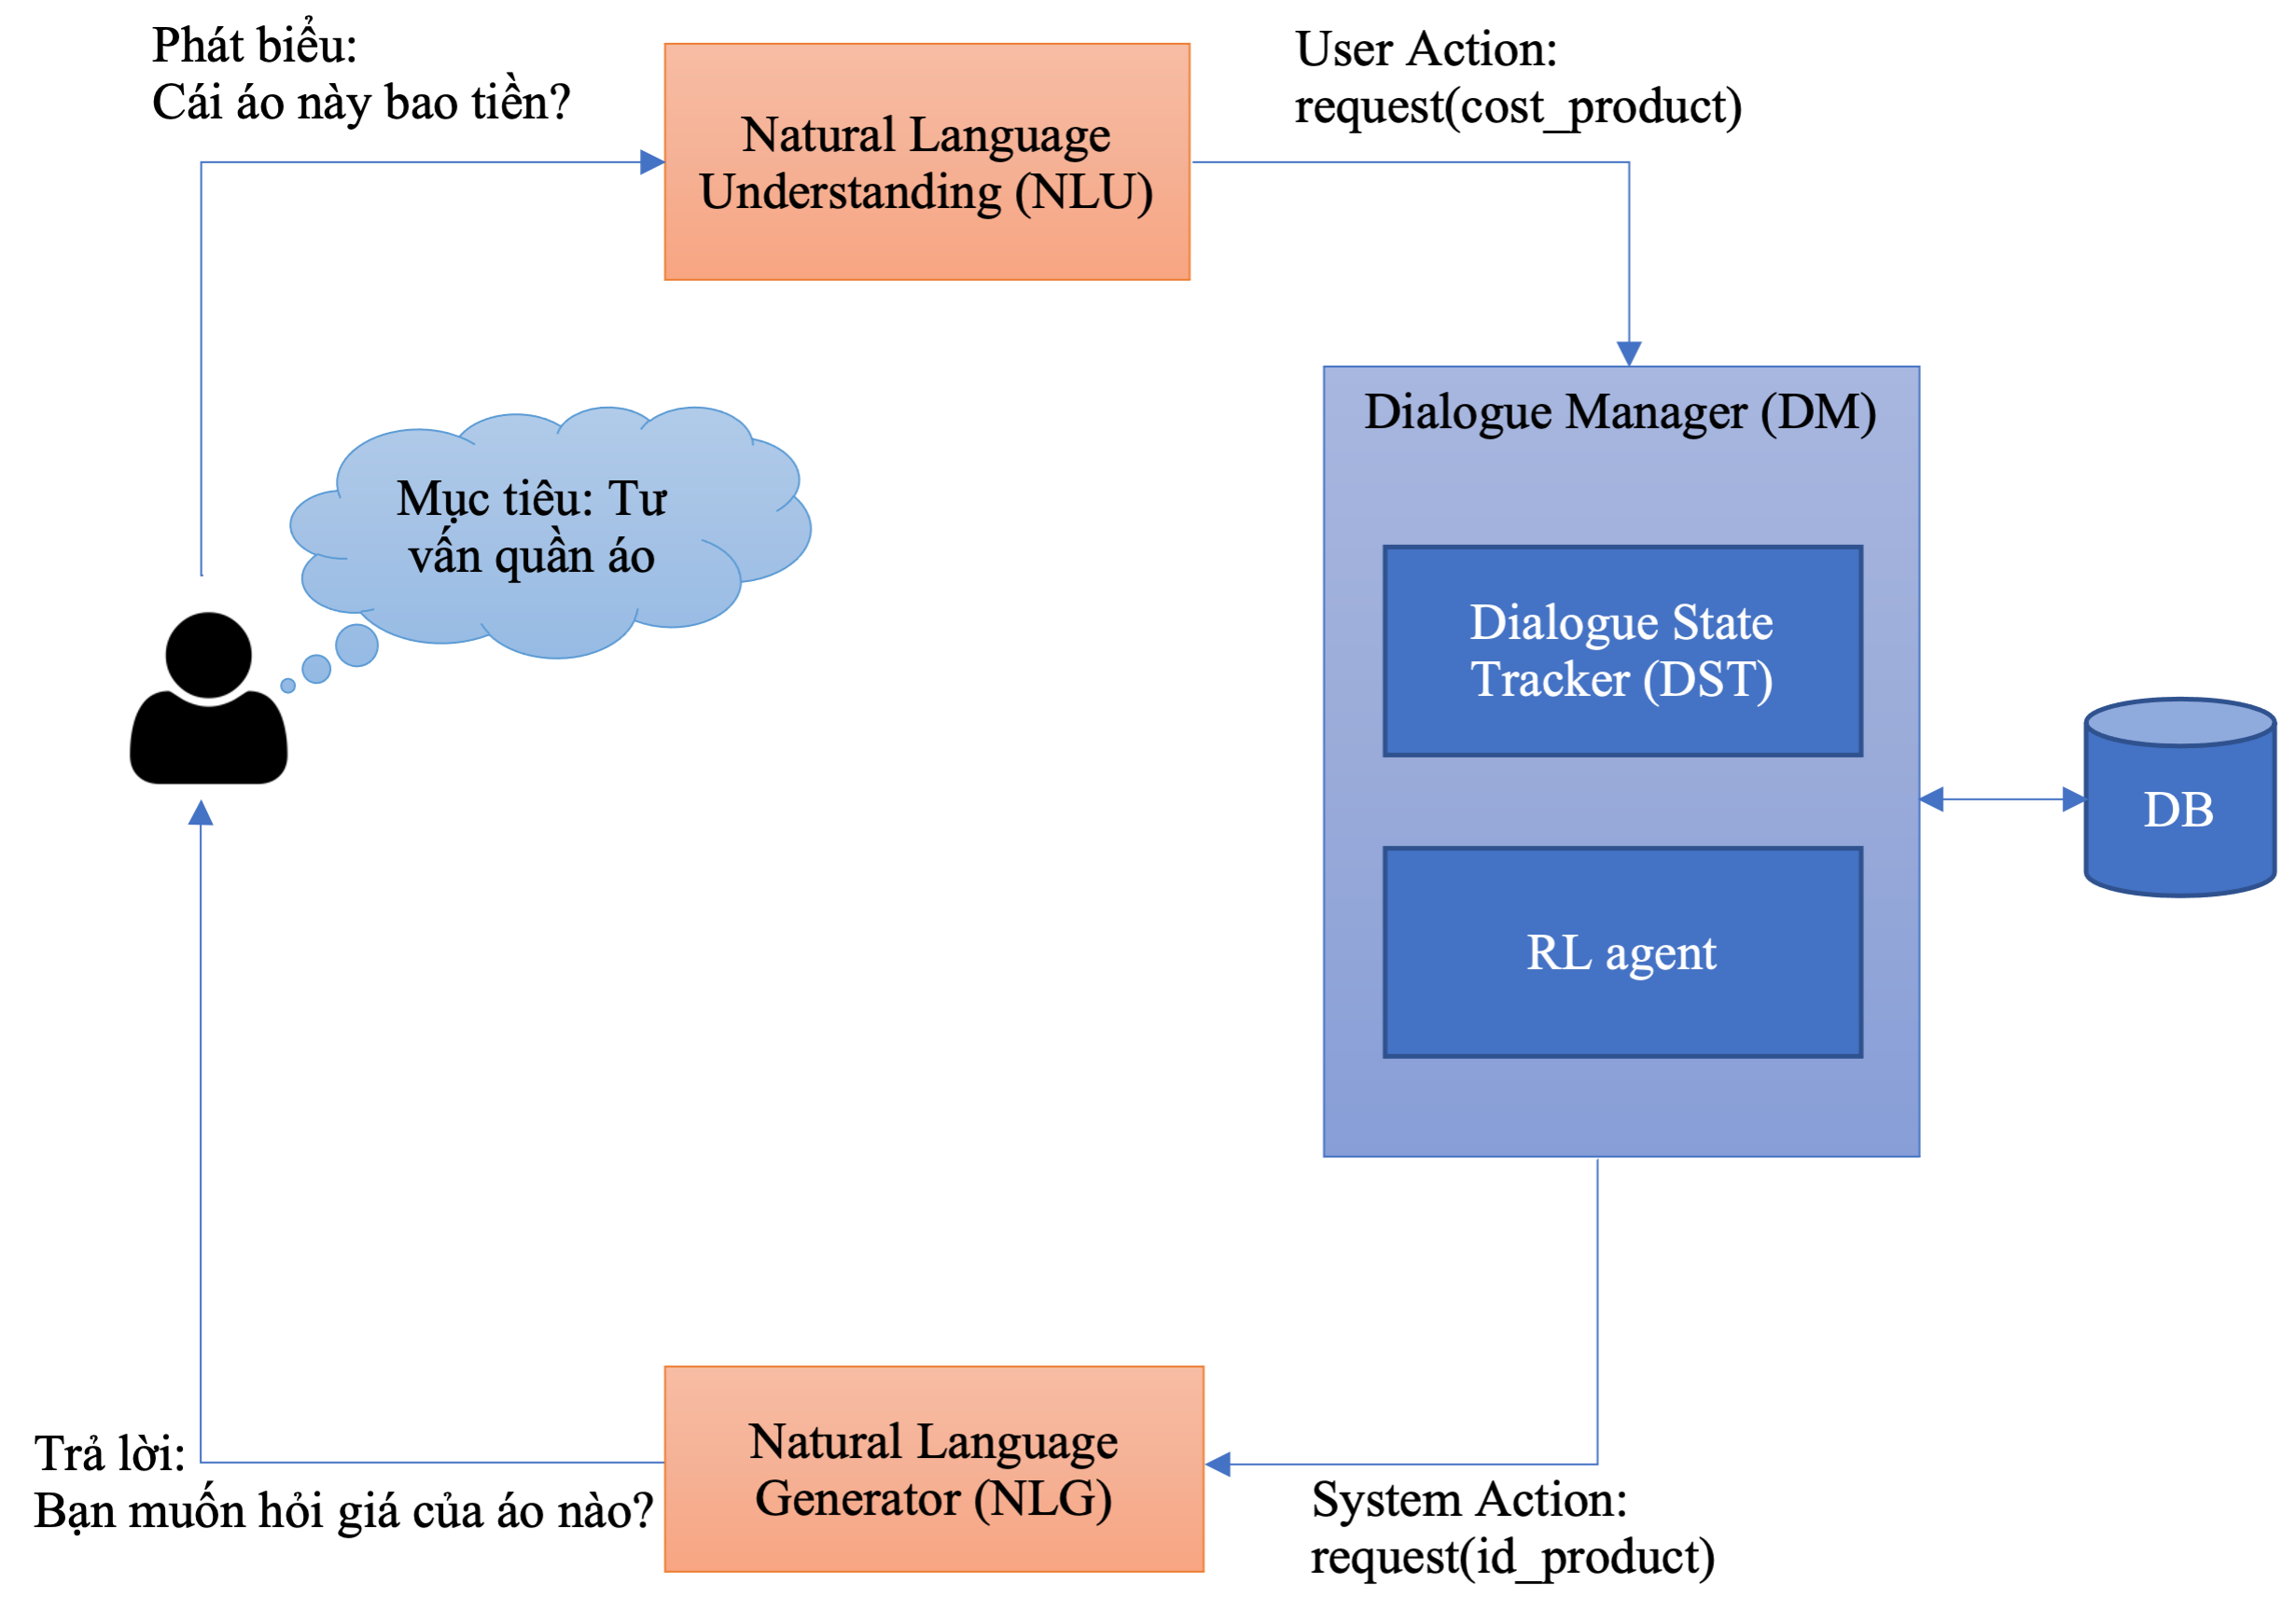
\includegraphics[scale=0.8]{chapter3/img/overviewchatbot.png}
        \end{center}
        \caption{Kiến trúc tổng quát của mô hình Chatbot GO sử dụng phương pháp học tăng cường}
        \label{fig:chatbot}
    \end{figure}
\end{center}

Khi người dùng gửi đi một thông điệp (Cái áo này bao tiền?), sẽ được xử lý bởi thành phần Hiểu ngôn ngữ tự nhiên (NLU), chuyển ngôn ngữ tự nhiên thành một dạng mà tác nhân có thể xử lý, đầu ra (output) là ở dạng khung ngữ nghĩa (semantic frame) (request(cost\_product)).

Sau đó, Bộ theo dõi trạng thái đối thoại (DST) từ hành động của người dùng (đã được chuyển thành khung ngữ nghĩa) và lịch sử của cuộc trò chuyện hiện tại sẽ xử lý và chuyển thành một biểu diễn trạng thái mà có thể xử lý được bởi \textit{policy} của tác nhân. Trạng thái này là đầu vào của \textit{policy} hoặc mạng nơ ron của tác nhân, đầu ra là hành động của tác nhân dưới dạng khung ngữ nghĩa (request(id\_product)).

Cơ sở dữ liệu được truy vấn để thêm thông tin vào cho tác nhân như thông tin các kích thước, màu sắc v.v.

Hành động của tác nhân sau đó được xử lý bởi phần Trình tạo ngôn ngữ tự nhiên (NLG), chuyển nó sang ngôn ngữ tự nhiên để người dùng có thể dễ dàng đọc hiểu (Bạn muốn hỏi giá của áo nào?).

\section{Mô hình học tăng cường cho Chatbot GO}
\label{sec:model}
Như đã đề cập ở mục giới hạn của đề tài \ref{sec:scope}, chúng ta sẽ quan tâm sử dụng mô hình học tăng cường như thế nào để áp dụng vào bài toán hướng mục tiêu tư vấn khách hàng. Trình bày ở mục \ref{subsec:chatbotgo}, một tác nhân Chatbot hướng mục tiêu (GO) sẽ được huấn luyện để trò chuyện thành thạo với người dùng thực nhằm hoàn thành mục tiêu, phù hợp với các ràng buộc của người dùng. Quá trình tác nhân học tập theo phương pháp học tăng cường được mô tả rõ hơn ở hình \ref{fig:learningflow}.

\begin{center}
    \begin{figure}[h!]
        \begin{center}
         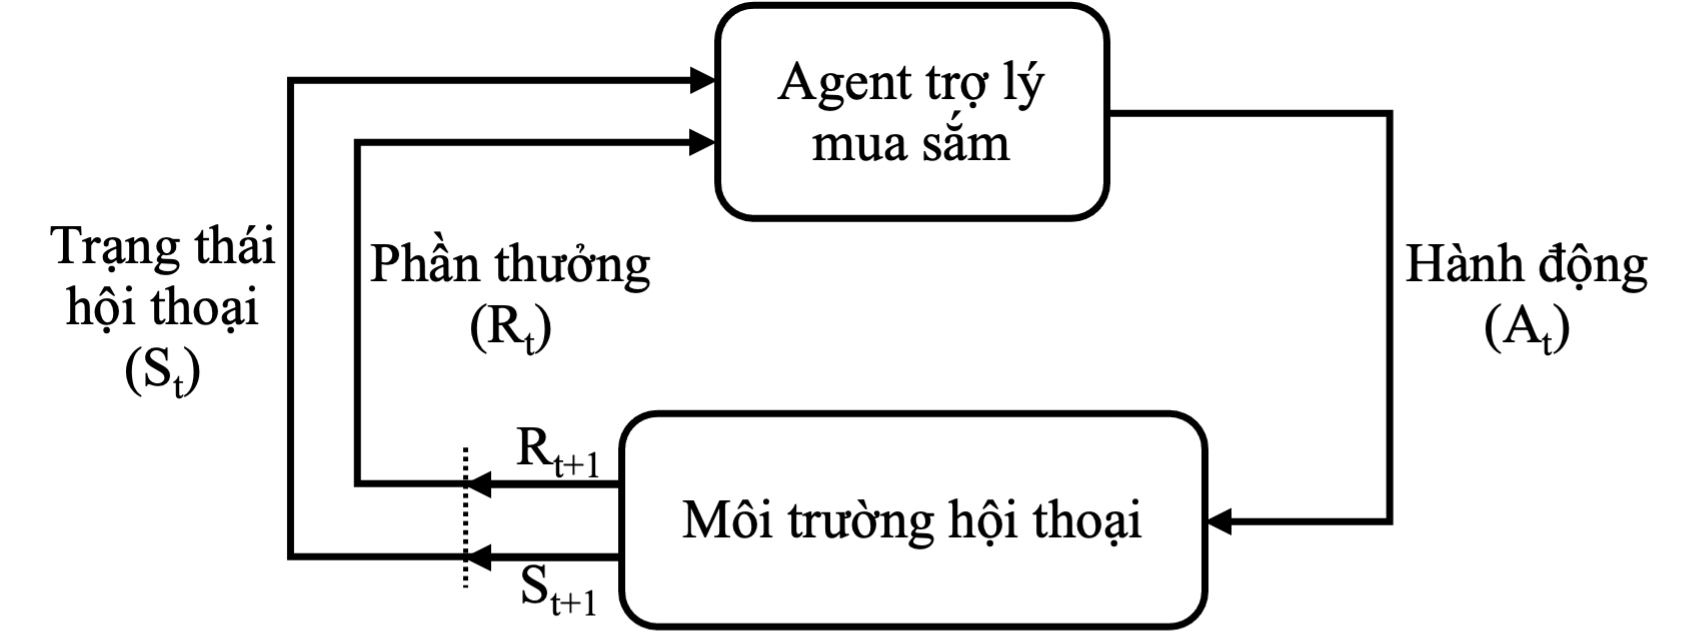
\includegraphics[scale=1]{chapter3/img/learningflow.png}
        \end{center}
        \caption{Quá trình huấn luyện theo phương pháp học tăng cường}
        \label{fig:learningflow}
    \end{figure}
\end{center}

Bản chất của học tăng cường là thử và sửa sai, nó sẽ thử đi thử lại các hành động và rút ra kinh nghiệm sau mỗi lần thử. Trong bài toán tư vấn khách hàng, việc thử này sẽ được thực hiện như sau:

\begin{itemize}
    \item Tại trạng thái hiện tại là $S_t$, tác nhân ngẫu nhiên hoặc theo một luật (policy) nào đó có sẵn chọn ra một hành động $A_t$.
    \item Hành động này sẽ tác động vào môi trường là diễn biến của hội thoại hiện tại cho ra trạng thái mới là $S_{t+1}$ và nhận giá trị là phần thường $R_t$ cho hành động đó.
    \item Phần thưởng này sẽ đánh giá được việc chọn hành động đó có tốt hay không. Từ đó tác nhân cập nhật lại cách chọn hành động.
\end{itemize}

Với mô hình này, ta dễ thấy tác nhân sẽ chỉ nhận đầu vào là trạng thái hội thoại hiện tại để ra quyết định hành động. Vì vậy, ta cần xem xét đến các thông tin cần có trong trạng thái như thế nào để tác nhân có đủ thông tin để ra quyết định. Việc này được trình bày rõ hơn trong mục \ref{subsec:state}.

Trong thời gian đầu, tác nhân có thể ngẫu nhiên chọn các hành động hoặc theo một luật định sẵn đơn giản. Sau đó, nó cần được chỉ ra hành động nào là không tốt, để cập nhập cách chọn hành động (policy), cách thức thực hiện là thông qua điểm thưởng. Các điểm thưởng sẽ được định nghĩa sao cho giống với các yêu cầu của người dùng thật để quá trình tự học của tác nhân là hiệu quả và thỏa mãn với nhu cầu người dùng. Cụ thể được mô tả trong mục \ref{subsec:reward}.

\subsection{Trạng thái hội thoại}
\label{subsec:state}
Trạng thái hội thoại chứa những thông tin hữu ích từ lịch sử hội thoại cho tới thời điểm hiện tại. Các thông tin này có thể khác nhau tùy vào mục đích sử dụng tác nhân. Tuy nhiên, nó nên chứa các thông tin biểu thị tình trạng, những diễn biến đã, đang diễn ra trong hội thoại. Dưới đây diễn giải một số thông tin trong trạng thái hội thoại cho tác nhân trợ lý mua sắm.

Giả sử, ta có một cuộc hội thoại giữa người dùng và cửa hàng diễn ra như sau:

\renewcommand{\lstlistingname}{Ví dụ}
\begin{lstlisting}[caption={Một mẫu đoạn hội thoại},label={exam:dialog1},language=exam_vn,firstnumber=1]
User: Hi shop
Admin: Chào bạn, bạn cần shop tư vấn sản phẩm nào ạ?
User: Chân váy hoa có size gì vậy bạn
Admin: Dạ chân váy hoa bên em có size M, và L ạ
User: Còn màu hồng ko?
Admin: Dạ sản phẩm còn 2 cái ạ
User: OK shop. Mình lấy cái này nha.
Admin: Bạn mặc size gì ạ?
\end{lstlisting}

Tại dòng 3, người dùng hỏi kích thước của sản phẩm. Để tác nhân có thể thực hiện được hành vi đúng là cung cấp thông tin thì nó cần biết rằng yêu cầu hiện tại của người dùng là gì (yêu cầu thông tin kích thước) và thông tin người dùng cung cấp (tên sản phẩm). Vì vậy, trạng thái hội thoại cần chứa hành động hiện tại của người dùng.

Tại dòng 5, người dùng yêu cầu thông tin số lượng và cung cấp thông tin màu sắc. Tuy nhiên, ta biết rằng để tìm kiếm đúng sản phẩm phù hợp, cần biết tên của sản phẩm. Mà tên sản phẩm đã được người dùng cung cấp tại dòng 3. Vì vậy, ngoài hành động hiện tại, trạng thái hội thoại còn chứa tất cả các thông tin mà người dùng đã thông báo trước đó.

Tại dòng 7, người dùng muốn đặt đơn hàng. Để chốt được đơn hàng, cửa hàng cần biết đầy đủ thông tin cần thiết của sản phẩm để tìm thấy một mẫu sản phẩm duy nhất. Như ví dụ trên, chân váy hoa có 2 loại kích cỡ khác nhau. Tác nhân cần yêu cầu người dùng cung cấp thêm thông tin này. Vì vậy trong trạng thái hội thoại cần có kết quả sau khi truy vấn cơ sở dữ liệu của từng thông tin.

Ngoài ra, ta cần có thêm hành động gần nhất của tác nhân để tránh việc lặp lại hành động từ tác nhân. Trong nhu cầu thực tế, việc tư vấn và giúp người dùng đạt mục tiêu cuối cùng nên diễn ra nhanh nhất có thể. Vì vậy, số lượt hội thoại đã diễn ra cũng được thêm vào.

\subsection{Phần thưởng và ảnh hưởng của nó đến quyết định hành động}
\label{subsec:reward}
Ta cần định nghĩa phần thưởng phù hợp cho hành động của tác nhân trong mỗi trạng thái hội thoại khác nhau. Xét ví dụ \ref{exam:dialog1}, ta có thể định nghĩa một số điểm thưởng dựa trên phản hồi của người dùng như sau:

\begin{itemize}
    \item Tại dòng 2, hành động của tác nhân đơn giản là chào hỏi lại người dùng. Hành động này thông thường và phản hồi của người dùng là tiếp nối cuộc trò chuyện. Vì vậy, hành động này có thể xem là hành động qua lượt, không mang giá trị điểm thưởng.
    \item Tại dòng 4, tác nhân cung cấp thông tin mà người dùng yêu cầu từ câu trước, hành động này không bị từ chối bởi người dùng ở câu sau. Vì vậy, hành động này xem là cung cấp giá trị có ích cho người dùng và được 1 điểm thưởng.
\end{itemize}

Sau khi có điểm thưởng cho từng hành động, việc tác nhân cập nhật cách chọn hành động và đưa ra hành động mới như thế nào, ta xét ví dụ sau như hình \ref{fig:dialog2}.

\begin{center}
    \begin{figure}[h!]
        \begin{center}
         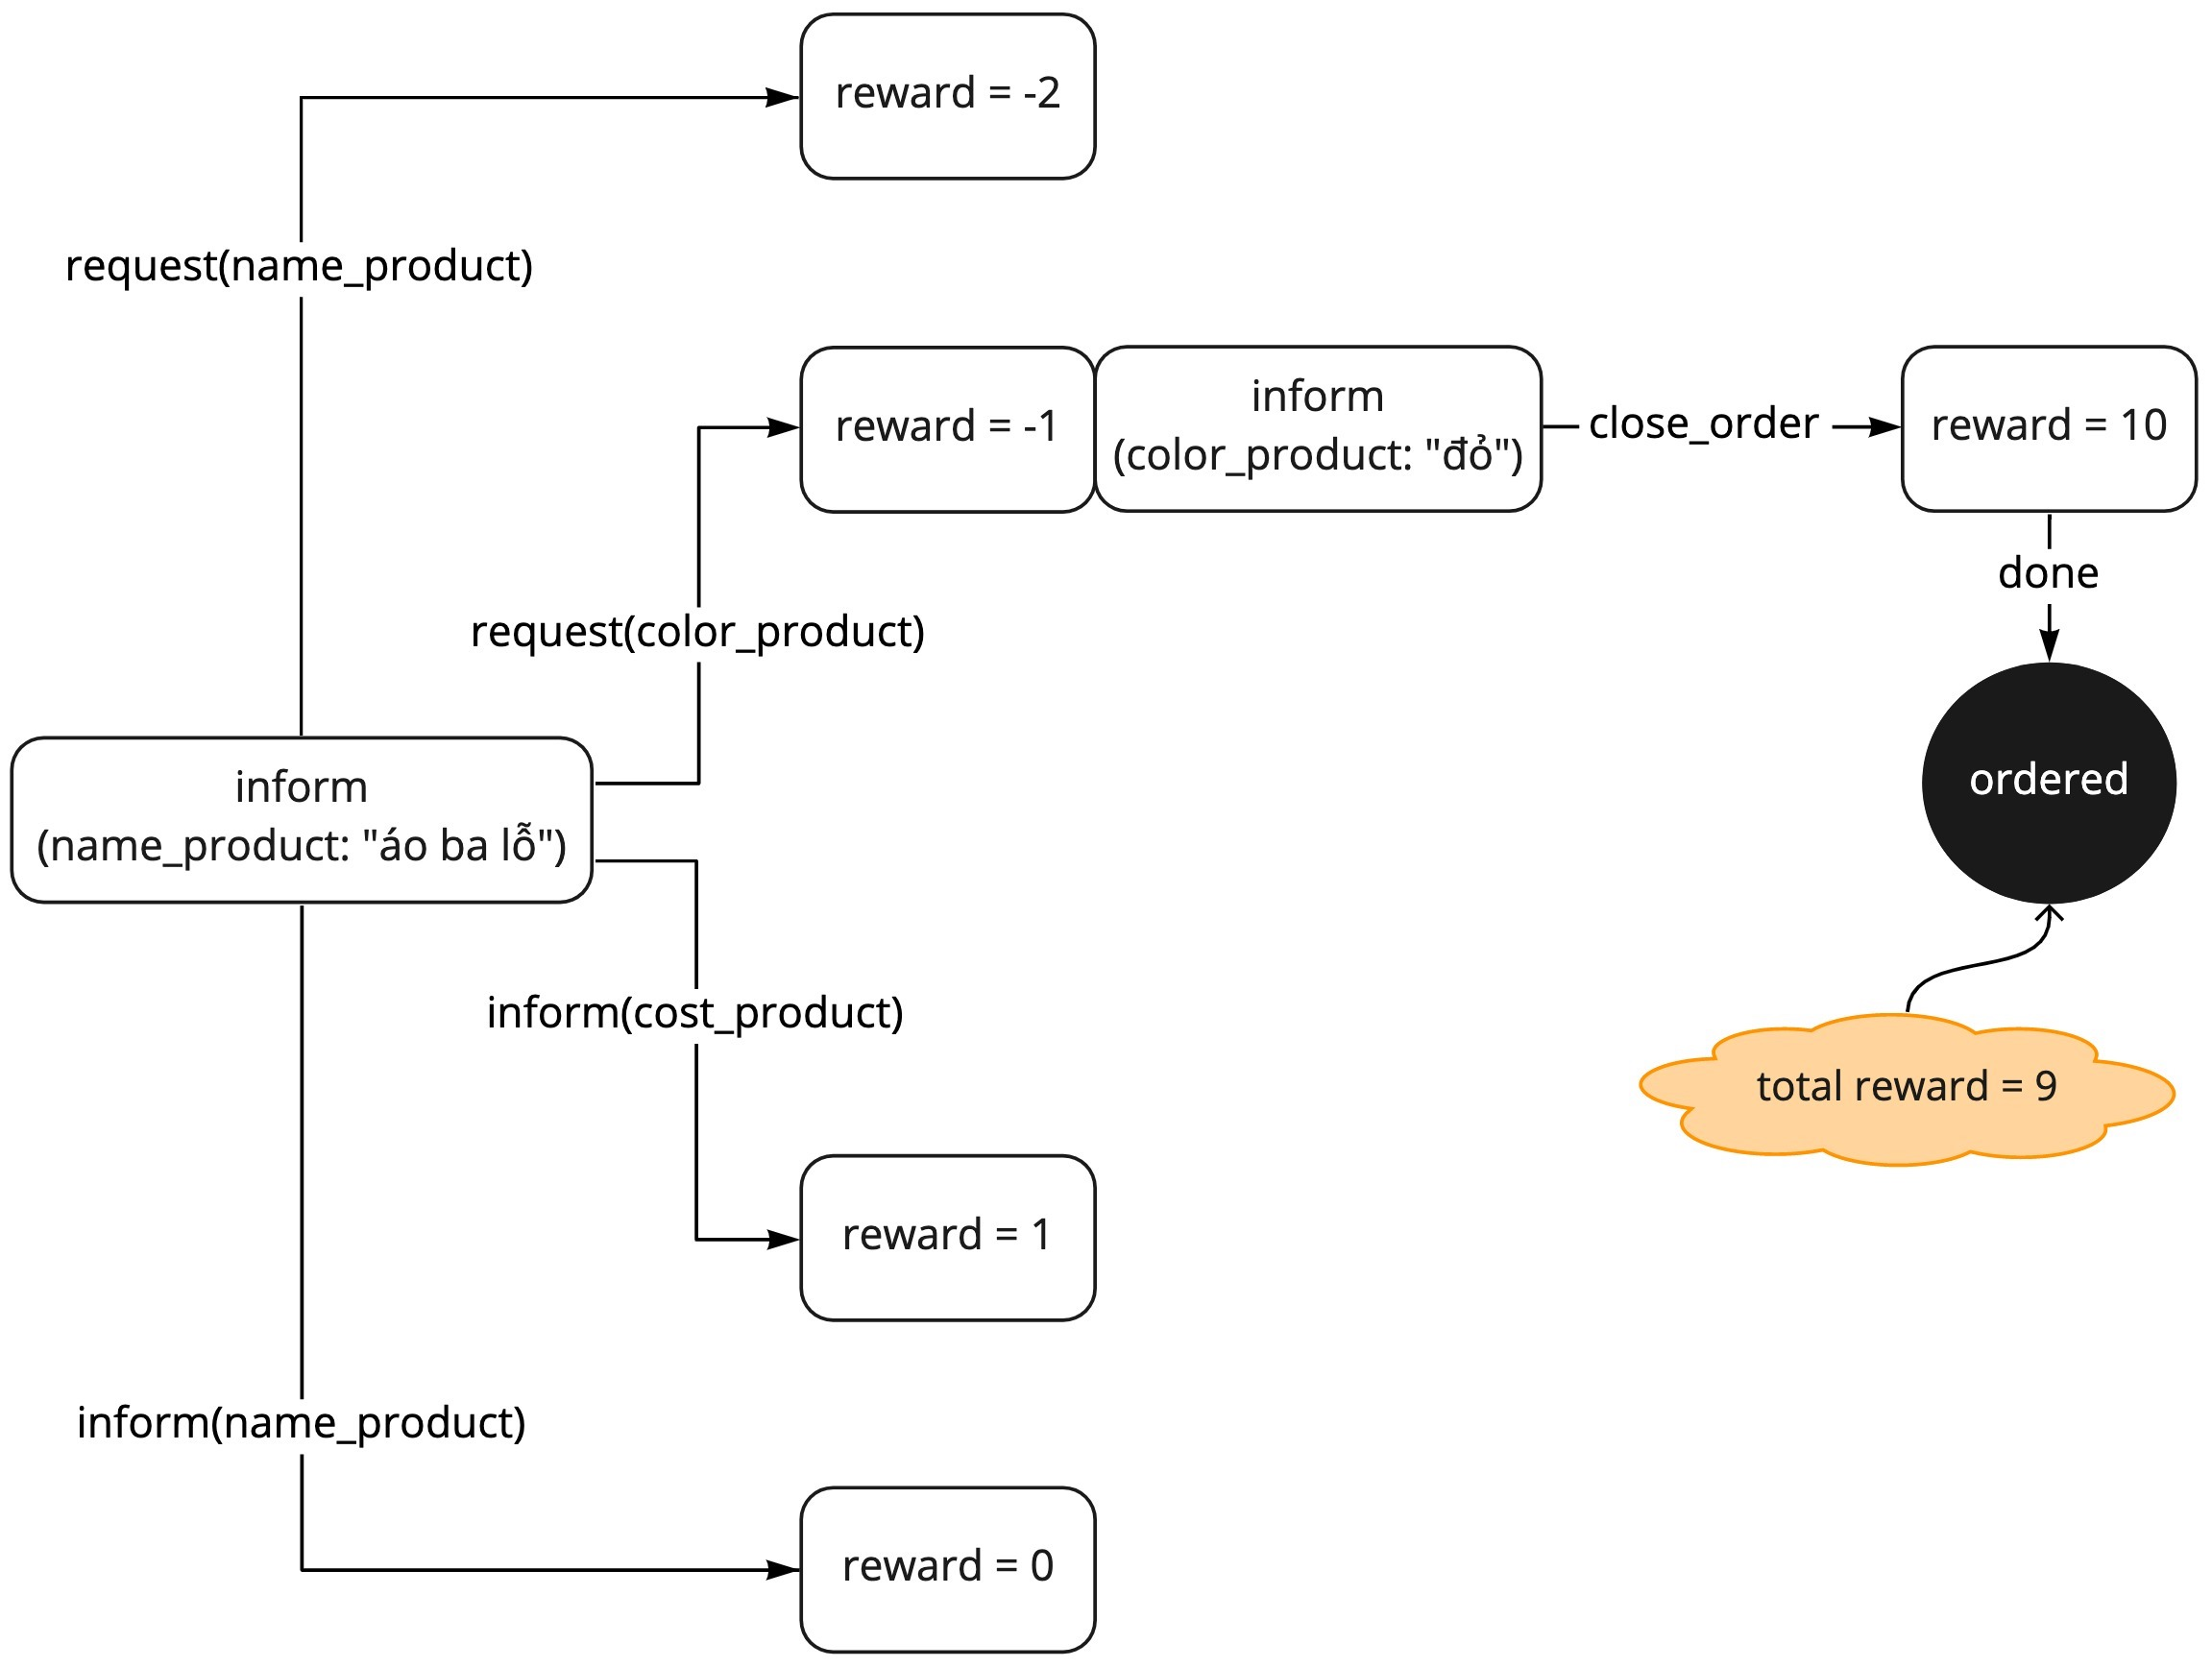
\includegraphics[scale=0.18]{chapter3/img/dialog_ex13.jpg}
        \end{center}
        \caption{Quá trình cho điểm thưởng và ra hành động - phương án 1}
        \label{fig:dialog2}
    \end{figure}
\end{center}

Ta có, quá trình một hội thoại với mục tiêu là chốt đơn hàng. Đầu tiên, người dùng cung cấp thông tin tên sản phẩm (áo ba lỗ). Và tác nhân có các hành động có thể có như sau:

\begin{itemize}
    \item Yêu cầu tên sản phẩm: người dùng đã cung cấp tên sản phẩm trước đó. Vì vậy, đây là hành vi không đúng, gây phiền nhiễu khó chịu cho người dùng. Nó nhận điểm trừ 2.
    \item Yêu cầu thông tin màu sắc: màu sắc là thông tin chưa được cung cấp, tuy nhiên đây là hành vi yêu cầu, không cung cấp thông tin hữu ích cho người dùng. Nó nhận điểm trừ 1.
    \item Thông báo giá sản phẩm: đây là hành vi cung cấp thông tin hữu ích. Nó nhận điểm thưởng 1.
    \item Thông báo tên sản phẩm: người dùng đã cung cấp tên sản phẩm trước đó. Vì vậy, đây là hành vi không cần thiết. Không nhận điểm thưởng nào.
\end{itemize}

Vì mục tiêu của hội thoại này là chốt đơn hàng. Và trong thực tế, ta cần biết đủ thông tin sản phẩm để có được một mẫu hàng duy nhất. Với sản phẩm này có nhiều màu, tác nhân cần yêu cầu người dùng cung cấp thông tin màu sắc sản phẩm mà họ muốn. Sau khi có được thông tin này, nó sẽ hoàn thành được mục tiêu hội thoại với hành động chốt đơn hàng và nhận được điểm thưởng 10. Với luồng hội thoại này, ta nhận được tổng phần thưởng là 9. Qua ví dụ này, ta thấy rằng để hoàn thành được mục tiêu cuối cùng của người dùng, ngoài việc xét điểm thưởng ở mỗi hành động, ta còn phải quan tâm đến phần thưởng của cả cuộc hội thoại.

Xét một trường hợp khác như hình \ref{fig:dialog3}.

\begin{center}
    \begin{figure}[h!]
        \begin{center}
         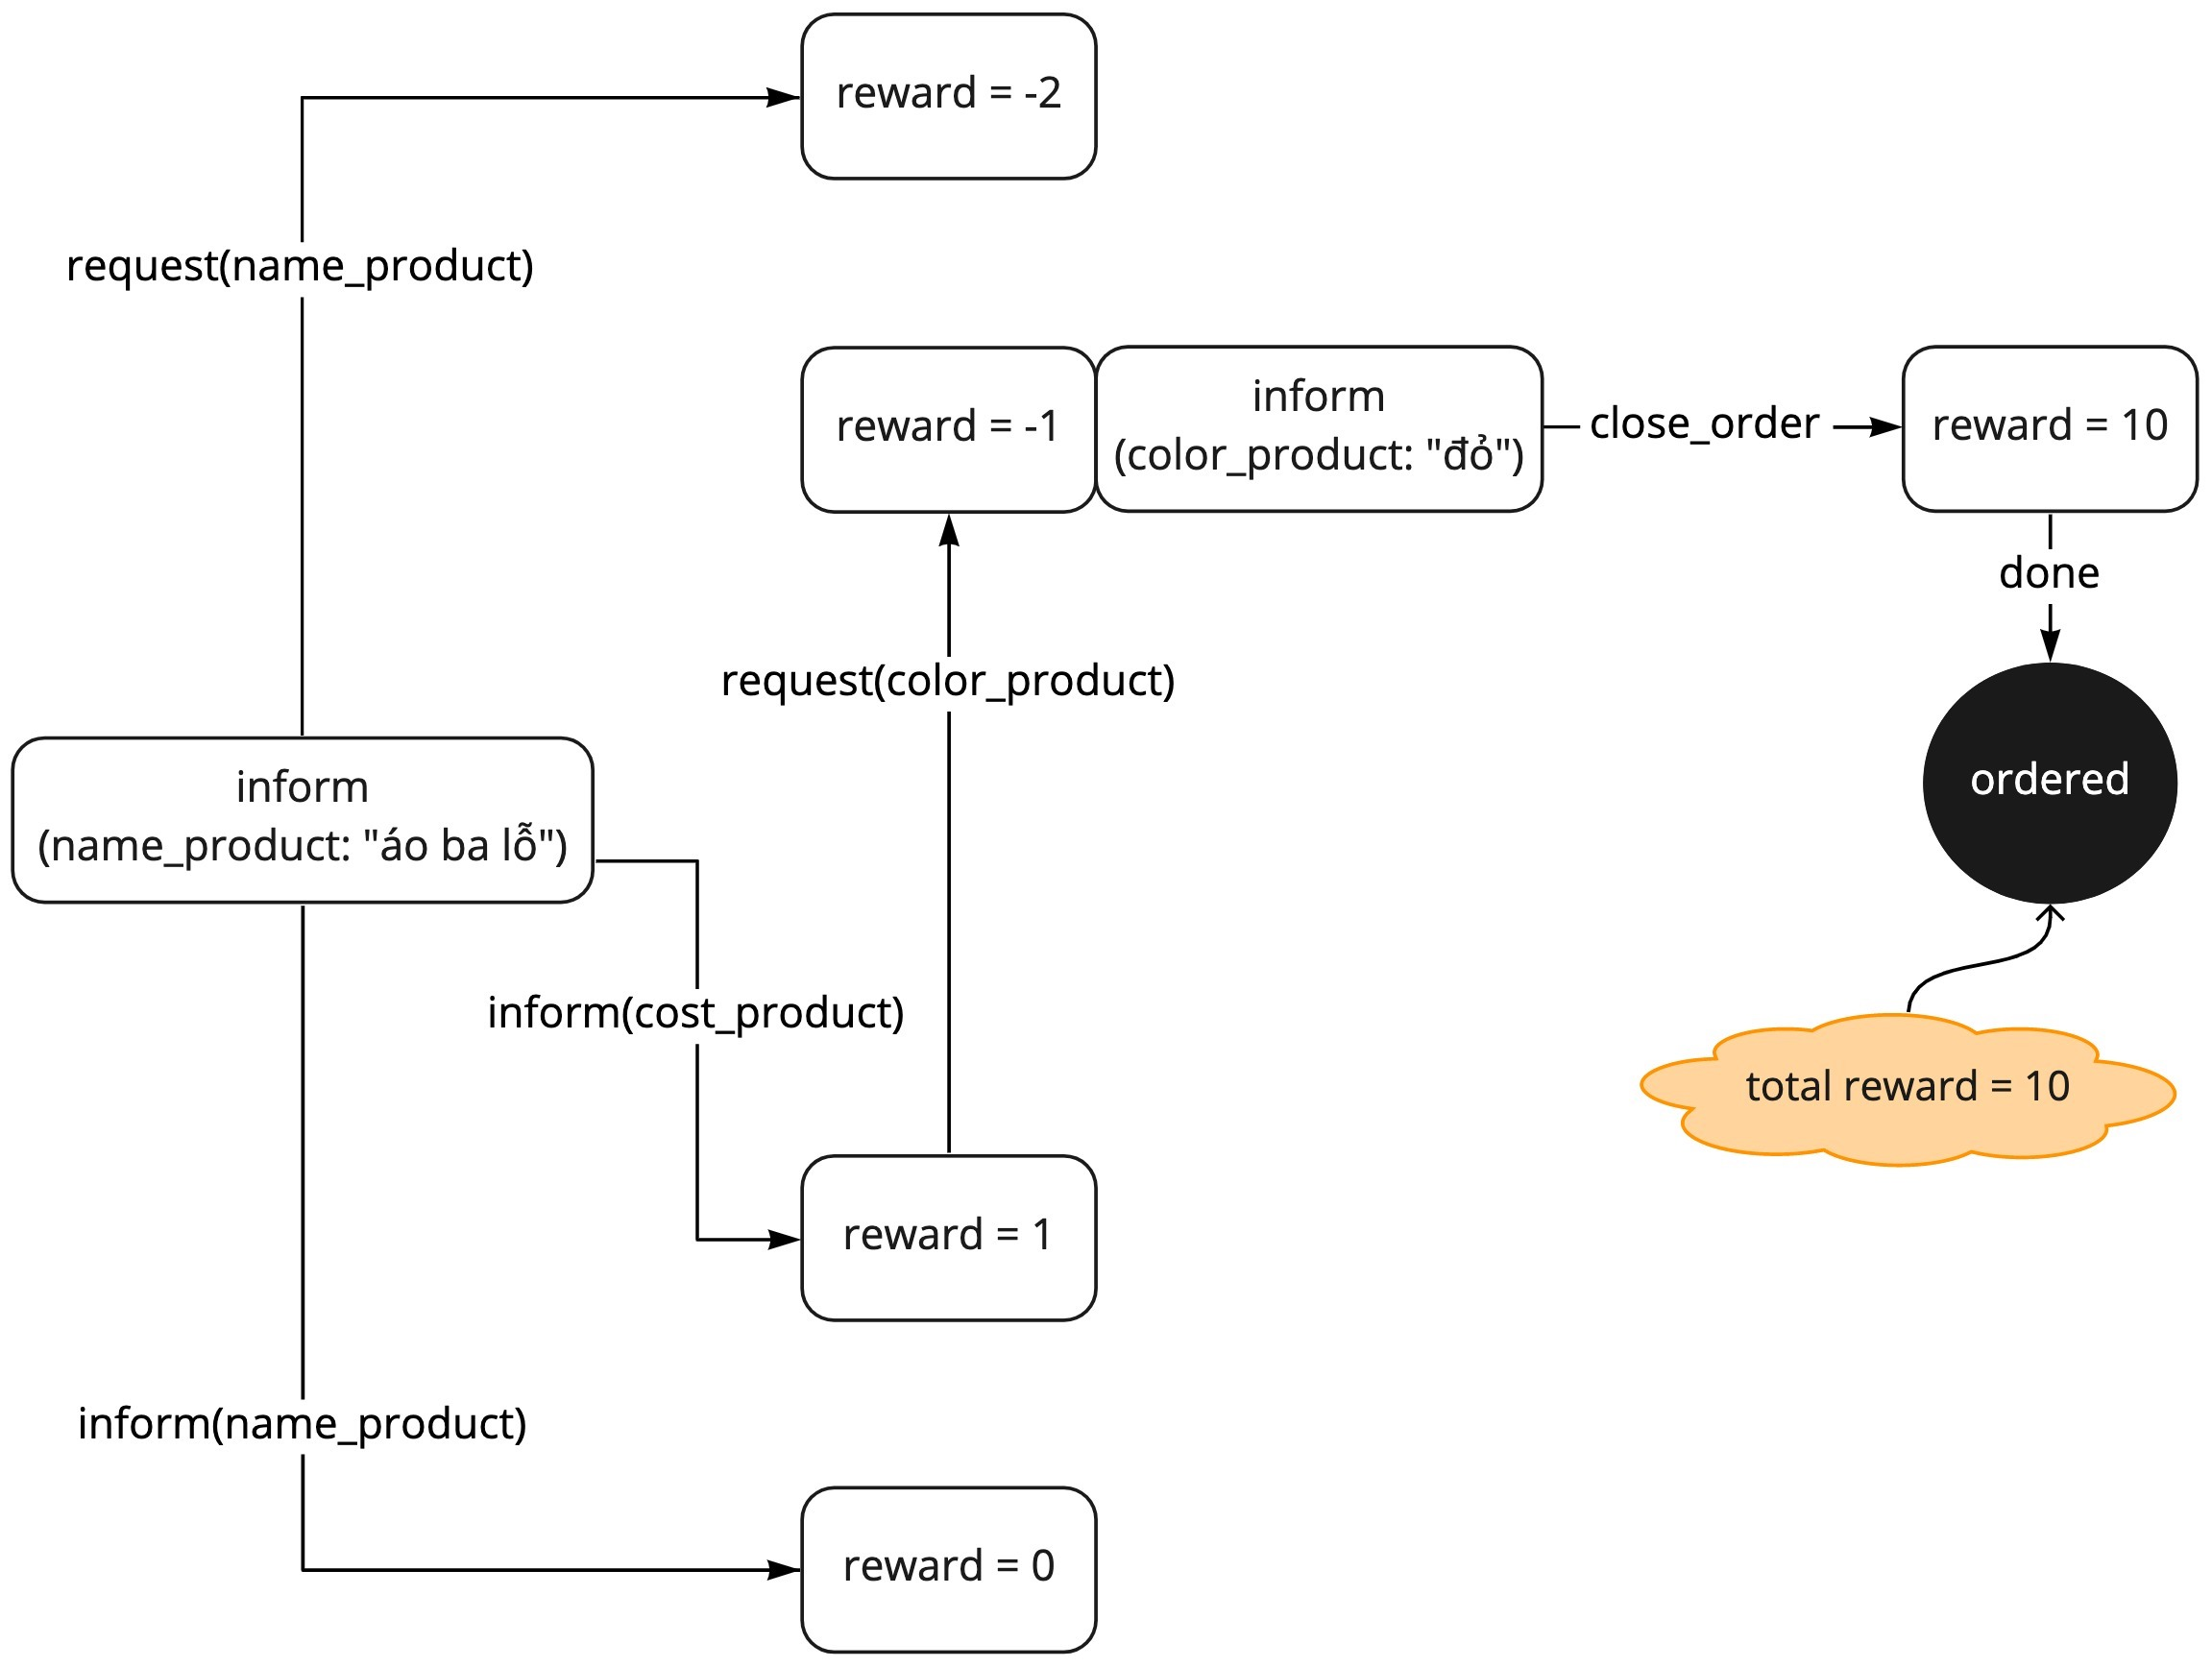
\includegraphics[scale=0.18]{chapter3/img/dialog_ex15.jpg}
        \end{center}
        \caption{Quá trình cho điểm thưởng và ra hành động - phương án 2}
        \label{fig:dialog3}
    \end{figure}
\end{center}

Thay vì ngay lập tức yêu cầu thông tin màu sắc, tác nhân có thể thông báo một thông tin hữu ích là giá đơn hàng, nhận được phần thưởng là 1. Mặc dù, nó không được yêu cầu bởi người dùng. Khi đó, tổng phần thưởng nhận được có giá trị là 10, cao hơn trường hợp lúc nãy. Tuy nhiên, như đã biết, ta mong đợi tác nhân hoàn thành mục tiêu cho người dùng nhanh nhất có thể. Hạn chế các hành động không cần thiết. Vì vậy, ngoài điểm thưởng cho từng hành động, quá trình tính tổng điểm thưởng, còn kèm theo một tham số, gọi là gamma ($\gamma$). Tham số này nhỏ hơn 1. Với mỗi điểm thưởng cho từng hành động sẽ được nhân với lũy thừa của gamma. Với bậc là số lượt hội thoại đã thực hiện cho đến hiện tại. Việc này sẽ làm giảm giá trị tổng điểm thưởng khi tác nhân càng đi nhiều bước (thực hiện nhiều hành động) trước khi đạt được mục tiêu cuối cùng. Cách tính tổng điểm thưởng như trên, ta gọi đó là tính giá trị Q (Q-value). Và cách học chọn hành động từ Q-value đó gọi là Q-Learning.

\subsection{Q-Learning}
Giả sử, tác nhân đang ở trạng thái $s$ và phải chọn một hành động $a$, nó sẽ nhận được phần thưởng $r$ và đạt trạng thái mới $s'$. Cách mà tác nhân chọn được gọi là \textit{policy}.

\begin{equation*}
    s \xrightarrow{\text{a}} r,s'
\end{equation*}

Ta định nghĩa một hàm $Q(s,a)$ sao cho khi nhận vào trạng thái $s$ và hành động $a$ nó sẽ trả về một giá trị ước lượng là tổng phần thưởng mà ta sẽ đạt được tại trạng thái đó khi ta thực hiện hành động $a$ và thực hiện một số \textit{policy} tiếp theo sau đó. Ta chắc chắn rằng sẽ luôn có các \textit{policy} tối ưu, nghĩa là nó luôn chọn được hành động tốt nhất. Ta gọi hàm $Q$ trong trường hợp luôn có \textit{policy} tối ưu là $Q^*$. Nếu ta biết được hàm $Q^*$, ta chỉ cần áp dụng chiến lược tham lam (greedy) lên hàm đó. Cụ thể với mỗi trạng thái $s$, ta sẽ chọn một hành động $a$ sao cho cực đại hoá hàm $Q^*$, hay ${max_a}{Q^*}(s,a)$. Mục tiêu của chúng ta là tìm được hàm đủ tốt để ước lượng được hàm $Q^*$ rồi sau đó áp dụng chiến lược tham lam lên nó. Ta viết lại hàm $Q^*$ ở dạng sau:

\begin{equation*}
    Q^*(s,a) = r_0 + {\gamma}r_1 + {\gamma}^{2}r_2 + {\gamma}^{3}r_3 + ...
\end{equation*}

Hàm $Q^*$ lúc này là tổng giá trị của phần thưởng nhận được sau mỗi hành động tính từ hành động $a$ trở đi. $\gamma$ là giá trị khấu hao của phần thưởng sau mỗi hành động và nó luôn nhỏ hơn 1 để đảm bảo rằng công thức này có giới hạn. Vì có hệ số mũ nên giá trị phần thưởng sẽ giảm dần và tiến về 0. Hệ số $\gamma$ vì vậy mà sẽ điều khiển mức độ phụ thuộc vào tương lai của hàm $Q$ tại trạng thái $s$.\newline

Ta có thể viết lại hàm $Q^*$ ở trên như sau:

\begin{equation*}
    Q^*(s,a) = r_0 + {\gamma}(r_1 + {\gamma}r_2 + {\gamma}^{2}r_3 + ...) = r_0 + {\gamma}max_{a}Q^{*}(s',a)
\end{equation*}

Công thức này cho thấy giá trị hàm $Q$ của hành động $a$ tại trạng thái $s$ bằng phần thưởng $r(s,a)$ cộng với giá trị hàm $Q$ lớn nhất của các trạng thái $s'$ tiếp theo khi thực hiện các hành động $a$. Do đó, với công thức này chúng ta có thể tạo ra một ma trận trạng thái-hành động (state-action) như một bảng tìm kiếm (lookup table). Từ đó với mỗi trạng thái, tác nhân chỉ cần tìm hành động nào có giá trị hàm $Q$ lớn nhất là xong.\newline

Tuy nhiên, trong thực tế số lượng trạng thái rất lớn và ta không thể nào lưu trữ toàn bộ chúng như cách ở trên được. Vì vậy ta sẽ xấp xỉ hàm $Q$ bằng một mạng nơ-ron. Mạng nơ-ron này sẽ nhận đầu vào là một trạng thái và nó sẽ ước lượng giá trị của hàm $Q$ cho mỗi một hành động. Và khi ta sử dụng nhiều tầng, ta được mạng nơ-ron học sâu.

\subsection{Deep Q-Learning}
\label{subsec:deepqlearning}
Q-Learning hoạt động tốt khi chúng ta có một môi trường tương đối đơn giản để giải quyết, nhưng khi số lượng trạng thái và hành động chúng ta có thể thực hiện trở nên phức tạp hơn, chúng ta sử dụng mạng nơ-ron học sâu như một công cụ xấp xỉ hàm.

Trạng thái được đưa ra làm đầu vào và giá trị Q của tất cả các hành động của tác nhân có thể có làm đầu ra. Sự so sánh giữa Q-learning và Deep Q-Learning được minh họa như hình \ref{fig:dqlearning} \cite{introductiondeepqlearningpython}.

\begin{center}
    \begin{figure}[h!]
        \begin{center}
         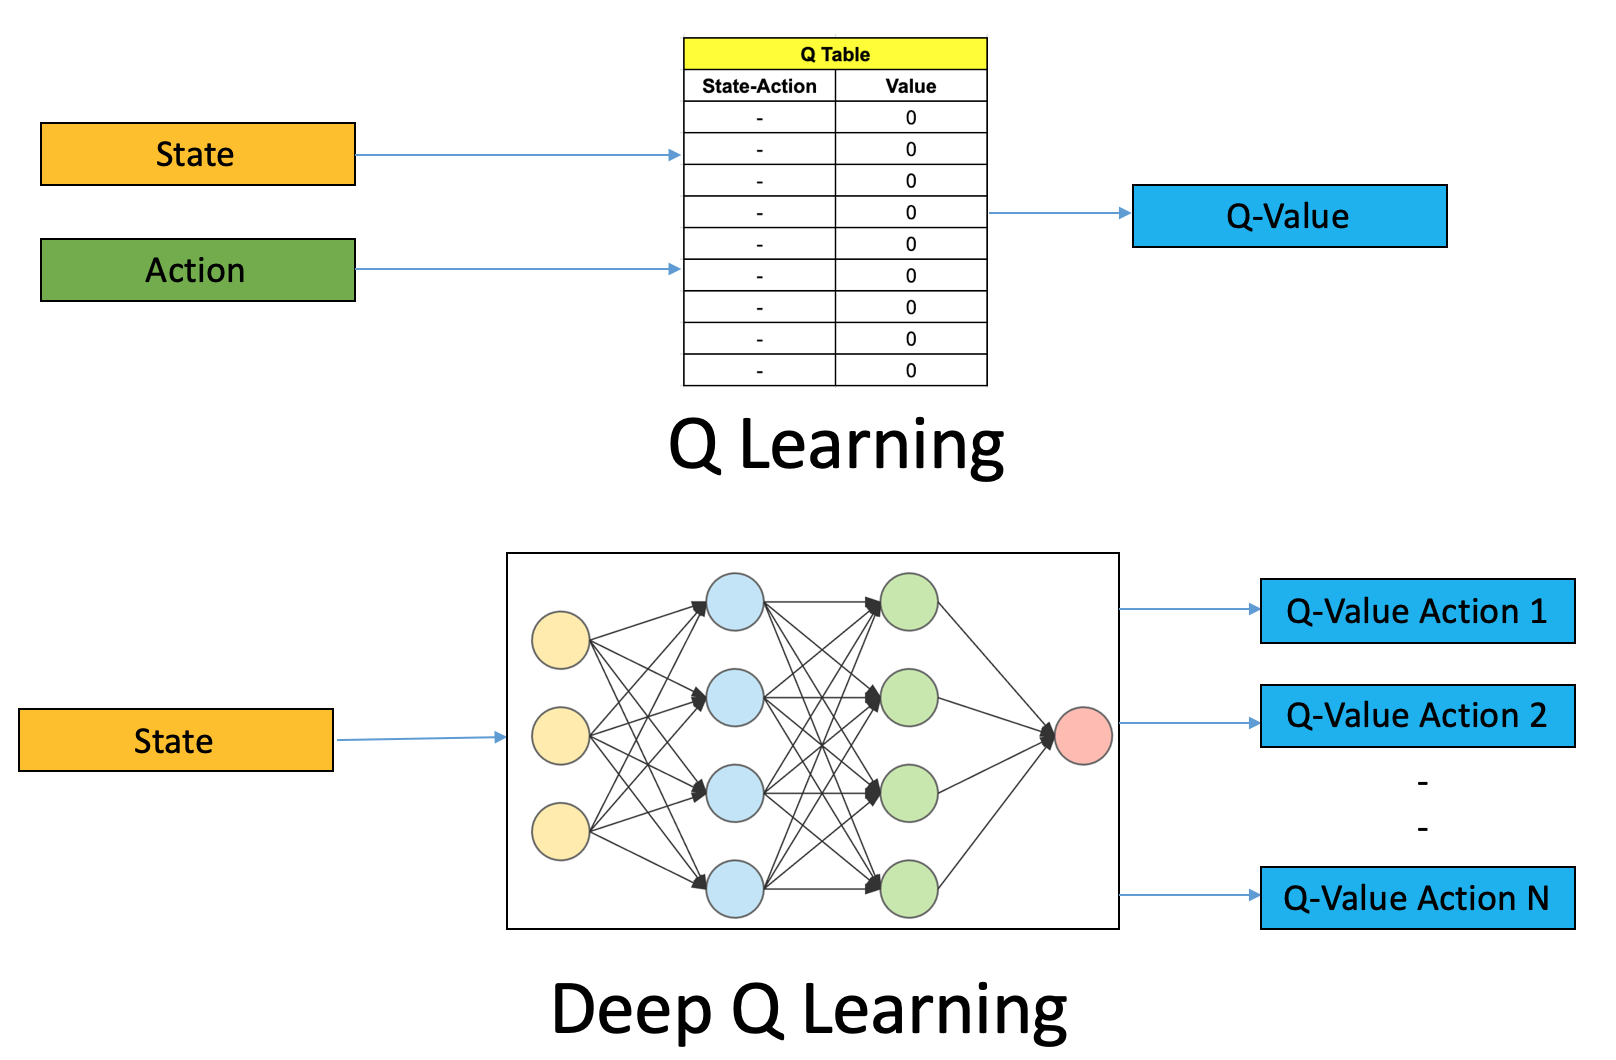
\includegraphics[scale=0.27]{chapter3/img/dqlearning.png}
        \end{center}
        \caption{Q-Learning và Deep Q-Learning}
        \label{fig:dqlearning}
    \end{figure}
\end{center}

Ta xét ví dụ sau, để làm rõ cách cập nhật trọng số của mạng nơ-ron và chọn ra hành động.

Giả sử, trạng thái hội thoại được rút gọn lại thành chỉ chứa các ý định hành động hiện tại của người dùng lần lượt là: hello, inform, request, reject, done. Ta mã hóa về dạng one-hot vec-tơ để làm đầu vào cho mạng nơ-ron. Các hành động có thể có của tác nhân là: hello, match\_found, request, done. Mạng nơ-ron huấn luyện trong ví dụ này như hình \ref{fig:examnetwork}. Activation của tầng ẩn là ReLU, tầng đầu ra là linear.

\begin{center}
    \begin{figure}[h!]
        \begin{center}
         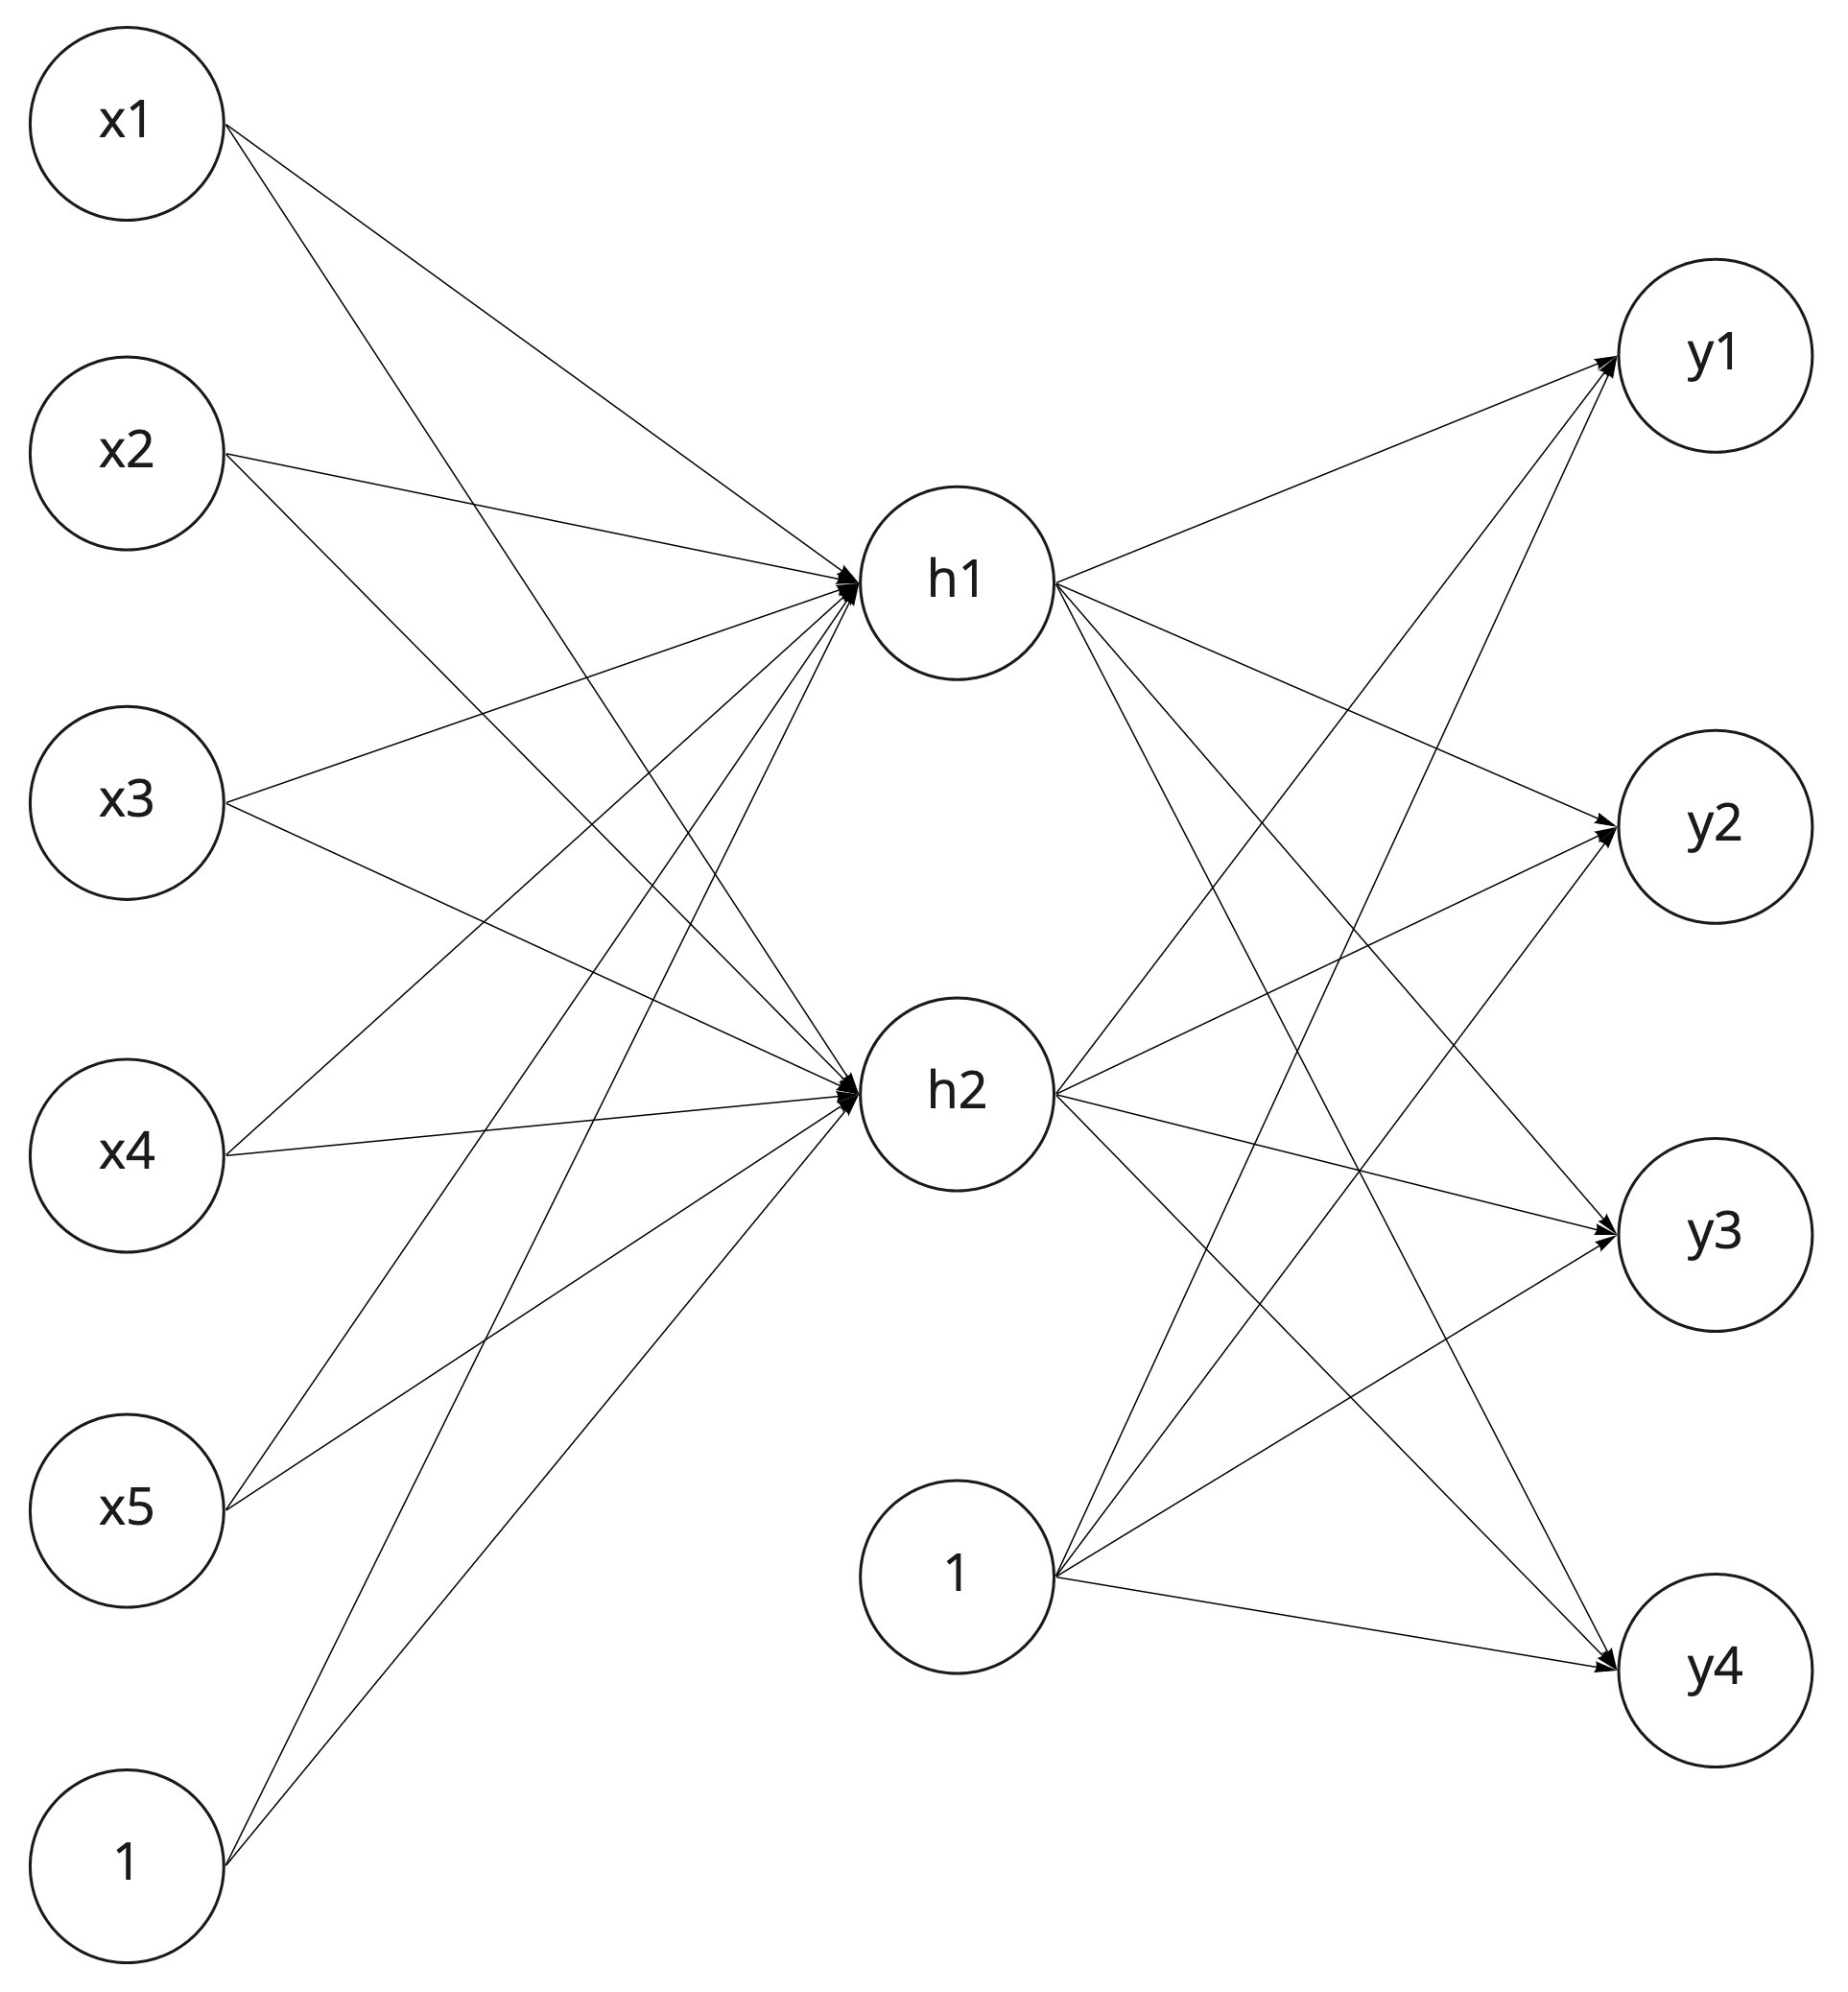
\includegraphics[scale=0.15]{chapter3/img/neural_network.jpg}
        \end{center}
        \caption{Mạng nơ-ron học sâu Q-Learing}
        \label{fig:examnetwork}
    \end{figure}
\end{center}

Giả sử, ta có ma trận trọng số cho mạng nơ-ron này như sau:

\begin{equation*}
    w_1 = 
    \begin{bmatrix}
        0.18998 & 0.871522 & 0.31542 & 0.691079 & 0.902874 \\
        0.12114 & 0.84606 & 0.902874 & 0.09224 & 0.19652302
    \end{bmatrix}
\end{equation*}

\begin{equation*}
    w_2 = 
    \begin{bmatrix}
        0.52141 & 0.63489 \\
        0.130012 & 0.12001 \\
        0.113114 & 0.12121 \\
        0.53514 & 0.62465
    \end{bmatrix}
\end{equation*}

\begin{equation*}
    bias = 0.325
\end{equation*}

\renewcommand{\lstlistingname}{Ví dụ}
\begin{lstlisting}[caption={Một mẫu đoạn hội thoại},label={exam:dialog3},language=exam_en,firstnumber=1]
User: hello
Agent: hello
User: request
Agent: match_found
User: done
\end{lstlisting}

Sử dụng đoạn hội thoại mẫu \ref{exam:dialog3} để huấn luyện. Ta có hành động đầu tiên của người dùng là hello. Trạng thái đầu vào $s$ như sau:

\begin{equation*}
    s = 
    \begin{bmatrix}
        1 \\
        0 \\
        0 \\
        0 \\
        0
    \end{bmatrix}
\end{equation*}

Sau khi cho qua mạng nơ-ron, ta có kết quả lần lượt là:

\begin{equation*}
    w_1*s + bias = 
    \begin{bmatrix}
        0.51498 \\
        0.44614
    \end{bmatrix}
\end{equation*}

\begin{equation*}
    h = relu(w_1*s + bias) = 
    \begin{bmatrix}
        0.51498 \\
        0.44614
    \end{bmatrix}
\end{equation*}

\begin{equation*}
    y = h*w_2 + bias = 
    \begin{bmatrix}
        0.876765546 \\
        0.445494841 \\
        0.437328077 \\
        0.879267748
    \end{bmatrix}
\end{equation*}

Kết quả ma trận y là giá trị Q cho từng hành động của tác nhân theo thứ tự là hello, match\_found, request, done. Với kết quả trên, ta thấy Q-value của hành động done là lớn nhất. Dễ thấy rằng, với hành động này, không hoàn thành được mục tiêu toàn cục. Vì vậy, ta cần cập nhật Q-value của hành động tốt nhất tại thời điểm này.

Vì done là hành vi kết thúc hội thoại, mà hiện tại nó chưa hoàn thành mục tiêu người dùng, nên nhận điểm trừ rất lớn là $r_0 = -10$. Nhìn lại công thức tính $Q^*$ mục tiêu. Giả sử $\gamma = 0.9$

\begin{equation*}
    Q^*(s,a) = r_0 + {\gamma}max_{a}Q^{*}(s',a)
\end{equation*}

Để có $Q(s',a)$, ta cho đầu vào mạng nơ-ron là trạng thái kế tiếp $s'$. Dựa vào mẫu hội thoại huấn luyện trên, ta có trạng thái đầu vào $s'$ như sau:

\begin{equation*}
    s' = 
    \begin{bmatrix}
        0 \\
        0 \\
        1 \\
        0 \\
        0
    \end{bmatrix}
\end{equation*}

Sau khi cho qua mạng nơ-ron, ta nhận được kết quả đầu ra là:

\begin{equation*}
    y = 
    \begin{bmatrix}
        1.438486316 \\
        0.555619444 \\
        0.546271075 \\
        1.434705853
    \end{bmatrix}
\end{equation*}

Ta có $Q$ lớn nhất với trạng thái đầu vào $s'$ là 1.438486316.

\begin{equation*}
    => Q^*(s,a) = -10 + 0.9*1.438486316 = -8.705362316
\end{equation*}

Sau đó, mô hình sẽ được huấn luyện lại với đầu vào là trạng thái $s$ và giá trị $Q$ được cập nhật lại như sau:

\begin{equation*}
    y = 
    \begin{bmatrix}
        0.876765546 \\
        0.445494841 \\
        0.437328077 \\
        -8.705362316
    \end{bmatrix}
\end{equation*}

\chapter{Phương pháp nghiên cứu}

\section{Kiến trúc tổng quát của hệ thống}
Để giải quyết các vấn đề đã được trình bày ở mục \ref{sec:muctieu}, hệ thống ứng dụng Chatbot tư vấn cần có ba module chính đó là phần UI/UX giao tiếp với người dùng, phần nhập dữ liệu và phần lõi của hệ thống.

\begin{center}
    \begin{figure}[h!]
        \begin{center}
         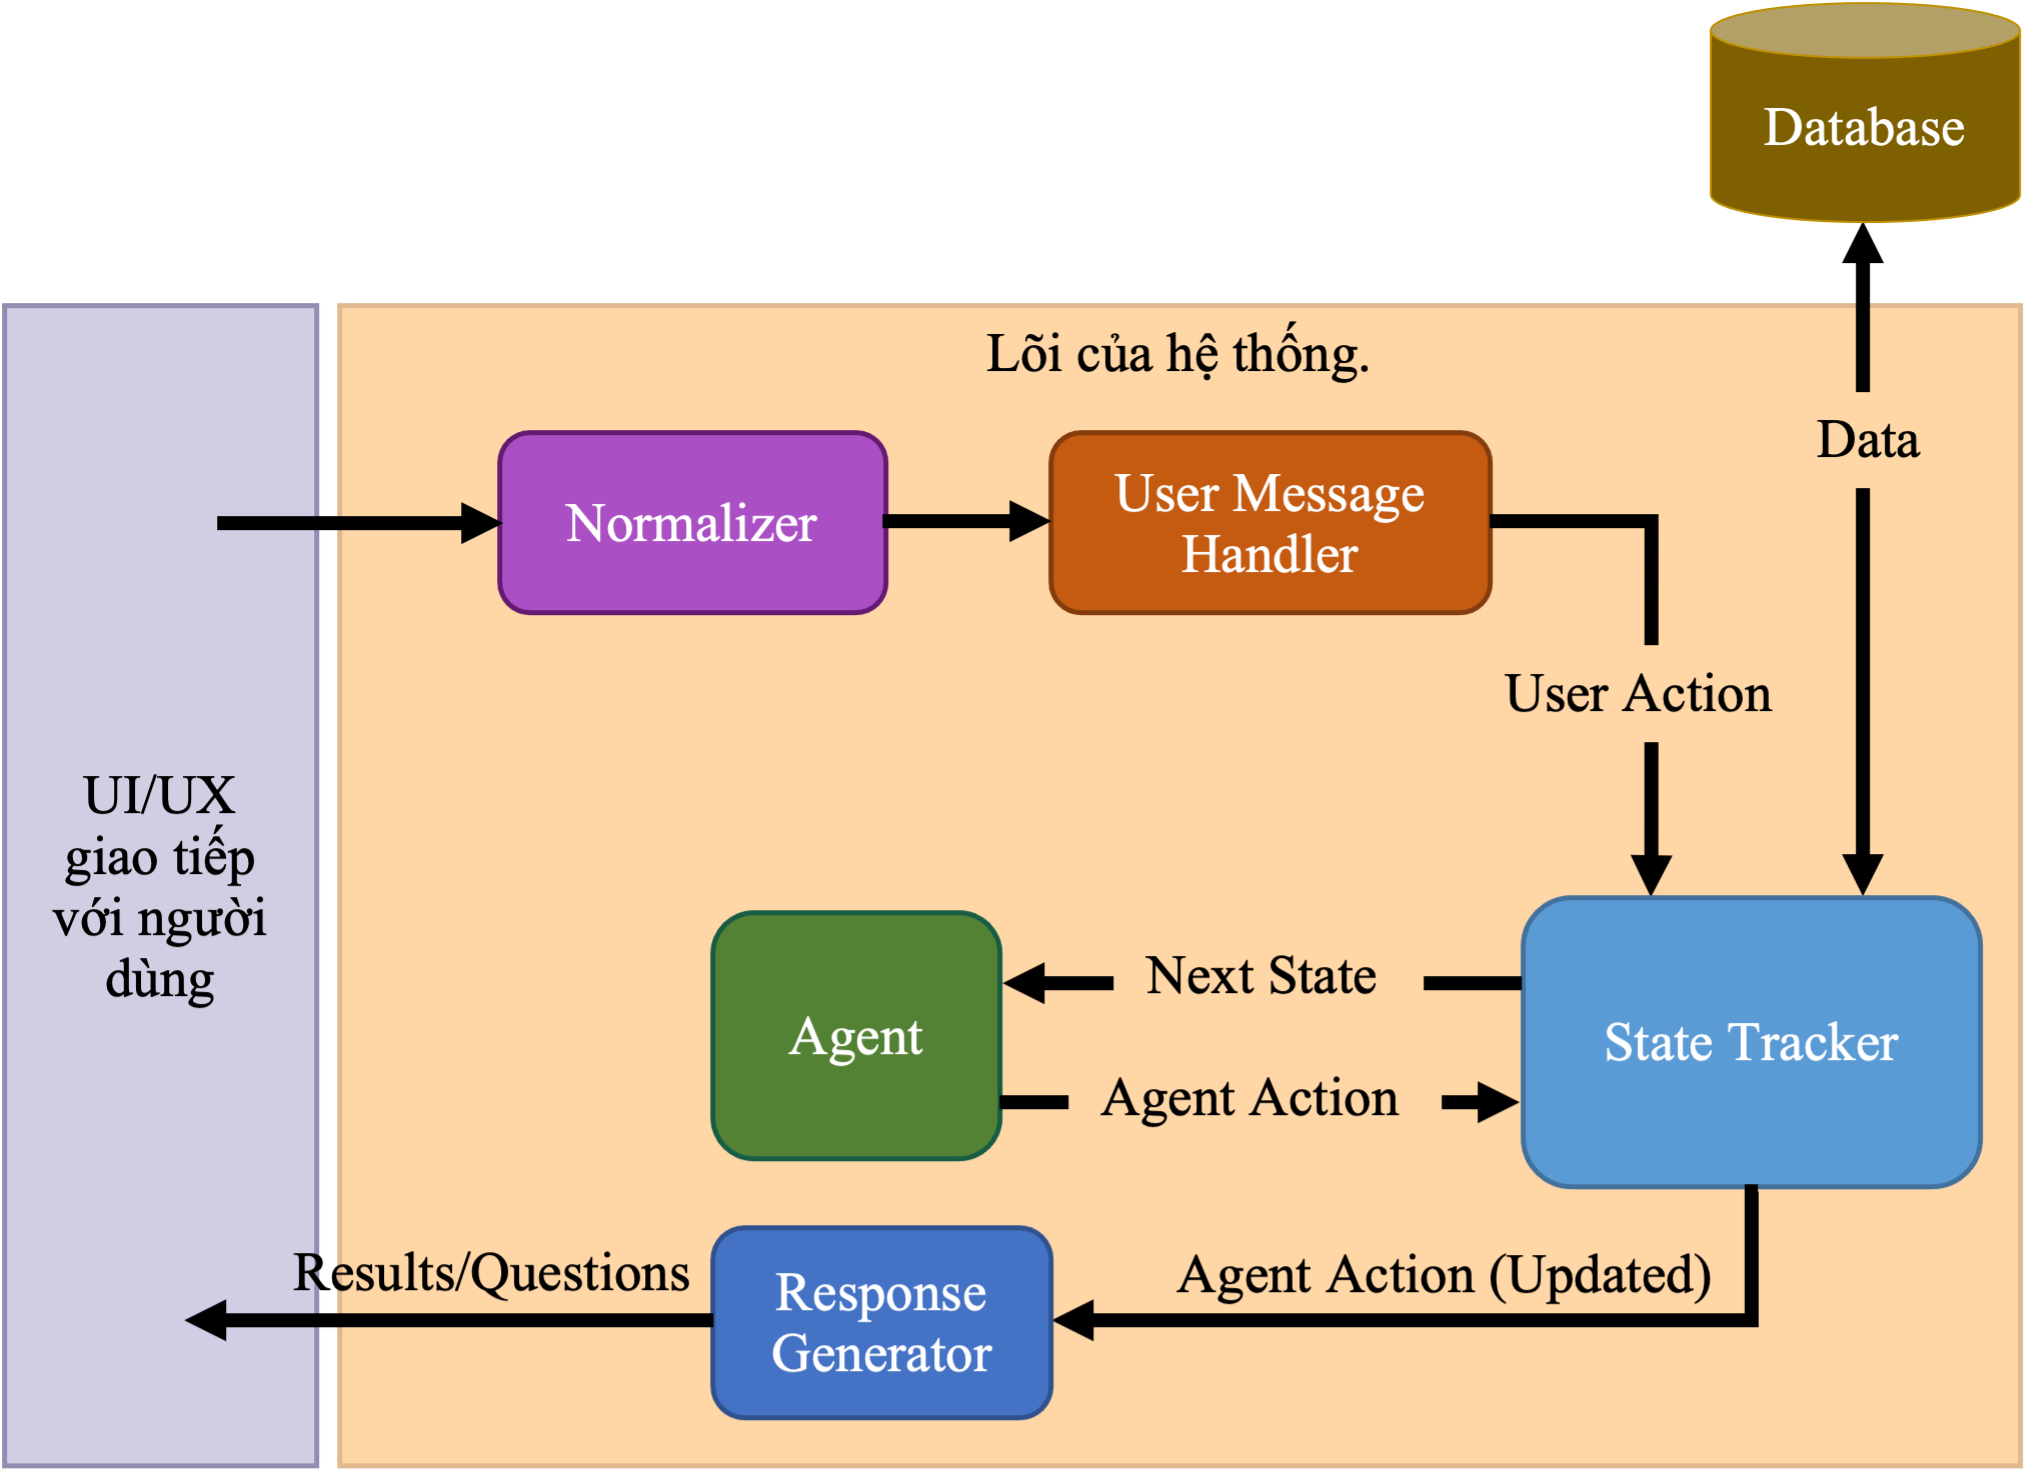
\includegraphics[scale=1]{chapter4/img/chatbot_app.png}
        \end{center}
        \caption{Kiến trúc tổng quát của ứng dụng Chatbot}
        \label{fig:chatbotapp}
    \end{figure}
\end{center}

Trong phần lõi của hệ thống, ta có các phần con khác như mô tả trong hình \ref{fig:chatbot}. Vì phạm vi của đề tài quá lớn nên trong đề tài này, chỉ thực hiện phần huấn luyện cho agent sử dụng phương pháp học tăng cường với mô hình Deep Q-Learning như được mô tả ở mục \ref{sec:model}, đồng thời xây dựng bộ mô phỏng người dùng và tạo lỗi để làm dữ liệu đầu vào cho việc huấn luyện mô hình. Các thành phần còn lại sẽ được tích hợp vào một hệ thống Chatbot có sẵn khác.

\section{Kiến trúc tổng quát của mô hình}
Đề tài áp dụng kiến trúc trong bài hướng dẫn \cite{traininggochatbot} được mô tả như hình \ref{fig:agentmodel}, cũng như sẽ có một số điều chỉnh để phù hợp với dữ liệu và yêu cầu của hệ thống sao cho đáp ứng được lĩnh vực đang thực hiện.

\begin{center}
    \begin{figure}[ht!]
        \begin{center}
         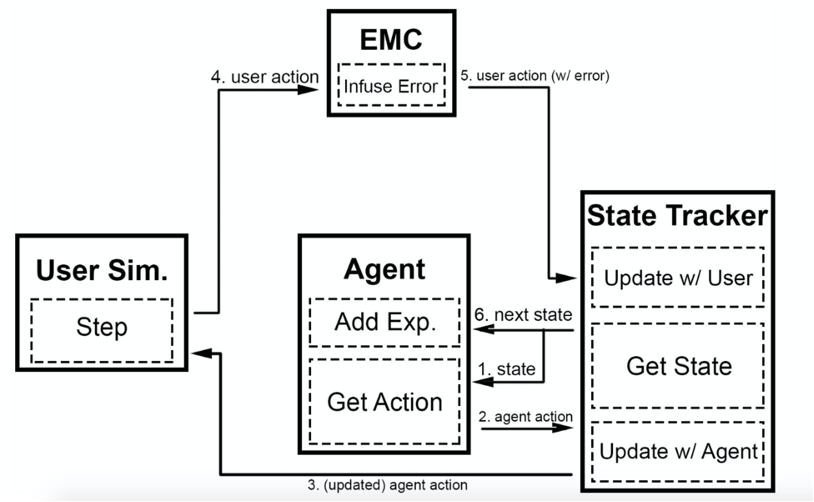
\includegraphics[scale=1]{chapter4/img/agentmodel.png}
        \end{center}
        \caption{Kiến trúc tổng quát của mô hình RL agent}
        \label{fig:agentmodel}
    \end{figure}
\end{center}

Kiến trúc này mô tả một vòng huấn luyện sẽ được diễn ra. Cụ thể:

\begin{itemize}
    \item \textbf{Bước 1:} Lấy ra \textit{state} - trạng thái hiện tại từ \textit{dialog state tracker}, \textit{state} này có thể là \textit{state} khởi tạo nếu như vừa bắt đầu hội thoại hoặc là \textit{state} của toàn bộ cuộc hội thoại giữa user và Chatbot. \textit{State} sau khi được lấy ra sẽ làm input (đầu vào) cho \textit{agent} ở bước tiếp theo.
    \item \textbf{Bước 2:} \textit{Agent} sau khi nhận được input từ bước trước sẽ sinh ra \textit{action} (hành động) và gửi ngược về lại \textit{dialog state tracker}. \textit{Action} lúc này ở dạng thô, chưa kèm thông tin cụ thể. Nó sẽ được \textit{dialog state tracker} cập nhật thông tin sau khi thực hiện truy vấn lên cơ sở dữ liệu. Đồng thời \textit{dialog state tracker} cũng sẽ cập nhật lại trạng thái của hội thoại.
    \item \textbf{Bước 3:} \textit{Action} sau khi được cập nhật đầy đủ thông tin sẽ được gửi cho \textit{user simulator}. \textit{User simulator} sẽ dựa vào các luật đã được quy định trước để sinh ra \textit{action} (có cấu trúc tương tự \textit{action} của \textit{agent} ở bước trước), kèm theo \textit{reward} (điểm thưởng) và tín hiệu success (thành công) để giúp \textit{agent} có thể tự điều chỉnh hành vi để học.
    \item \textbf{Bước 4:} \textit{Action} của user ở bước trước đó sẽ được đưa qua \textit{EMC}, mục đích là tạo ra các lỗi mà user thật hay mắc phải, giúp \textit{agent} có hành vi chính xác và tự nhiên hơn khi chạy ở thực tế.
    \item \textbf{Bước 5:} \textit{Action} ở bước trước sẽ tiếp tục được gửi đi đến \textit{dialog state tracker} và được cập nhật thông tin cụ thể tương tự ở bước 2. Đồng thời \textit{dialog state tracker} cũng cập nhật trạng thái của nó.
    \item \textbf{Bước 6:} Trạng thái tiếp theo được lấy từ \textit{dialog state tracker} và quay lại giống bước 1.
\end{itemize}

\section{Bộ mô phỏng người dùng (User Simulator)}
Mục đích của \textit{User Simulator} là dùng để mô phỏng người dùng thật để tương tác với \textit{agent} cũng như chấm điểm nó. Việc này sẽ tốn rất nhiều thời gian nếu như làm với người thật. Bộ \textit{User Simulator} này sẽ được hiện thực theo dạng luật định sẵn. Cụ thể với mỗi lần tham gia cuộc hội thoại (gọi là \textit{episode}), ta đều quy định sẵn các mục tiêu (\textit{user goal}) và thực hiện các \textit{action} phù hợp với mục tiêu đó, mỗi \textit{action} sẽ kèm theo các thông tin như \textit{slot} mà nó sẽ \textit{request} hay \textit{inform}.

\textit{User goal} có thể có được từ các cuộc hội thoại thực hoặc được làm thủ công (hoặc cả hai). Mỗi \textit{user goal} gồm các \textit{inform slots} và \textit{request slots}. Ví dụ, ta có một cuộc hội thoại sau đây:

\begin{verbatim}
Customer: [Hình ảnh sản phẩm] (mã sp là AT001)
Customer: Áo này có size XL không bạn?
Admin: Có bạn nha. 
Customer: Có những màu nào nữa vậy bạn.
Admin: Mẫu áo AT001 này có 3 màu ạ. Đỏ, Trắng, Đen.
\end{verbatim}

Trong cuộc hội thoại, khách hàng yêu cầu số lượng và màu sắc của sản phẩm với mã sản phẩm và kích thước mà họ cung cấp. Từ đó, ta sẽ có một \textit{user goal} như sau:

\begin{center}
\begin{lstlisting}[language=Java,breaklines=true]
{
    "request_slots": {
    	"amount": ["UNK"],
    	"color": ["UNK"]
    },
    "inform_slots": {
    	"name": ["AT001"],
    	"size": ["XL"]
    }
}
\end{lstlisting}
\end{center}

Khi quá trình huấn luyện diễn ra, tại mỗi \textit{episode}, bộ \textit{User Simulator} sẽ ngẫu nhiên chọn ra một \textit{user goal} từ một danh sách và sẽ lần lượt gửi các \textit{action} tương ứng phù hợp với \textit{user goal} đã được chọn tới \textit{agent}.

Để làm được điều trên, bộ \textit{User Simulator} cần phải lưu trữ trạng thái hội thoại cho riêng nó (trạng thái này khác với trạng thái của bộ \textit{dialog state tracker}). Trong đề tài này, nó sẽ được hiện thực theo cấu trúc dữ liệu dictionary trong Python, cụ thể:

\begin{itemize}
    \item \textbf{Rest slots:} Tất cả các \textit{inform slots} và \textit{request slots} từ \textit{user goal} mà \textit{agent} hoặc người dùng chưa được \textit{inform}.
    \item \textbf{History slots:} Tất cả các \textit{inform slots} từ các \textit{action} của người dùng và \textit{agent} cho đến thời điểm hiện tại.
    \item \textbf{Request slots:} Các \textit{request slots} mà người dùng muốn yêu cầu
    \item \textbf{Inform slots:} Các \textit{inform slots} sẽ được \textit{inform} cho \textit{agent} tại \textit{action} hiện tại.
    \item \textbf{Intent:} \textit{intent} của \textit{action} hiện tại.
\end{itemize}

Với mỗi \textit{action} nhận được từ \textit{agent}, tùy vào \textit{intent} mà \textit{User Simulator} sẽ phản hồi lại theo luật đã quy định sẵn:

Đầu tiên, kiểm tra số câu thoại đã thực hiện. Nếu số lần đến tối đa (20 lần) thì trả lời với "intent" = "done".

Nếu không thì tạo ra một \textit{action} dựa trên \textit{intent} của \textit{agent}:

\begin{itemize}
    \item "request": tuỳ thuộc vào \textit{request slots}, phản hồi với "intent" = "inform" hoặc "request".
    \item "inform": tuỳ thuộc vào trạng thái hiện tại của cuộc hội thoại, phản hồi với "intent" = "inform" hoặc "request" hoặc "thanks"
    \item "match\_found": tuỳ thuộc vào kết quả trả về của \textit{agent}, phản hồi với "intent" = "thanks" hoặc "reject"
    \item "done": phản hồi với "intent" = "done", đồng thời tuỳ thuộc vào trạng thái hội thoại mà quyết định cuộc hội thoại có thành công hay không.
\end{itemize}

Một trong những thành phần quan trọng trong giải thuật nêu trên là \textit{reward} - phần thưởng cho mỗi \textit{action} của \textit{agent}. Mỗi \textit{action} phản hồi của \textit{User Simulator} đều kèm theo điểm \textit{reward}. \textit{Reward} góp phần định hướng cho mỗi \textit{action} của \textit{agent}: khuyến khích bằng cách cho điểm cao trước mỗi \textit{action} chính xác hoặc dẫn đến thành công cho cuộc hội thoại, hoặc trừ điểm trước mỗi \textit{action} không phù hợp hoặc sai lầm để \textit{agent} có thể tránh lặp lại trong tương lai. \textit{Agent} sẽ tự điều chỉnh hành vi sao cho tổng điểm thưởng nhận được là lớn nhất khi kết thúc hội thoại. Một số điểm thưởng đã được định nghĩa như sau:

\begin{itemize}
    \item \textbf{NO OUTCOME:} chưa thể kết thúc cuộc hội thoại. Đây là giá trị mặc định mà trải qua mỗi lượt trong cuộc hội thoại \textit{agent} sẽ bị trừ và điểm trừ này là thấp nhất. Nó có tác dụng kích thích \textit{agent} mau chóng tìm ra kết quả để kết thúc hội thoại sớm nhất có thể.
    \item \textbf{UNSUITABLE:} phản hồi không phù hợp. Đây là điểm trừ khi \textit{agent} yêu cầu \textit{slot} mà người dùng đã yêu cầu từ trước, hoặc khi \textit{agent} yêu cầu lại \textit{slot} đã yêu cầu trước đó.
    \item \textbf{FAIL:} kết thúc hội thoại nhưng thất bại vì không thoả mãn người dùng. Đây là điểm trừ lớn nhất.
    \item \textbf{GOOD INFORM:} agent cung cấp giá trị hợp lý cho người dùng sẽ được cộng điểm thưởng khuyến khích hành vi này.
    \item \textbf{SUCCESS:} agent phản hồi kết quả thoả mãn yêu cầu của người dùng khi kết thúc cuộc hội thoại. Điểm cộng này là lớn nhất.
\end{itemize}

\section{Bộ giả lập lỗi (Error Model Controller)}
Sau khi nhận được \textit{action} tạo ra từ \textit{User Simulator}, nó sẽ được gửi đến bộ giả lập lỗi (EMC) để tạo ra các lỗi ngẫu nhiên. Việc này giúp \textit{agent} có thể xử lý được tốt hơn với các tình huống thực tế có thể phát sinh lỗi xuất phát từ các thành phần xử lý ngôn ngữ tự nhiên hoặc do người dùng mắc lỗi trong câu trả lời của họ. Các lỗi mà bộ phận này có thể tạo ra bao gồm lỗi ở \textit{slot} của \textit{inform} và \textit{intent} của \textit{action}. Cụ thể ở mức \textit{slot} ta có ba lỗi với xác suất xuất hiện bằng nhau:

\begin{itemize}
    \item Thay thế giá trị bằng một giá trị ngẫu nhiên cho \textit{slot} đó.
    \item Thay thế toàn bộ \textit{slot}: chọn \textit{slot} ngẫu nhiên và giá trị ngẫu nhiên cho \textit{slot} đó.
    \item Xóa \textit{slot}.
\end{itemize}

Đối với lỗi ở \textit{intent}, ta có thể tạo ra lỗi bằng cách thay thế \textit{intent} bằng một \textit{intent} ngẫu nhiên khác.

% \chapter {Kế hoạch triển khai}
Với những mục tiêu đã đề ra ở mục \ref{sec:muctieu}, đề tài được thực hiện qua các giai đoạn như sau:

\begin{itemize}
    \item \textbf{Giai đoạn 1:} Tìm kiếm và thu thập các thông tin về sản phẩm thời trang để thiết kế ra các hoạt động mà Chatbot có thể hỗ trợ.
    \item \textbf{Giai đoạn 2:} Khảo sát và thu thập các thông tin từ người dùng để thiết kế ra các ý định của người dùng.
    \item \textbf{Giai đoạn 3:} Định nghĩa cách kiểm thử và đánh giá hệ thống.
    \item \textbf{Giai đoạn 4:} Xây dựng bộ mô phỏng người dùng và lỗi.
    \item \textbf{Giai đoạn 5:} Xây dựng bộ quản lý hội thoại.
    \item \textbf{Giai đoạn 6:} Tích hợp các thành phần còn lại.
    \item \textbf{Giai đoạn 7:} Tiến hành kiểm thử và đánh giá hệ thống.
\end{itemize}

Thời gian cụ thể thực hiện được mô tả như sau:

\begin{center}
    \begin{figure}[h!]
        \begin{center}
         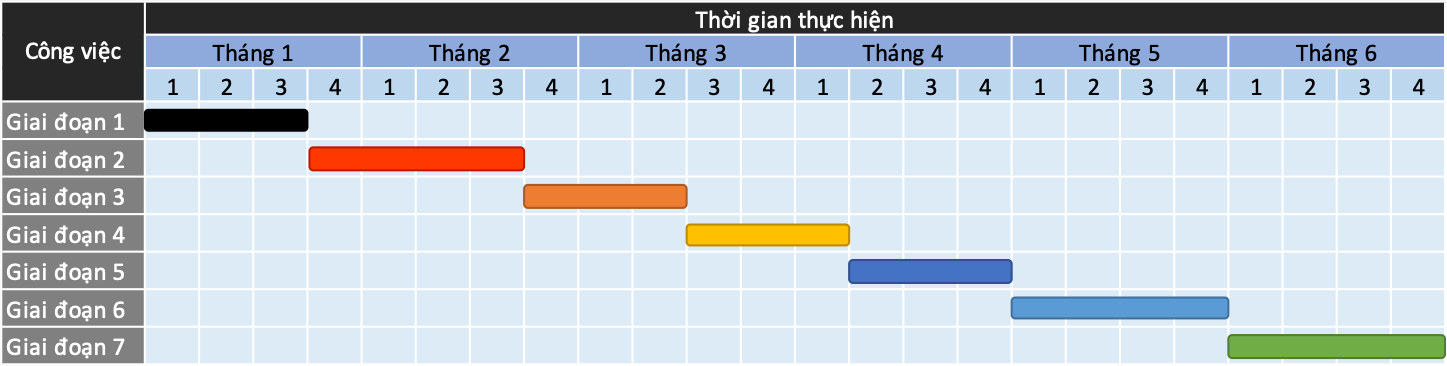
\includegraphics[scale=0.63]{chapter4.5/img/timeline.png}
        \end{center}
        \caption{Thời gian thực hiện đề tài}
    \end{figure}
\end{center}
\chapter{Công nghệ sử dụng}

\section{Ngôn ngữ lập trình}
\subsection{Python}
Python là một ngôn ngữ lập trình bậc cao cho các mục đích lập trình đa năng, do Guido van Rossum tạo ra và lần đầu ra mắt vào năm 1991 và được phát triển trong một dự án mã nguồn mở. Python sử dụng cơ chế cấp phát bộ nhớ động, hỗ trợ các phương thức lập trình như lập trình hướng đối tượng, lập trình hàm.

Python được thiết kế với ưu điểm mạnh là dễ đọc, dễ học và dễ nhớ. Python là ngôn ngữ có hình thức rất sáng sủa, cấu trúc rõ ràng, thuận tiện cho người mới học lập trình và là ngôn ngữ lập trình dễ học, được dùng rộng rãi trong phát triển trí tuệ nhân tạo.

Python hỗ trợ rất mạnh về Machine Learning, Deep Learning với các thư viện như TensorFlow, Pytorch, Keras, ... Ngoài ra còn có các thư viện hỗ trợ mạnh cho việc xử lý dữ liệu như là Pandas, Numpy, Scipy, ...

Trong đề tài này sử dụng phiên bản Python 3.8 để hiện thực các thành phần trong hệ thống.

\subsection{JavaSrcipt}
JavaScript được tạo trong mười ngày bởi Brandan Eich, một nhân viên của Netscape, vào tháng 9 năm 1995. JavaScript liên tục phát triển kể từ đó. Chỉ sau 20 năm, nó từ một ngôn ngữ lập trình riêng trở thành công cụ quan trọng nhất trên bộ công cụ của các chuyên viên lập trình web.

Một số đặc điểm của JavaScript:

\begin{itemize}
    \item Là một ngôn ngữ lập trình thông dịch.
    \item Không cần một compiler vì web browser có thể biên dịch nó bằng HTML.
    \item Dễ học và dễ sử dụng hơn các ngôn ngữ lập trình khác.
    \item Hoạt động trên nhiều trình duyệt, nền tảng.
\end{itemize}

JavaScript được dùng rộng rãi cho các trang web (phía người dùng) cũng như phía máy chủ, cũng là một lý do khiến nó trở nên rất phổ biến.

\subsection{HTML}
HTML được tạo ra bởi Tim Berners-Lee, một nhà vật lý học của trung tâm nghiên cứu CERN ở Thụy Sĩ. Hiện nay, HTML đã trở thành một chuẩn Internet được tổ chức W3C (World Wide Web Consortium) vận hành và phát triển.

HTML viết tắt của Hypertext Markup Language, tạm dịch là ngôn ngữ đánh dấu siêu văn bản, là ngôn ngữ lập trình dùng để xây dựng và cấu trúc lại các thành phần có trong Website. Nó có thể được trợ giúp bởi các công nghệ như CSS và các ngôn ngữ kịch bản giống như JavaScript.

Một số đặc điểm của HTML:

\begin{itemize}
    \item Đây là một ngôn ngữ đơn giản rất dễ học và dễ sử dụng.
    \item Rất dễ dàng để trình bày hiệu quả với HTML vì nó có nhiều thẻ định dạng.
    \item Đây là một ngôn ngữ đánh dấu vì vậy có thể sử dụng nó một cách linh hoạt để thiết kế trang web cùng với văn bản.
    \item Hoạt động trên nhiều trình duyệt, nền tảng.
\end{itemize}

\subsection{CSS}
CSS là chữ viết tắt của Cascading Style Sheets, nó là một ngôn ngữ được sử dụng để tìm và định dạng lại các phần tử được tạo ra bởi các ngôn ngữ đánh dấu (HTML). Nói ngắn gọn hơn là ngôn ngữ tạo phong cách cho trang web. Nếu HTML đóng vai trò định dạng các phần tử trên website như việc tạo ra các đoạn văn bản, các tiêu đề, bảng, ... thì CSS sẽ giúp chúng ta có thể thêm style vào các phần tử HTML đó như đổi bố cục, màu sắc trang, đổi màu chữ, font chữ, thay đổi cấu trúc, ...

CSS được phát triển bởi W3C (World Wide Web Consortium) vào năm 1996, vì HTML không được thiết kế để gắn tag để giúp định dạng trang web.

Mối tương quan giữa HTML và CSS rất mật thiết. HTML là ngôn ngữ markup (nền tảng của site) và CSS định hình phong cách (tất cả những gì tạo nên giao diện website), chúng là không thể tách rời.

\subsection{JSON}
JSON là chữ viết tắt của Javascript Object Notation, đây là một dạng dữ liệu tuân theo một quy luật nhất định mà hầu hết các ngôn ngữ lập trình hiện nay đều có thể đọc được. 

Định dạng JSON giống cú pháp mã tạo đối tượng Javascript. JSON sử dụng cú pháp Javascript, nhưng định dạng JSON chỉ văn bản như XML. Ta có thể sử dụng lưu nó vào một tệp (file), một bản ghi (record) trong cơ sở dữ liệu rất dễ dàng. 

JSON có định dạng đơn giản, là một dạng trao đổi dữ liệu trọng lượng nhẹ (lightweight data-interchange format), xử lý nhanh, dễ hiểu, dễ dàng sử dụng hơn XML rất nhiều nên tính ứng dụng của nó hiện nay rất là phổ biến, trong tương lai tới, các ứng dụng sẽ sử dụng JSON là đa số.

\section{Nền tảng và thư viện}
\subsection{Pandas}
Pandas là một thư viện phần mềm được viết cho ngôn ngữ lập trình Python để thao tác và phân tích dữ liệu. Với Pandas, người dùng có thể dễ dàng tạo ra các bảng dữ liệu (Dataframe) và thực hiện các phép truy vấn, thống kê trên nó, cho phép đọc/ghi các định dạng file một cách dễ dàng.

\subsection{TensorFlow}
TensorFlow là một thư viện phần mềm mã nguồn mở dành cho máy học trong nhiều loại hình tác vụ nhận thức và hiểu ngôn ngữ.

TensorFlow nguyên thủy được phát triển bởi đội Google Brain cho mục đích nghiên cứu và sản xuất của Google và sau đó được phát hành theo giấy phép mã nguồn mở Apache 2.0.

TensorFlow tích hợp sẵn rất nhiều các thư viện Machine Learning, Deep Learning, có khả năng tương thích và mở rộng tốt. Trong đề tài này, sử dụng nó trong việc xây dựng mạng Deep Q-Learning.

\subsection{Keras}
Keras là một thư viện mạng nơ ron được viết bằng Python năm 2015 bởi một kỹ sư Deep Learning của Google. Ta có thể kết hợp Keras với các thư viện Deep Learning. Keras được phát triển với trọng tâm là cho phép thử nghiệm nhanh, việc thử nghiệm nhanh đôi khi sẽ mang lại kết quả nghiên cứu tốt. Trong đề tài này, sử dụng Keras trong việc xây dựng mô hình Deep Q-Learning.

\subsection{Eel}
Eel là một thư viện Python nhỏ để tạo các ứng dụng GUI ngoại tuyến HTML/JS đơn giản, với toàn quyền truy cập vào các khả năng và thư viện Python. Eel lưu trữ một máy chủ web cục bộ, sau đó cho phép chú thích các hàm bằng Python để chúng có thể được gọi từ Javascript và ngược lại. Eel được thiết kế để giảm bớt rắc rối khi viết các ứng dụng GUI ngắn và đơn giản.

\section{Công cụ}
\subsection{Google Colab}
Colaboratory hay còn gọi là Google Colab, là một sản phẩm từ Google Research, nó cho phép chạy các dòng code python thông qua trình duyệt, đặc biệt phù hợp với Data analysis, machine learning và giáo dục. Colab không cần yêu cầu cài đặt hay cấu hình máy tính, mọi thứ có thể chạy thông qua trình duyệt, có thể sử dụng tài nguyên máy tính từ CPU tốc độ cao và cả GPUs và cả TPUs đều được cung cấp.

\chapter{Hiện thực hệ thống}

\section{Dữ liệu}
\label{sec:database}
Dưới sự hỗ trợ của một cửa hàng thời trang thực tế (Thời trang Hume), đề tài thực hiện việc chuẩn hóa và gán nhãn cho các dữ liệu về sản phẩm, phục vụ cho nhu cầu tư vấn của người dùng. Ngoài ra, đề tài còn thu thập và tổng hợp một số loại dữ liệu khác phục vụ cho các mục đích khác nhau.

\subsection{Dữ liệu sản phẩm}
\label{subsec:productdb}
Dữ liệu sản phẩm này chứa các thông tin sản phẩm dùng để tư vấn, tìm kiếm cho khách hàng một sản phẩm phù hợp với yêu cầu, một bản ghi trong cơ sở dữ liệu tương ứng với một sản phẩm. Mỗi trường thông tin của sản phẩm có thể có các định dạng khác nhau. Cụ thể:

\begin{itemize}
    \item \textbf{name\_product:} tên của sản phẩm, có thể có nhiều alias của tên sản phẩm trong cơ sở dữ liệu sản phẩm, thuộc kiểu dữ liệu chuỗi ký tự (string).
    \item \textbf{size\_product:} kích cỡ của sản phẩm, có thể có nhiều alias của kích cỡ sản phẩm trong cơ sở dữ liệu sản phẩm, thuộc kiểu dữ liệu chuỗi ký tự (string).
    \item \textbf{color\_product:} màu sắc của sản phẩm, có thể có nhiều alias của màu sắc sản phẩm trong cơ sở dữ liệu sản phẩm, thuộc kiểu dữ liệu chuỗi ký tự (string).
    \item \textbf{material\_product:} chất liệu của sản phẩm, có thể có nhiều alias của chất liệu sản phẩm trong cơ sở dữ liệu sản phẩm, thuộc kiểu dữ liệu chuỗi ký tự (string).
    \item \textbf{cost\_product:} đơn giá của sản phẩm, có thể có nhiều alias của đơn giá sản phẩm trong cơ sở dữ liệu sản phẩm, thuộc kiểu dữ liệu chuỗi ký tự (string).
    \item \textbf{amount\_product:} số lượng sản phẩm hiện tại, có thể có nhiều alias của số lượng sản phẩm trong cơ sở dữ liệu sản phẩm, thuộc kiểu dữ liệu số (int).
\end{itemize}

Bản ghi mẫu của dữ liệu sản phẩm như ví dụ \ref{exam:productrecord}.

\renewcommand{\lstlistingname}{Ví dụ}
\begin{lstlisting}[caption={Một bản ghi của dữ liệu sản phẩm},label={exam:productrecord},language=code_vn,firstnumber=1]
{
    "name_product": "set trắng cổ nơ",
    "size_product": "M",
    "color_product": "None",
    "cost_product": "260",
    "material_product": "vải cao cấp, mặc mát",
    "amount_product": 10
}
\end{lstlisting}

\subsection{Dữ liệu kích cỡ}
\label{subsec:sizedb}
Dữ liệu kích cỡ này chứa các thông tin về kích thước dùng để tư vấn, tìm kiếm cho khách hàng một kích cỡ sản phẩm phù hợp với số đo cơ thể, một bản ghi trong cơ sở dữ liệu tương ứng với một bảng kích thước. Mỗi trường thông tin của dữ liệu có thể có các định dạng khác nhau. Các giá trị của cùng một thông tin có cùng một đơn vị. Cụ thể:

\begin{itemize}
    \item \textbf{size\_customer:} kích cỡ sản phẩm phù hợp với khách hàng, có thể có nhiều alias của kích cỡ sản phẩm trong cơ sở dữ liệu kích cỡ, thuộc kiểu dữ liệu chuỗi ký tự (string).
    \item \textbf{waist\_customer:} số đo vòng eo của cơ thể, có thể có nhiều alias của số đo vòng eo trong cơ sở dữ liệu kích cỡ, thuộc kiểu dữ liệu chuỗi ký tự (string), đơn vị là centimet (cm).
    \item \textbf{height\_customer:} số đo chiều cao của cơ thể, có thể có nhiều alias của số đo chiều cao trong cơ sở dữ liệu kích cỡ, thuộc kiểu dữ liệu chuỗi ký tự (string), đơn vị là centimet (cm).
    \item \textbf{weight\_customer:} số đo cân nặng của cơ thể, có thể có nhiều alias của số đo cân nặng trong cơ sở dữ liệu kích cỡ, thuộc kiểu dữ liệu chuỗi ký tự (string), đơn vị là kilogram (kg).
\end{itemize}

Bản ghi mẫu của dữ liệu kích cỡ như ví dụ \ref{exam:sizerecord}.

\renewcommand{\lstlistingname}{Ví dụ}
\begin{lstlisting}[caption={Một bản ghi của dữ liệu kích cỡ},label={exam:sizerecord},language=code_vn,firstnumber=1]
{
    "size_customer": "S",
    "waist_customer": "65",
    "height_customer": "164",
    "weight_customer": "50"
}
\end{lstlisting}

\subsection{Từ điển thông tin sản phẩm}
Từ điển (Dictionary) của thông tin sản phẩm chứa tất cả các giá trị có thể có của từng thông tin sản phẩm (như mô tả ở mục \ref{subsec:productdb}). Dữ liệu được sử dụng để tạo ra các \textit{User Goal} (mục tiêu người dùng), phục vụ cho việc huấn luyện. Ngoài ra được sử dụng bởi \textit{EMC} (bộ giả lập lỗi), bộ tạo ra các lỗi ngẫu nhiên của người dùng. Mỗi trường thông tin có định dạng danh sách (array). Được biểu diễn rút gọn như ví dụ \ref{exam:dictproduct}.

\renewcommand{\lstlistingname}{Ví dụ}
\begin{lstlisting}[caption={Từ điển thông tin sản phẩm},label={exam:dictproduct},language=code_vn,firstnumber=1]
{
    "name_product": ["đầm nude cổ vest dáng dài", "đầm sơ mi carô", "set hồng vest váy ngắn", "đầm nude lưới tay phồng", ...],
    "size_product": ["S", "M", "L", ...],
    "color_product": ["nude", "carô xanh", "hồng", "xanh", ...],
    "cost_product": ["280", "210", "260", "238", "195", "350", ...],
    "material_product": ["vải cao cấp, mặc mát", ...],
    "amount_product": ["2", "5", "hai", "9", "ba", "4", "3", "6", ...]
}
\end{lstlisting}

\subsection{Từ điển dữ liệu kích cỡ}
Từ điển (Dictionary) của bảng dữ liệu kích cỡ chứa tất cả các giá trị có thể có của từng trường thông tin trong dữ liệu kích cỡ (như mô tả ở mục \ref{subsec:sizedb}). Dữ liệu được sử dụng để tạo ra các \textit{User Goal} (mục tiêu người dùng), phục vụ cho việc huấn luyện. Ngoài ra được sử dụng bởi \textit{EMC} (bộ giả lập lỗi), bộ tạo ra các lỗi ngẫu nhiên của người dùng. Mỗi trường thông tin có định dạng danh sách (array). Được biểu diễn rút gọn như ví dụ \ref{exam:dictsize}.

\renewcommand{\lstlistingname}{Ví dụ}
\begin{lstlisting}[caption={Từ điển dữ liệu kích cỡ},label={exam:dictsize},language=code_vn,firstnumber=1]
{
    "size_customer": ["L", "S", "M"],
    "waist_customer": ["anything", "66", "73", "68", "63", "58", ...],
    "height_customer": ["163", "159", "166", "150", "anything", "155", "165", "156", ...],
    "weight_customer": ["56", "45", "47", "46", "57", "48", "41", "52", "anything", ...]
}
\end{lstlisting}

\subsection{Mục tiêu người dùng (User Goal)}
\label{subsec:usergoal}
Mục tiêu người dùng (User Goal) chứa danh sách các trường hợp biểu diễn mục tiêu có thể có của người dùng. Dữ liệu được sử dụng bởi bộ mô phỏng người dùng sử dụng như mục tiêu thật của người dùng, phục vụ cho quá trình huấn luyện. Mỗi \textit{goal} chỉ chứa cho một mục tiêu xuyên suốt cuộc hội thoại. Cấu trúc cho một \textit{goal} như sau:

\begin{itemize}
    \item \textbf{intent:} mục tiêu chính của người dùng trong cuộc hội thoại, kiểu dữ liệu chuỗi ký tự (string). Các mục tiêu khi tham gia hội thoại của người dùng có thể có là:
    \begin{itemize}
        \item \textbf{request:} yêu cầu thông tin sản phẩm, hoặc tư vấn kích cỡ sản phẩm cho khách hàng
        \item \textbf{order:} mục tiêu đặt hàng sản phẩm của khách hàng
    \end{itemize}
    \item \textbf{inform\_slots:} chứa tất cả các thông tin cần thông báo cho tác nhân trong suốt cuộc hội thoại. Các thông tin cần thông báo có cấu trúc <tên thông tin>: <giá trị của thông tin>. Trong đó:
    \begin{itemize}
        \item \textbf{<tên thông tin>:} tên thông tin là một trong các trường thông tin đã được định nghĩa ở mục \ref{subsec:productdb} và \ref{subsec:sizedb}.
        \item \textbf{<giá trị của thông tin>:} giá trị của thông tin này có thể nằm trong bộ từ điển của nó hoặc không.
    \end{itemize}
    \item \textbf{request\_slots:} chứa tất cả các thông tin yêu cầu tác nhân cung cấp cho đến khi kết thúc cuộc hội thoại. Các thông tin yêu cầu có cấu trúc <tên thông tin>: "UNK". Trong đó:
    \begin{itemize}
        \item \textbf{<tên thông tin>:} tên thông tin là một trong các trường thông tin đã được định nghĩa ở mục \ref{subsec:productdb} và \ref{subsec:sizedb}.
        \item \textbf{"UNK":} giá trị mặc định, có nghĩa "chưa biết", cần được thông báo/ điền vào từ tác nhân.
    \end{itemize}
\end{itemize}

Bản ghi mẫu của mục tiêu người dùng như ví dụ \ref{exam:goalrecord}.

\renewcommand{\lstlistingname}{Ví dụ}
\begin{lstlisting}[caption={Một bản ghi của mục tiêu người dùng},label={exam:goalrecord},language=code_vn,firstnumber=1]
{
    "intent": "request",
    "inform_slots": {
        "name_product": "set dây kèm quần",
        "amount_product": "4",
        "color_product": "đen viền",
        "waist_customer": "63",
        "height_customer": "158",
        "weight_customer": "59"
    },
    "request_slots": {
        "size_product": "UNK",
        "material_product": "UNK",
        "cost_product": "UNK"
    }
}
\end{lstlisting}

\subsection{Hội thoại (Dialog)}
Dữ liệu hội thoại (Dialog) chứa danh sách các cuộc hội thoại tư vấn, như mô tả ở mục \ref{subsubsec:dialog}. Dữ liệu được sử dụng cho giai đoạn khởi động. Mỗi \textit{dialog} mô tả quá trình hội thoại tư vấn diễn ra như trong thực tế, chứa danh sách các hành động lần lượt là của người dùng và tác nhân, mỗi hành động có cấu trúc như sau:

\begin{itemize}
    \item \textbf{speaker:} mô tả lượt hành động do người dùng hay tác nhân thực hiện, kiểu dữ liệu là chuỗi ký tự (string).
    \item \textbf{intent:} ý định hành động của người dùng hoặc tác nhân trong lượt thoại hiện tại, kiểu dữ liệu chuỗi ký tự (string). Các mục tiêu có thể có được mô tả ở bảng \ref{tab:userintent}.
    \item \textbf{inform\_slots:} chứa các thông tin cần thông báo trong lượt thoại hiện tại. Các thông tin cần thông báo có cấu trúc <tên thông tin>: <giá trị của thông tin>. Trong đó:
    \begin{itemize}
        \item \textbf{<tên thông tin>:} tên thông tin là một trong các trường thông tin đã được định nghĩa ở mục \ref{subsec:productdb} và \ref{subsec:sizedb}.
        \item \textbf{<giá trị của thông tin>:} giá trị của thông tin này có thể nằm trong bộ từ điển của nó hoặc không.
    \end{itemize}
    \item \textbf{request\_slots:} chứa các thông tin yêu cầu đối phương cung cấp trong lượt thoại hiện tại. Trường thông tin yêu cầu này là danh sách các thông tin có kiểu dữ liệu là chuỗi ký tự (string).
    \begin{itemize}
        \item \textbf{<tên thông tin>:} tên thông tin là một trong các trường thông tin đã được định nghĩa ở mục \ref{subsec:productdb} và \ref{subsec:sizedb}.
    \end{itemize}
\end{itemize}

Bản ghi mẫu của hội thoại như ví dụ \ref{exam:dialogrecord}.

\renewcommand{\lstlistingname}{Ví dụ}
\begin{lstlisting}[caption={Một đoạn hội thoại},label={exam:dialogrecord},language=code_vn,firstnumber=1]
[
    {"speaker": "user", "intent": "request", "inform_slots": {}, "request_slots": ["cost_product"]},
    {"speaker": "agent", "intent": "request", "inform_slots": {}, "request_slots": ["name_product"]},
    {"speaker": "user", "intent": "inform", "inform_slots": {"name_product": "đầm body vest"}, "request_slots": []},
    {"speaker": "agent", "intent": "inform", "inform_slots": {"cost_product": "260"}, "request_slots": []},
    {"speaker": "user", "intent": "ok", "inform_slots": {}, "request_slots": []},
    {"speaker": "agent", "intent": "match_found", "inform_slots": {}, "request_slots": []},
    {"speaker": "user", "intent": "ok", "inform_slots": {}, "request_slots": []},
    {"speaker": "agent", "intent": "done", "inform_slots": {}, "request_slots": []},
    {"speaker": "user", "intent": "done", "inform_slots": {}, "request_slots": []}
]
\end{lstlisting}

\section{Bộ xử lý phản hồi người dùng}
Do giới hạn của đề tài, trong luận án này không xử lý ngôn ngữ tự nhiên cho các câu phản hồi của người dùng. Tuy nhiên, hệ thống có thể tích hợp với bộ xử lý ngôn ngữ tự nhiên khác. Trong bộ xử lý phản hồi người dùng này, hệ thống sẽ tiến hành xử lý các thông tin nhập vào từ giao diện hệ thống Chabot hoặc kết quả trả về từ bộ xử lý ngôn ngữ tự nhiên bên ngoài thành một cấu trúc đồng nhất để sử dụng trong lõi hệ thống, lõi hệ thống như mô tả ở hình \ref{fig:chatbotapp}. Các hành động được biểu diễn như cấu trúc \ref{struct:action}.

\renewcommand{\lstlistingname}{Cấu trúc}
\begin{lstlisting}[caption={Cấu trúc cho một hành động},label={struct:action},language=structure,firstnumber=1]
{
    "intent": <value 1>,
    "inform_slots": <value 2>,
    "request_slots": <value 3>
}
\end{lstlisting}

Trong đó:

\begin{itemize}
    \item \textbf{<value 1>}: chứa ý định người dùng, các giá trị hợp lệ được mô tả trong bảng \ref{tab:userintent}
    \item \textbf{<value 2>}: là một dictionary (kiểu dữ liệu của Python), có cấu trúc key:value, với key là tên thông tin cung cấp, các trường thông tin được định nghĩa ở mục \ref{subsec:productdb} và \ref{subsec:sizedb}, value là giá trị của thông tin
    \item \textbf{<value 3>}: là một dictionary, có cấu trúc key:value, với key là tên thông tin yêu cầu, các trường thông tin được định nghĩa ở mục \ref{subsec:productdb} và \ref{subsec:sizedb}, value có giá trị mặc định là chuỗi kí tự "UNK".
\end{itemize}

\begin{table}[!ht]
\caption{Các ý định hành động của người dùng}
\centering
\begin{tabular}{|p{1cm}|c|p{11cm}|}
\hline
\centering\textbf{STT} & 
\centering\textbf{Ý định} & 
\parbox[t]{11cm}{\centering\textbf{Mô tả}} \\ % inserts table %heading
\hline
\centering 1 & 
hello & 
Ý định khi người dùng thực hiện các câu chào, hỏi thăm với tác nhân \\
\hline
\centering 2 & 
inform & 
Ý định khi người dùng cần thông báo thông tin đến cho tác nhân \\
\hline
\centering 3 & 
request & 
Ý định khi người dùng yêu cầu tác nhân cung cấp thông tin \\
\hline
\centering 4 & 
order & 
Ý định khi người dùng muốn đặt hàng sản phẩm \\
\hline
\centering 5 & 
ok & 
Ý định khi người dùng thể hiện ý đồng tình, chỉ cho tác nhân biết rằng nó đã làm điều gì đó tốt, đúng hoặc người dùng đã sẵn sàng kết thúc cuộc trò chuyện \\
\hline
\centering 6 & 
reject & 
Ý định khi người dùng thể hiện ý phản đối, không đồng tình, với thông tin tác nhân cung cấp \\
\hline
\centering 7 & 
done & 
Ý định khi người dùng xác nhận kết thúc hội thoại. Đối với bộ mô phỏng người dùng, diễn ra khi nó nhận thấy tác nhân hoàn thành được yêu cầu hoặc khi hội thoại diễn ra quá lâu. \\
\hline
\centering 8 & 
other & 
Các ý định khác của người dùng chưa được định nghĩa trong hệ thống. \\
\hline
\end{tabular}
\label{tab:userintent}
\end{table}

Một hành động người dùng được trình bày ở ví dụ \ref{exam:action}. Tương ứng một câu thoại của người dùng ở thực tế là:

\textit{Cho mình hỏi áo hoa có những màu gì vậy shop?}

\renewcommand{\lstlistingname}{Ví dụ}
\begin{lstlisting}[caption={Ví dụ cho một hành động},label={exam:action},language=code_vn,firstnumber=1]
{
    "intent": "request",
    "inform_slots": {"name_product": "áo hoa"},
    "request_slots": {"color_product": "UNK"}
}
\end{lstlisting}

Các công việc trên sẽ được thực hiện qua hàm $process\_user\_response$, với giao thức được mô tả ở đoạn mã \ref{func:processuser}.

\renewcommand{\lstlistingname}{Hàm}
\begin{lstlisting}[caption={Hàm xử lý phản hồi người dùng},label={func:processuser},language=python,firstnumber=1]
def process_user_response(user_action):
    """
    Processing user response.
    Parameters:
        user_action (dict or string): The user input
    Returns:
        dict: The user action has valid format.
    """
\end{lstlisting}

Hàm này thực hiện các công việc sau:

\begin{itemize}
    \item Kiểm tra đầu vào của người dùng là ở dạng chuỗi hay dạng dictionary.
    \item Nếu đầu vào là ở dạng chuỗi, tiếp tục xử lý theo các bước sau:
    \begin{itemize}
        \item Gửi nó sang một Bộ xử lý ngôn ngữ tự nhiên được xây dựng ở một hệ thống khác (nếu có) với phương thức POST. Kết quả trả về là gồm ý định người dùng, và các thông tin thông báo, yêu cầu.
        \item Chuyển đổi cấu trúc đầu ra của hệ thống này thành cấu trúc hành động như mô tả ở cấu trúc \ref{struct:action}
    \end{itemize}
    \item Hành động đầu vào hoặc đã xử lý ở dạng dictionary,  sẽ được chuẩn hóa một số thông tin tùy vào ý định hiện tại.
    \begin{itemize}
        \item Nếu ý định của người dùng không thuộc các ý định hợp lệ được mô tả ở bảng \ref{tab:userintent}. Ta gán lại "intent" thành một giá trị duy nhất là "other".
        \item Kiểm tra nếu có bất kỳ thông tin nào có giá trị được thông báo (khác giá trị mặc định "UNK"), thì gán cặp tên thông tin và giá trị của nó vào "inform\_slots".
        \item Kiểm tra nếu ý định người dùng là "inform", và có thông tin được yêu cầu thông báo (giá trị mặc định "UNK"), gán lại giá trị "intent" là "request".
        \item Chuẩn hóa một số thông tin nhập vào bởi người dùng về cùng một đơn vị giống với giá trị lưu trữ ở cơ sở dữ liệu (mô tả ở mục \ref{subsec:productdb} và \ref{subsec:sizedb}) để thuận lợi cho việc truy xuất dữ liệu được chính xác. 
    \end{itemize}
\end{itemize}

\section{Bộ quản lý trạng thái hội thoại}
\label{sec:statetracker}
Công việc chính của bộ quản lý trạng thái hội thoại là chuẩn bị trạng thái (state) cho tác nhân. Như đã đề cập ở mục \ref{sec:model}, cần một trạng thái hữu ích để có thể làm đầu vào mạng Deep Q-Learning và lấy ra hành động một cách chính xác. Bộ quản lý trạng thái hội thoại cập nhật trạng thái lịch sử của hội thoại bằng việc thu thập toàn bộ hành động của người dùng và cả tác nhân từ lúc bắt đầu hội thoại cho tới thời điểm hiện tại. Đồng thời nó cũng theo dõi tất cả các thông tin đã được thông báo có trong bất kỳ hành động của người dùng hay của tác nhân trong hội thoại hiện tại. Trạng thái được sử dụng bởi tác nhân được biểu diễn dưới dạng mảng và mã hóa các thông tin như hình \ref{exam:state}. Bên cạnh đó, khi tác nhân muốn thông báo một giá trị của thông tin cho người dùng, bộ quản lý trạng thái hội thoại sẽ thực hiện công việc truy vấn lên cơ sở dữ liệu để lấy thông tin đó.

\renewcommand{\lstlistingname}{Ví dụ}
\begin{lstlisting}[caption={Ví dụ một trạng thái hội thoại},label={exam:state},language=exam_en,firstnumber=1]
[1.   0.   0.   0.   0.   0.   0.   0.   0.   0.   0.   0.   1.   0.
 0.   0.   0.   0.   0.   0.   0.   0.   0.   0.   0.   0.   0.   1.
 0.   0.   0.   0.   0.   0.   0.   0.   0.   0.   0.   0.   0.   0.
 0.   0.   0.   0.   0.   0.   1.   0.   0.   0.   1.   0.   0.   0.
 0.   0.   1.   0.   0.   1.   0.6  0.   0.   1.   0.   0.   0.   0.
 0.   0.   0.   0.   0.   0.   0.   0.   0.   0.   0.   0.   0.   1.
 1.   1.   1.   1.   1.   1.   1.   1.   0.   1.   0.04 0.04 0.04 0.04
 0.04 0.04 6.48 0.04 0.04 0.   0.04]
\end{lstlisting}

Một số thông tin được mã hóa (chủ yếu ở dạng one hot encoding), trạng thái bao gồm:

\begin{itemize}
    \item Ý định của người dùng trong hành động gần nhất
    \item Thông tin được người dùng thông báo trong hành động gần nhất
    \item Thông tin mà người dùng yêu cầu trong hành động gần nhất
    \item Ý định của tác nhân trong hành động gần nhất
    \item Thông tin được tác nhân thông báo trong hành động gần nhất
    \item Thông tin mà tác nhân yêu cầu trong hành động gần nhất
    \item Tất cả các thông tin được người dùng thông báo từ lúc bắt đầu cuộc hội thoại cho tới thời điểm hiện tại
    \item Số lượt qua lại diễn ra trong hội thoại
    \item Kết quả trả về sau khi truy vấn lên cơ sở dữ liệu
\end{itemize}

Sau khi tổng hợp toàn bộ các thông tin trên và nối lại thành một mảng hoàn chỉnh, ta được một biểu diễn trạng thái với kích thước 105. Đồng thời, khi hành động được gửi tới cho bộ quản lý trạng thái hội thoại từ tác nhân là inform (cung cấp thông tin yêu cầu) hoặc match\_found (cung cấp toàn bộ thông tin sản phẩm) thì nó sẽ gọi lệnh truy vấn lên cơ sở dữ liệu để lấy thông tin về điền vào hành động.

\section{Bộ sinh phản hồi}
\label{sec:agentresponse}
\subsection{Kiến trúc tổng quát và quá trình huấn luyện mô hình}
Để đưa ra quyết định phản hồi hành động cho người dùng, cần có một hệ thống huấn luyện một mô hình phù hợp. Kiến trúc của hệ thống và quá trình huấn luyện được mô tả ở mục \ref{sec:trainingmodel}. Phần này mô tả cụ thể chi tiết hiện thực mạng nơ-ron.

\subsection{Tập dữ liệu}
Sử dụng toàn bộ dữ liệu đã được mô tả ở mục \ref{sec:database} cho việc huấn luyện mô hình. Các dữ liệu được lưu trữ ở dạng tệp (file) để tiện cho việc truy vấn khi huấn luyện. Cụ thể số liệu các dữ liệu được sử dụng như sau:

\begin{itemize}
    \item File dữ liệu thông tin sản phẩm chứa thông tin về 100 sản phẩm khác nhau.
    \item File dữ liệu về kích cỡ chứa thông tin về 1000 bảng kích cỡ khác nhau.
    \item File từ điển thông tin sản phẩm cũng được sinh ra với 60 giá trị khác nhau của 6 loại thông tin sản phẩm.
    \item File từ điển kích cỡ cũng được sinh ra với 90 giá trị khác nhau của 4 loại thông tin kích cỡ.
    \item File mục tiêu người dùng chứa 100 mục tiêu được sinh ngẫu nhiên về số lượng các thông tin bên trong để mô phỏng sự đa dạng về yêu cầu của người dùng.
    \item File hội thoại chứa 2000 hội thoại được tạo từ bộ luật mô tả đầy đủ các tình huống yêu cầu của người dùng.
\end{itemize}

\subsection{Mạng Deep Q-Learning}
\label{subsec:agent}
Sau nhiều lần xây dựng và thử nghiệm, đề tài hiện thực mô hình huấn luyện với các thông số như sau:

\begin{itemize}
    \item Tầng đầu vào: là trạng thái hiện tại của hội thoại, có kích thước 105, cụ thể được đề cập ở mục \ref{sec:statetracker}
    \item Tầng ẩn: mạng chỉ có một tầng ẩn, và có kích thước là 80.
    \item Tầng đầu ra: là các hành động có thể có của tác nhân, có kích thước 16, là tổ hợp của các ý định tác nhân cùng với các thông tin sản phẩm và kích cỡ, các ý định tác nhân được mô tả cụ thể ở bảng \ref{tab:agentintent}
    \item Kích thước một bó (batch size): 16
    \item Learning rate ($\alpha$): 1e-3
    \item Gamma ($\gamma$): 0.9
\end{itemize}

\begin{table}[!ht]
\caption{Các ý định hành động của tác nhân}
\centering
\begin{tabular}{|p{1cm}|c|p{10cm}|}
\hline
\centering\textbf{STT} & 
\centering\textbf{Ý định} & 
\parbox[t]{11cm}{\centering\textbf{Mô tả}} \\ % inserts table %heading
\hline
\centering 1 & 
hello & 
Ý định khi tác nhân thực hiện các câu chào, hỏi thăm với người dùng \\
\hline
\centering 2 & 
inform & 
Ý định khi tác nhân cung cấp giá trị thông tin đến cho người dùng \\
\hline
\centering 3 & 
request & 
Ý định khi tác nhân muốn người dùng cung cấp giá trị thông tin cần thiết cho hoạt động tư vấn hoặc để chốt đơn hàng \\
\hline
\centering 4 & 
done & 
Ý định khi tác nhân muốn xác nhận kết thúc hội thoại. \\
\hline
\centering 5 & 
match\_found & 
Ý định khi tác nhân muốn cho người dùng biết rằng nó có một kết quả phù hợp mà nó cho rằng sẽ hoàn thành mục tiêu của người dùng \\
\hline
\end{tabular}
\label{tab:agentintent}
\end{table}

\section{Bộ hỗ trợ truy vấn dữ liệu}
Công việc chính của bộ này là hỗ trợ truy vấn dữ liệu cho bộ quản lý trạng thái hội thoại (mô tả ở mục \ref{sec:statetracker}. Bộ hỗ trợ truy vấn dữ liệu nhận vào điều kiện được lập ra từ các thông tin cung cấp từ người dùng và trả về kết quả là giá trị gợi ý, thông tin của sản phẩm hoặc các kết quả hiện tại của quá trình tìm kiếm, tùy thuộc vào trạng thái của hội thoại.

\subsubsection{Hàm đếm số lượng giá trị cho các thông tin}

\renewcommand{\lstlistingname}{Hàm}
\begin{lstlisting}[caption={Hàm đếm số lượng giá trị cho các thông tin},language=python,firstnumber=1]
def get_db_results_for_slots(self, current_informs):
    """
    Parameters:
        current_inform (dict): The current informs/constraints

    Returns:
        dict: Each key in current_informs with the count of the number of matches for that key
    """
\end{lstlisting}

Hàm này có nhiệm vụ nhận vào điều kiện ở dạng \textit{key:value}, và trả về số lượng kết quả thỏa mãn cho từng điều kiện đơn cũng như toàn bộ điều kiện. Cụ thể:

\begin{itemize}
    \item Đếm số lần xuất hiện của mỗi vị trí thông báo hiện tại (key và value) trong các bản ghi cơ sở dữ liệu.
    \item Đối với mỗi bản ghi trong cơ sở dữ liệu và mỗi vị trí thông báo hiện tại nếu vị trí đó nằm trong bản ghi cơ sở dữ liệu (khớp với key và value) thì tăng số lượng cho key đó lên 1.
    \item Nếu không có bất kỳ thông tin được thông báo nào, hãy trả lại tất cả 0.
\end{itemize}

\subsubsection{Hàm đếm giá trị cho một thông tin}

\renewcommand{\lstlistingname}{Hàm}
\begin{lstlisting}[caption={Hàm đếm giá trị cho một thông tin},language=python,firstnumber=1]
def _count_slot_values(self, key, db_subdict):
    """
    Parameters:
        key (string): The key to be counted
        db_subdict (dict): A sub-dict of the database

    Returns:
        dict: The values and their occurrences given the key
    """
\end{lstlisting}

Hàm này có nhiệm vụ nhận vào loại thông tin cần đếm (ở dạng chuỗi) và danh sách các sản phẩm (ở dạng dictionary) và trả về số lần xuất hiện của từng giá trị (thuộc thông tin cần đếm) trong danh sách các sản phẩm.

\subsubsection{Hàm lấy thông tin sản phẩm}

\renewcommand{\lstlistingname}{Hàm}
\begin{lstlisting}[caption={Hàm lấy thông tin sản phẩm},language=python,firstnumber=1]
def get_db_results(self, constraints):
    """
    Parameters:
        constraints (dict): The current informs

    Returns:
        array dict: The available items in the database
    """
\end{lstlisting}

Hàm này có nhiệm vụ nhận vào điều kiện ở dạng \textit{key:value}. Nó xem xét từng bản ghi trong cơ sở dữ liệu và nếu các thông tin của nó chứa tất cả các ràng buộc và giá trị của chúng khớp nhau thì bản ghi đó sẽ được thêm vào danh sách trả về.

\subsubsection{Hàm điền giá trị cho thông tin}

\renewcommand{\lstlistingname}{Hàm}
\begin{lstlisting}[caption={Hàm điền giá trị cho thông tin},language=python,firstnumber=1]
def fill_inform_slot(self, inform_slot_to_fill, current_inform_slots, entity_list):
    """
    Parameters:
        inform_slot_to_fill (dict): Inform slots to fill with values
        current_inform_slots (dict): Current inform slots with values from the StateTracker

    Returns:
        dict: inform_slot_to_fill filled with values
    """
\end{lstlisting}

Hàm này có nhiệm vụ nhận vào thông tin cần điền, lấy các sản phẩm thỏa điều kiện (dựa vào hàm $get\_db\_results$), sau đó đếm giá trị trong thông tin cần điền ($\_count\_slot\_values$) và lấy ra thông tin có số lần xuất hiện nhiều nhất điền vào thông tin.

\section{Bộ sinh câu phản hồi}
Ở mục \ref{sec:agentresponse} đã đề cập đến việc cách mà hệ thống phản hồi lại người dùng thông qua \textit{action} (hành động) - là một dạng biểu diễn thông tin mà mô hình có thể hiểu và sử dụng để giao tiếp giữa các thành phần với nhau và huấn luyện. Tuy nhiên, không thể sử dụng trực tiếp chúng để giao tiếp với người dùng. Để người dùng có thể hiểu được và giao tiếp một cách dễ dàng trong suốt quá trình diễn ra hội thoại, ta cần biểu diễn hành động dưới dạng câu thoại sử dụng ngôn ngữ tự nhiên, sử dụng theo đúng cấu trúc ngữ pháp Tiếng Việt. Để làm được điều này, sử dụng các mẫu câu đã được định nghĩa sẵn và để trống các trường thông tin và được điền vào sau khi truy vấn vào cơ sở dữ liệu. Cụ thể, chia các mẫu câu phản hồi vào từng các nhóm nhỏ dựa vào \textit{intent}, mô tả ở bảng \ref{tab:agentintent}.

Các câu hội thoại mẫu được lưu trữ với cấu trúc như ví dụ \ref{exam:actionnl}.

\renewcommand{\lstlistingname}{Ví dụ}
\begin{lstlisting}[caption={Câu hội thoại mẫu},label={exam:actionnl},language=code_vn,firstnumber=1]
"hello": [
    "text": "Cảm ơn bạn đã quan tâm đến shop, bạn cần shop tư vấn sản phẩm nào ạ",
    "text": "Chào bạn ạ, bạn cần shop hỗ trợ gì ạ", ...
],
"request": [
    {
        "request_slots": [
            "waist_customer"
        ],
        "text": "Cho em xin số đo vòng eo của bạn, e tư vấn cho mình size phù hợp ạ."
    },
    {
        "request_slots": [
            "color_product"
        ],
        "inform_slots": [],
        "text": "dạ bạn muốn lấy màu gì ạ?"
    }, ...
],
"inform": [
    {
        "inform_slots": [
            "size_customer"
        ],
        "text": "Bạn mặc size *size_customer* là chuẩn xinh nha"
    },
    {
        "inform_slots": [
            "name_product"
        ],
        "text": "dạ bên em có nhiều sản phẩm đẹp và chất lượng lắm ạ. Chị tham khảo các mẫu sau *name_product*"
    },
],
...
\end{lstlisting}

\section{Bộ mô phỏng người dùng}
\label{sec:usersim}
Mục đích của bộ mô phỏng người dùng là dùng để mô phỏng người dùng thật để tương tác với tác nhân cũng như chấm điểm nó. Việc này sẽ tốn rất nhiều thời gian nếu như làm với người thật. Bộ mô phỏng người dùng này sẽ được hiện thực theo dạng luật định sẵn. Cụ thể với mỗi lần tham gia cuộc hội thoại, ta đều quy định sẵn các mục tiêu người dùng (\textit{user goal}) và thực hiện các hành động phù hợp với mục tiêu đó, mỗi hành động sẽ kèm theo các thông tin mà nó sẽ yêu cầu hay thông báo.

Mục tiêu người dùng có thể có được từ các cuộc hội thoại thực hoặc được làm thủ công (hoặc cả hai). Mỗi mục tiêu người dùng gồm các \textit{inform slots} (các cặp tên thông tin và giá trị cần được thông báo) và \textit{request slots} (các thông tin yêu cầu cung cấp bởi tác nhân). Ví dụ, ta có một cuộc hội thoại sau đây:

\renewcommand{\lstlistingname}{Ví dụ}
\begin{lstlisting}[caption={Một cuộc hội thoại tư vấn},label={exam:examdialog},language=exam_vn,firstnumber=1]
User: Mẫu áo AT001 này có size XL không bạn?
Admin: Có bạn nha. 
User: Có những màu nào nữa vậy bạn.
Admin: Mẫu áo AT001 này có 3 màu ạ. Đỏ, Trắng, Đen.
User: Ok cám ơn bạn.
\end{lstlisting}

Trong cuộc hội thoại, khách hàng yêu cầu số lượng và màu sắc của sản phẩm với mã sản phẩm và kích thước mà họ cung cấp. Từ đó, ta sẽ có một mục tiêu người dùng như sau:

\renewcommand{\lstlistingname}{Ví dụ}
\begin{lstlisting}[caption={Một mục tiêu người dùng},label={exam:examgoal},language=code_vn,firstnumber=1]
{
    "request_slots": {
    	"amount_product": "UNK",
    	"color_product": "UNK"
    },
    "inform_slots": {
    	"name_product": "AT001",
    	"size_product": "XL"
    }
}
\end{lstlisting}

Khi quá trình huấn luyện diễn ra, tại mỗi cuộc hội thoại, bộ mô phỏng người dùng sẽ ngẫu nhiên chọn ra một mục tiêu người dùng từ danh sách và sẽ lần lượt gửi các hành động tương ứng phù hợp với mục tiêu người dùng đã được chọn tới tác nhân.

Để làm được điều trên, bộ mô phỏng người dùng cần phải lưu trữ trạng thái hội thoại cho riêng nó (trạng thái này khác với trạng thái của bộ quản lý trạng thái hội thoại). Trong đề tài này, nó sẽ được hiện thực theo cấu trúc dữ liệu dictionary trong Python, cụ thể:

\begin{itemize}
    \item \textbf{Rest slots:} Tất cả các \textit{inform slots} và \textit{request slots} từ mục tiêu người dùng mà tác nhân hoặc người dùng chưa được thông báo hoặc yêu cầu.
    \item \textbf{History slots:} Tất cả các cặp tên thông tin và giá trị từ các hành động của người dùng và tác nhân cho đến thời điểm hiện tại.
    \item \textbf{Request slots:} Các thông tin mà người dùng muốn yêu cầu tác nhân tại hành động hiện tại.
    \item \textbf{Inform slots:} Các thông tin sẽ được thông báo cho tác nhân tại hành động hiện tại.
    \item \textbf{Intent:} Ý định của hành động hiện tại.
\end{itemize}

Với mỗi hành động nhận được từ tác nhân, tùy vào \textit{intent} mà bộ mô phỏng người dùng sẽ phản hồi lại theo luật đã quy định sẵn:

Đầu tiên, kiểm tra số câu thoại đã thực hiện. Nếu số lần đến tối đa (20 lần) thì trả lời với "intent" = "done".

Nếu không thì tạo ra một hành động dựa trên \textit{intent} của tác nhân:

\begin{itemize}
    \item "request": tuỳ thuộc vào \textit{request slots}, phản hồi với "intent" = "inform" hoặc "request".
    \item "inform": tuỳ thuộc vào trạng thái hiện tại của cuộc hội thoại, phản hồi với "intent" = "inform" hoặc "request" hoặc "ok"
    \item "match\_found": tuỳ thuộc vào kết quả trả về của tác nhân, phản hồi với "intent" = "ok" hoặc "reject"
    \item "done": phản hồi với "intent" = "done", đồng thời tuỳ thuộc vào trạng thái hội thoại mà quyết định cuộc hội thoại có thành công hay không.
\end{itemize}

Một trong những thành phần quan trọng trong giải thuật nêu trên là \textit{reward} - phần thưởng cho mỗi hành động của tác nhân. Mỗi hành động phản hồi của bộ mô phỏng người dùng đều kèm theo điểm phần thưởng. Phần thưởng góp phần định hướng cho mỗi hành động của tác nhân: khuyến khích bằng cách cho điểm cao trước mỗi hành động chính xác hoặc dẫn đến thành công cho cuộc hội thoại, hoặc trừ điểm trước mỗi hành động không phù hợp hoặc sai lầm để tác nhân có thể tránh lặp lại trong tương lai. Tác nhân sẽ tự điều chỉnh hành vi sao cho tổng điểm thưởng nhận được là lớn nhất khi kết thúc hội thoại. Một số điểm thưởng đã được định nghĩa như sau:

\begin{itemize}
    \item \textbf{NO OUTCOME:} chưa thể kết thúc cuộc hội thoại. Đây là giá trị mặc định mà trải qua mỗi lượt trong cuộc hội thoại tác nhân sẽ bị trừ và điểm trừ này là thấp nhất. Nó có tác dụng kích thích tác nhân mau chóng tìm ra kết quả để kết thúc hội thoại sớm nhất có thể.
    \item \textbf{UNSUITABLE:} phản hồi không phù hợp. Đây là điểm trừ khi tác nhân yêu cầu thông tin mà người dùng đã yêu cầu hoặc thông báo từ trước, hoặc khi tác nhân yêu cầu lại thông tin đã yêu cầu trước đó.
    \item \textbf{FAIL:} kết thúc hội thoại nhưng thất bại vì không thoả mãn người dùng. Đây là điểm trừ lớn nhất.
    \item \textbf{GOOD INFORM:} tác nhân cung cấp giá trị hợp lý cho người dùng sẽ được cộng điểm thưởng khuyến khích hành vi này.
    \item \textbf{SUCCESS:} tác nhân phản hồi kết quả thoả mãn yêu cầu của người dùng khi kết thúc cuộc hội thoại. Điểm cộng này là lớn nhất.
\end{itemize}

\section{Bộ giả lập lỗi}
\label{sec:emc}
Sau khi nhận được hành động tạo ra từ bộ mô phỏng người dùng, nó sẽ được gửi đến bộ giả lập lỗi (EMC) để tạo ra các lỗi ngẫu nhiên. Việc này giúp tác nhân có thể xử lý được tốt hơn với các tình huống thực tế có thể phát sinh lỗi xuất phát từ các thành phần xử lý ngôn ngữ tự nhiên hoặc do người dùng mắc lỗi trong câu trả lời của họ. Các lỗi mà bộ phận này có thể tạo ra bao gồm lỗi ở thông tin của hành động thông báo và ý định của hành động. Cụ thể ở mức thông tin ta có ba lỗi với xác suất xuất hiện bằng nhau:

\begin{itemize}
    \item Thay thế giá trị bằng một giá trị ngẫu nhiên cho thông tin đó.
    \item Thay thế toàn bộ thông tin: chọn thông tin ngẫu nhiên và giá trị ngẫu nhiên cho thông tin đó.
    \item Xóa thông tin.
\end{itemize}

Đối với lỗi ở ý định, ta có thể tạo ra lỗi bằng cách thay thế ý định bằng một ý định ngẫu nhiên khác.

\chapter {Thực nghiệm và đánh giá mô hình}

Trong đề tài này, công việc chính là huấn luyện một tác nhân có khả năng tư vấn sản phẩm thời gian dùng mô hình học tăng cường. Để hiện thực mô hình này có khả năng sử dụng trong thực tế, đề tài còn thực hiện một ứng dụng Chatbot đơn giản, có ngõ nhập bằng ngôn ngữ tự nhiên cho người dùng thông thường và nơi nhập \textit{user acion} (hành động người dùng) ở dạng khung ngữ nghĩa nhằm kiểm tra khả năng hoạt động của tác nhân, bỏ qua các lỗi sai khi nhận dạng ngôn ngữ tự nhiên. Vì vậy, ở phần này thực hiện kiểm thử và đánh giá cho cả mô hình lẫn ứng dụng Chatbot.

\section{Đánh giá mô hình}
\subsection{Đánh giá giải thuật học tăng cường}
Để tác nhân có thể hoạt động được ngay sau khi quá trình huấn luyện kết thúc, nó phải được "học", "khám phá" và tối đa hóa phần thưởng nhận được. Đánh giá thuật toán học tăng cường này bằng cách chỉ ra nó nhận được phần thưởng bao nhiêu trong quá trình được huấn luyện. 

Mô hình được huấn luyện với các thông số như mô tả trong mục \ref{subsec:agent}. Số lượt hội thoại trong giai đoạn huấn luyện là 40000.

Hình \ref{fig:rewardtrain} thể hiện hiệu suất của thuật toán học tăng cường, một biểu đồ đường cong huấn luyện biểu diễn phần thưởng mà tác nhân nhận được khi kết thúc cuộc hội thoại. Vì số lượt câu thoại cho phép lớn nhất là 20, nên phần thưởng nhỏ nhất nhận được cho hội thoại thất bại là -40, phần thưởng lớn nhất nhận được cho hội thoại thành công là 40 (không bao giờ đạt được phần thưởng lớn nhất vì phần thưởng luôn giảm qua từng lượt câu thoại). Phần thưởng được ghi lại sau 100 lượt hội thoại và tính giá trị trung bình.

\clearpage

\begin{center}
    \begin{figure}[ht!]
        \begin{center}
         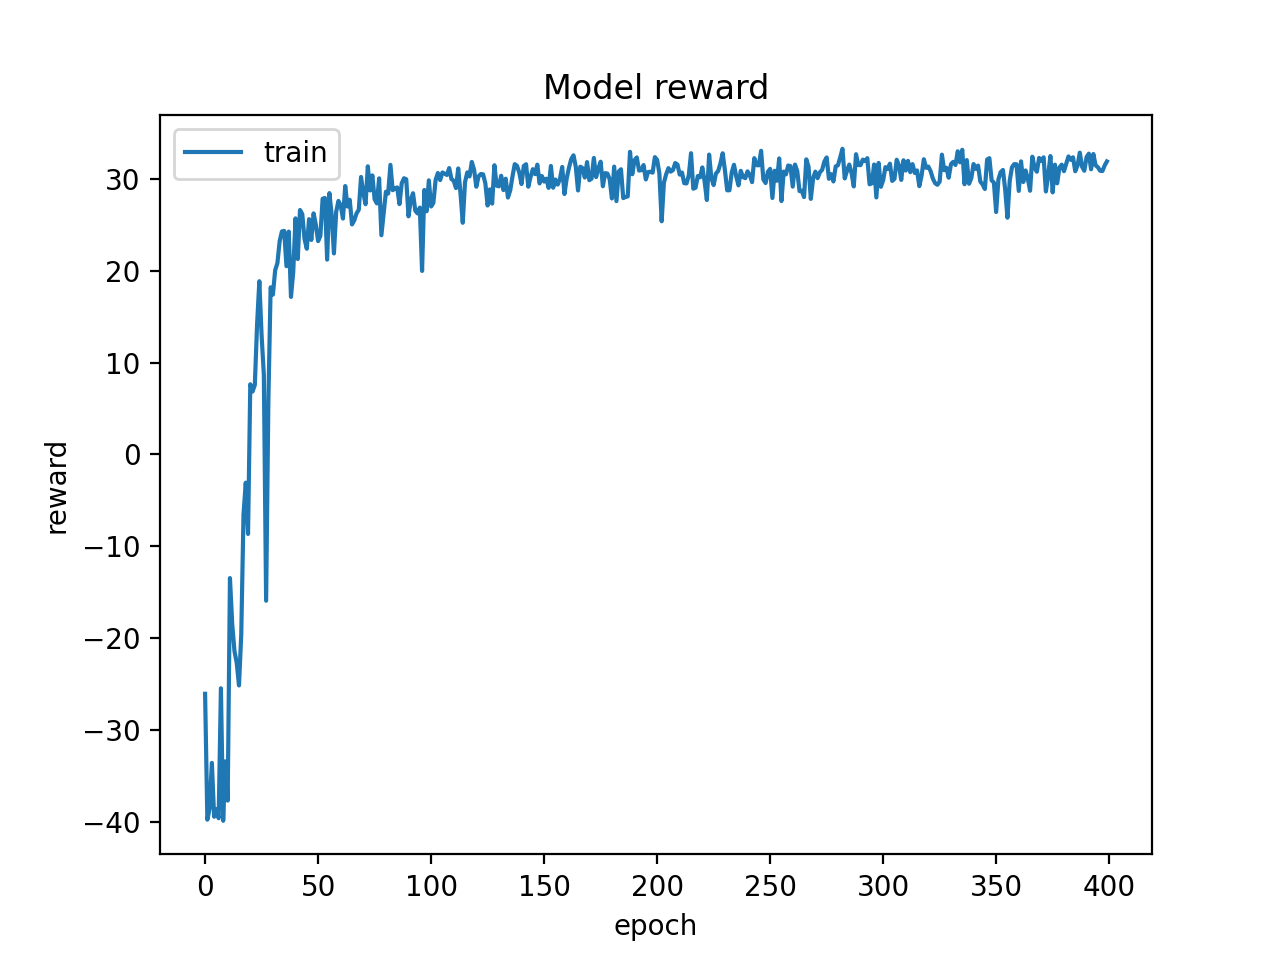
\includegraphics[scale=0.95]{chapter7/img/rewardtrain.png}
        \end{center}
        \caption{Biểu đồ đường cong huấn luyện cho phần thưởng}
        \label{fig:rewardtrain}
    \end{figure}
\end{center}

\subsubsection{Nhận xét}
Với kết quả biểu diễn ở hình \ref{fig:rewardtrain}, ta thấy:

\begin{itemize}
    \item Giai đoạn đầu, phần thưởng nhận được là cực thấp. Vì thời gian đầu, tác nhân cần được khám phá thị trường một cách tổng quát nhất.
    \item Tuy nhiên, để phần thưởng nhận được trở nên tích cực, nó chỉ mất khoảng 5000 đến 10000 lượt hội thoại.
    \item Độ dốc đường cong ở các epoch cuối là thấp, phần thưởng nhận được khá ổn định trong giai đoạn cuối của huấn luyện. Chứng tỏ, huấn luyện được mô hình có chính sách (policy) ổn định.
    \item Kết quả cuối huấn luyện của mô hình khá tốt. Phần thưởng giao động trên 30 điểm.
\end{itemize}

% Có ba số liệu thống kê của biểu đồ này quan trọng:
% • Độ dốc tiệm cận cho thấy chính sách tốt như thế nào sau khi thuật toán đã ổn định.
% • Mức tối thiểu của đường cong cho thấy phần thưởng phải được hy sinh trước khi nó bắt đầu cải thiện.
% • Việc vượt qua số 0 cho thấy phải mất bao lâu cho đến khi thuật toán thu hồi được chi phí học tập của nó.

Ngoài ra, ta còn có một biểu đồ đường cong huấn luyện biểu diễn tỉ lệ thành công của hội thoại như hình \ref{fig:successtrain}. Tỉ lệ thành công được tính của 100 lượt hội thoại.

\clearpage

\begin{center}
    \begin{figure}[ht!]
        \begin{center}
         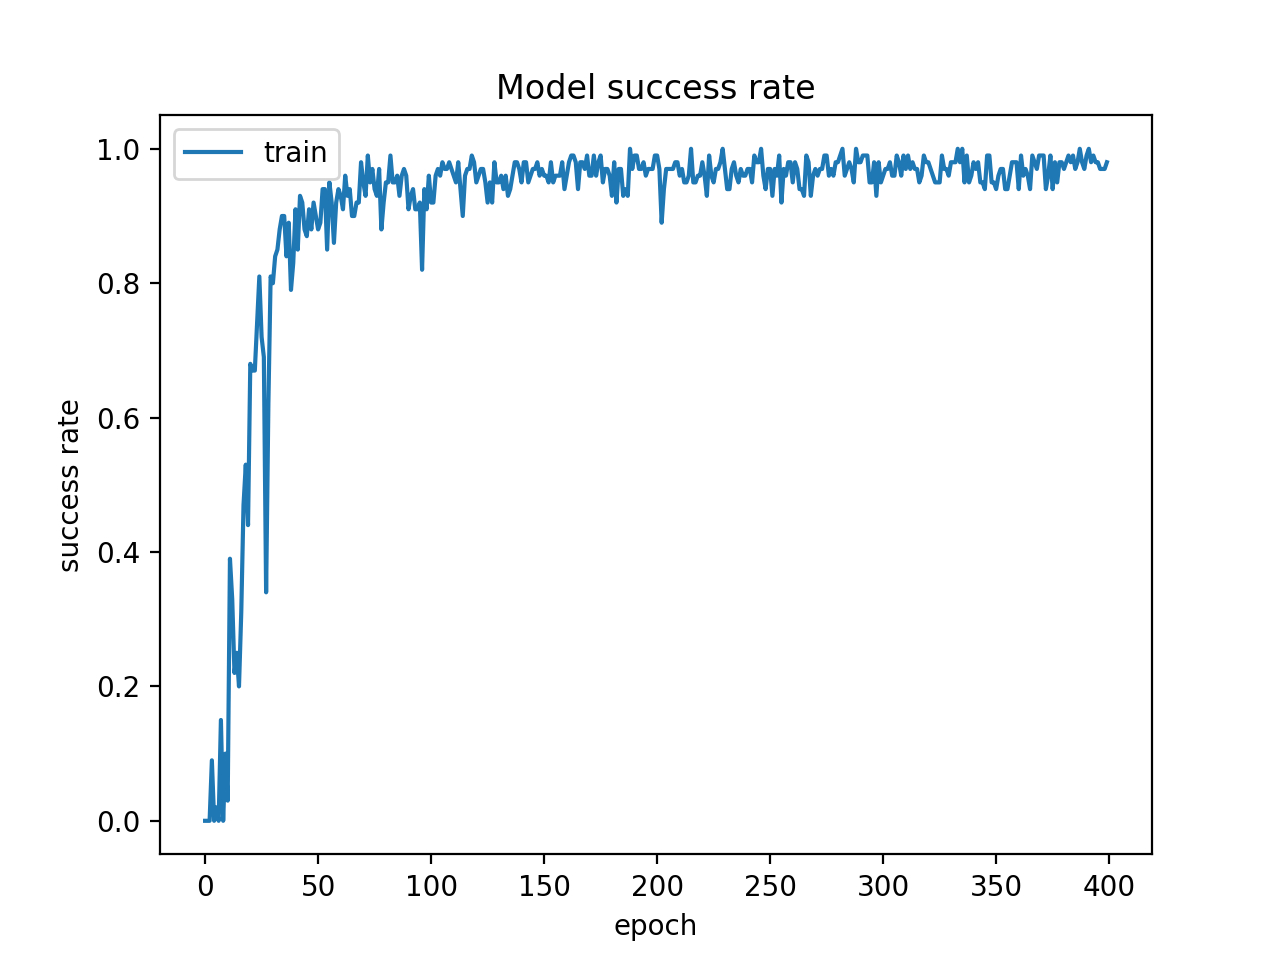
\includegraphics[scale=0.95]{chapter7/img/successtrain.png}
        \end{center}
        \caption{Biểu đồ đường cong huấn luyện cho tỉ lệ thành công}
        \label{fig:successtrain}
    \end{figure}
\end{center}

\subsubsection{Nhận xét}
Với kết quả biểu diễn ở hình \ref{fig:successtrain}, ta thấy:

\begin{itemize}
    \item Giai đoạn đầu, tỉ lệ thành công là cực thấp. Tương đương với phần thưởng nhận được thấp như mô tả ở hình \ref{fig:rewardtrain}.
    \item Tỉ lệ thành công cũng trở nên tốt hơn sau 5000 đến 10000 lượt hội thoại.
    \item Độ dốc đường cong ở các epoch cuối là thấp, tỉ lệ thành công khá ổn định trong giai đoạn cuối của huấn luyện.
    \item Kết quả cuối huấn luyện của mô hình khá tốt. Tỉ lệ thành công giao động từ 0.97 đến 1.
\end{itemize}

\subsection{Kiểm thử mô hình sử dụng bộ mô phỏng người dùng}
Như đã trình bày ở mục \ref{sec:usersim}, \textit{User Simulator} là bộ mô phỏng người dùng thật để tương tác với tác nhân. Sau khi huấn luyện, ta cũng có thể sử dụng nó để đánh giá mô hình. Việc dùng bộ mô phỏng người dùng cho việc đánh giá sẽ giảm thiểu thời gian và công sức rất nhiều so với người dùng thật. Ngoài ra, bằng cách chạy tự động và với tập dữ liệu mục tiêu người dùng, chúng ta đánh giá được mô hình với nhiều loại kịch bản khác nhau. 

Hệ thống để đánh giá mô hình tương tự như quá trình huấn luyện. Với bộ mô phỏng người dùng, ta chỉ đánh giá với tiêu chí là cuộc hội thoại có thành công hay không, cụ thể được mô tả như sau:

\subsubsection{Tiêu chí đánh giá}
Cuộc hội thoại kết thúc thành công khi:

\begin{itemize}
    \item Các thông tin mà tác nhân cung cấp không xung đột với các ràng buộc mà người dùng cung cấp.
    \item Hoàn thành đủ mục tiêu của người dùng, các thông tin mà người dùng yêu cầu được cung cấp đầy đủ bởi tác nhân.
    \item Tác nhân tìm thấy sản phẩm thỏa mãn mọi yêu cầu của người dùng. Mục tiêu cuối cùng của Chatbot này chốt được đơn hàng cho người dùng nên trong trường hợp tác nhân tìm thấy thông tin sản phẩm nhưng bị từ chối bởi người dùng vẫn tính là không thành công.
\end{itemize}

\subsubsection{Kết quả}
Sử dụng tập mục tiêu người dùng (User Goal) như mô tả ở mục \ref{subsec:usergoal}, sau 10000 cuộc hội thoại diễn ra, ta đạt được xác suất \textbf{96\%} cuộc hội thoại thành công. 

\subsubsection{Nhận xét}
Với kết quả 96\% cuộc hội thoại thành công, tác nhân đã gần như lúc nào cũng hoàn thành được nhu cầu của người dùng. Sau khi phân tích cụ thể các trường hợp không thành công, đa phần đến từ việc tư vấn kích cỡ sản phẩm phù hợp cho người dùng. Nguyên nhân do dữ liệu về kích cỡ cơ thể chưa đủ phong phú để tìm được kích cỡ phù hợp, và một phần do số đo cơ thể người dùng thực sự không phù hợp cho các sản phẩm mà cửa hàng kinh doanh.

\subsection{Đánh giá từ người dùng thực}
Để nhận đánh giá từ người dùng một cách nhanh chóng và rõ ràng, trong luận án này, xây dựng một bộ các câu hội thoại/ đoạn hội thoại, gửi cho một số người dùng thực tế để đánh giá. Ngoài ra, thực hiện so sánh với một ứng dụng Chatbot tư vấn tương tự khác. Chatbot này không huấn luyện mô hình mà chỉ thực hiện theo một bộ luật định sẵn (Chatbot rule-based). Việc này nhằm mục đích so sánh Chatbot huấn luyện theo mô hình học tăng cường đạt được mục tiêu ứng dụng thực tế nhất định.

\subsubsection{Tiêu chí đánh giá}
Các tiêu chí đánh giá cho các câu thoại bao gồm:

\begin{itemize}
    \item Thỏa mãn yêu cầu người dùng đưa ra
    \item Tính hợp lý, thiết thực của các câu yêu cầu từ tác nhân
    \item Tính tự nhiên, dễ trả lời của các câu yêu cầu từ tác nhân
    \item Tính thiết thực, hữu ích của các thông tin mà tác nhân cung cấp
    \item Tính chính xác của các thông tin mà tác nhân cung cấp
\end{itemize}

Các tiêu chí đánh giá cho toàn bộ hội thoại bao gồm:

\begin{itemize}
    \item Mức độ đáp ứng nhu cầu tư vấn sản phẩm nói chung
    \item Mức độ giao tiếp tự nhiên trong suốt cuộc hội thoại
    \item Đánh giá tổng quan của người dùng
\end{itemize}

Toàn bộ các tiêu chí này sẽ được đánh giá thêm một cột rằng nó có tốt hơn so với \textit{Chatbot rule-based} hay không.

\subsubsection{Nội dung đánh giá}
Các câu thoại tạo ra để mang đi đánh giá nên thể hiện tất cả các trường hợp khi người dùng tham dự vào hội thoại. Cụ thể:

Nội dung đánh giá cho các câu thoại thông thường:

\begin{itemize}
    \item Chào hỏi với tác nhân gồm: 
    \begin{itemize}
        \item Chào hỏi khi bắt đầu cuộc hội thoại
        \item Chào hỏi ở giữa cuộc hội thoại
        \item Chào hỏi khi kết thúc cuộc hội thoại
        \item Chào hỏi nhiều lần
    \end{itemize}
    \item Cám ơn/tạm biệt với tác nhân gồm: 
    \begin{itemize}
        \item Khách hàng cám ơn shop sau khi xác nhận đặt hàng, được tư vấn sản phẩm
        \item Khách hàng cám ơn shop sau khi nhận được thông tin sản phẩm hữu ích
        \item Khách hàng cám ơn ở những trường hợp không liên quan khác
        \item Cám ơn nhiều lần
    \end{itemize}
    \item Khác: Khách hàng hỏi các thông tin khác không liên quan tới tư vấn sản phẩm
\end{itemize}

Tiêu chí đánh giá cho các câu thoại thông thường:

\begin{itemize}
    \item Tính hợp lý: Không hợp lý, phải cải thiện -> Không hợp lý lắm, nhưng chấp nhận được -> Hợp lý
    \item Tính tự nhiên: Không tự nhiên, phải cải thiện -> Không tự nhiên lắm, nhưng chấp nhận được -> Tự nhiên
    \item Tính hợp lý/ Tính tự nhiên so với \textit{Chatbot rule-based}: Tệ hơn -> Như nhau -> Tốt hơn
\end{itemize}

Nội dung đánh giá cho các câu thoại tư vấn:

\begin{itemize}
    \item Yêu cầu cung cấp thông tin sản phẩm. Trường hợp có hàng và không có hàng gồm:
    \begin{itemize}
        \item Gửi tên sản phẩm, hỏi đơn giá
        \item Gửi tên sản phẩm, hỏi màu sản phẩm
        \item Gửi tên sản phẩm, hỏi chất liệu sản phẩm
        \item Gửi tên sản phẩm, hỏi kích cỡ sản phẩm
        \item Gửi tên sản phẩm, kích cỡ, hỏi đơn giá
        \item Gửi tên sản phẩm, màu, hỏi đơn giá
        \item Gửi tên sản phẩm, kích cỡ, hỏi màu sản phẩm
        \item Gửi tên sản phẩm, màu, hỏi chất liệu sản phẩm
        \item Gửi tên sản phẩm, kích cỡ, hỏi chất liệu sản phẩm
        \item Gửi tên sản phẩm, màu, hỏi kích cỡ sản phẩm
        \item Gửi tên sản phẩm, hỏi còn hàng hay không
        \item Gửi tên sản phẩm, màu, hỏi còn hàng hay không
        \item Gửi tên sản phẩm, kích cỡ, hỏi còn hàng hay không
        \item Gửi tên sản phẩm, màu, kích cỡ, hỏi còn hàng hay không
    \end{itemize}
    \item Tư vấn chọn kích cỡ:
    \begin{itemize}
        \item Chỉ gửi chiều cao
        \item Chỉ nhập cân nặng
        \item Chỉ gửi vòng eo
        \item Gửi chiều cao, cân nặng
        \item Gửi chiều cao, vòng eo
        \item Gửi vòng eo, cân nặng
        \item Gửi chiều cao, cân nặng, vòng eo. Trường hợp có kích cỡ phù hợp 
        \item Gửi chiều cao, cân nặng, vòng eo. Trường hợp không có kích cỡ phù hợp
    \end{itemize}
    \item Đặt hàng:
    \begin{itemize}
        \item Chỉ gửi tên sản phẩm
        \item Chỉ gửi màu sản phẩm
        \item Chỉ gửi kích cỡ sản phẩm
        \item Chỉ gửi số lượng sản phẩm
        \item Gửi màu, số lượng sản phẩm
        \item Gửi màu, kích cỡ sản phẩm
        \item Gửi kích cỡ, số lượng sản phẩm
        \item Gửi tên sản phẩm, màu
        \item Gửi tên sản phẩm, kích cỡ
        \item Gửi tên sản phẩm, số lượng
        \item Gửi tên sản phẩm, màu, kích cỡ
        \item Gửi tên sản phẩm, màu, số lượng
        \item Gửi tên sản phẩm, kích cỡ, số lượng
        \item Gửi tên sản phẩm, màu, kích cỡ, số lượng
    \end{itemize}
\end{itemize}

Tiêu chí đánh giá cho các câu thoại tư vấn:

\begin{itemize}
    \item Thỏa mãn yêu cầu người dùng đưa ra: Không thỏa mãn -> Chấp nhận được -> Thỏa mãn
    \item Tính hợp lý, thiết thực: Không hợp lý, phải cải thiện -> Không hợp lý lắm, nhưng chấp nhận được -> Hợp lý
    \item Tính tự nhiên, dễ trả lời: Không tự nhiên, phải cải thiện -> Không tự nhiên lắm, nhưng chấp nhận được -> Tự nhiên
    \item Tính thiết thực, hữu ích: Không thiết thực -> Chấp nhận được -> Thiết thực
    \item Tính chính xác: Không chính xác -> Chấp nhận được -> Chính xác
    \item So sánh với \textit{Chatbot rule-based} các tiêu chí trên: Tệ hơn -> Như nhau -> Tốt hơn
\end{itemize}

Nội dung đánh giá cho các hội thoại:

\begin{itemize}
    \item Hội thoại hỏi các thông tin của sản phẩm và chốt đơn hàng
    \item Hội thoại hỏi sản phẩm, mà cửa hàng không bán hoặc đã hết
    \item Hội thoại hỏi các thông tin của sản phẩm. Trường hợp các thông tin không tìm thấy sản phẩm phù hợp
    \item Tư vấn kích cỡ sản phẩm phù hợp với khách hàng
    \item Tư vấn kích cỡ sản phẩm phù hợp với khách hàng. Trường hợp không có kích cỡ thích hợp
    \item Thay đổi sản phẩm sau khi đặt hàng
\end{itemize}

Tiêu chí đánh giá cho các hội thoại:

\begin{itemize}
    \item Mức độ đáp ứng nhu cầu tư vấn sản phẩm nói chung: đánh giá 5 mức độ từ chưa đáp ứng đến rất đầy đủ
    \item Mức độ giao tiếp tự nhiên: đánh giá 5 mức độ từ không tự nhiên đến rất tự nhiên
    \item Đánh giá tổng quan: với mức điểm từ một sao đến 5 sao
    \item So sánh với \textit{Chatbot rule-based} các tiêu chí trên: Tệ hơn -> Như nhau -> Tốt hơn
\end{itemize}

\subsubsection{Kết quả đánh giá}
\subsubsection{Tiêu chí thỏa mãn yêu cầu người dùng đưa ra}
Hình \ref{fig:tieuchi1} mô tả kết quả đánh giá của người dùng cho tiêu chí thỏa mãn yêu cầu người dùng đưa ra khi Chatbot trả về kết quả.

\begin{center}
    \begin{figure}[ht!]
        \begin{center}
         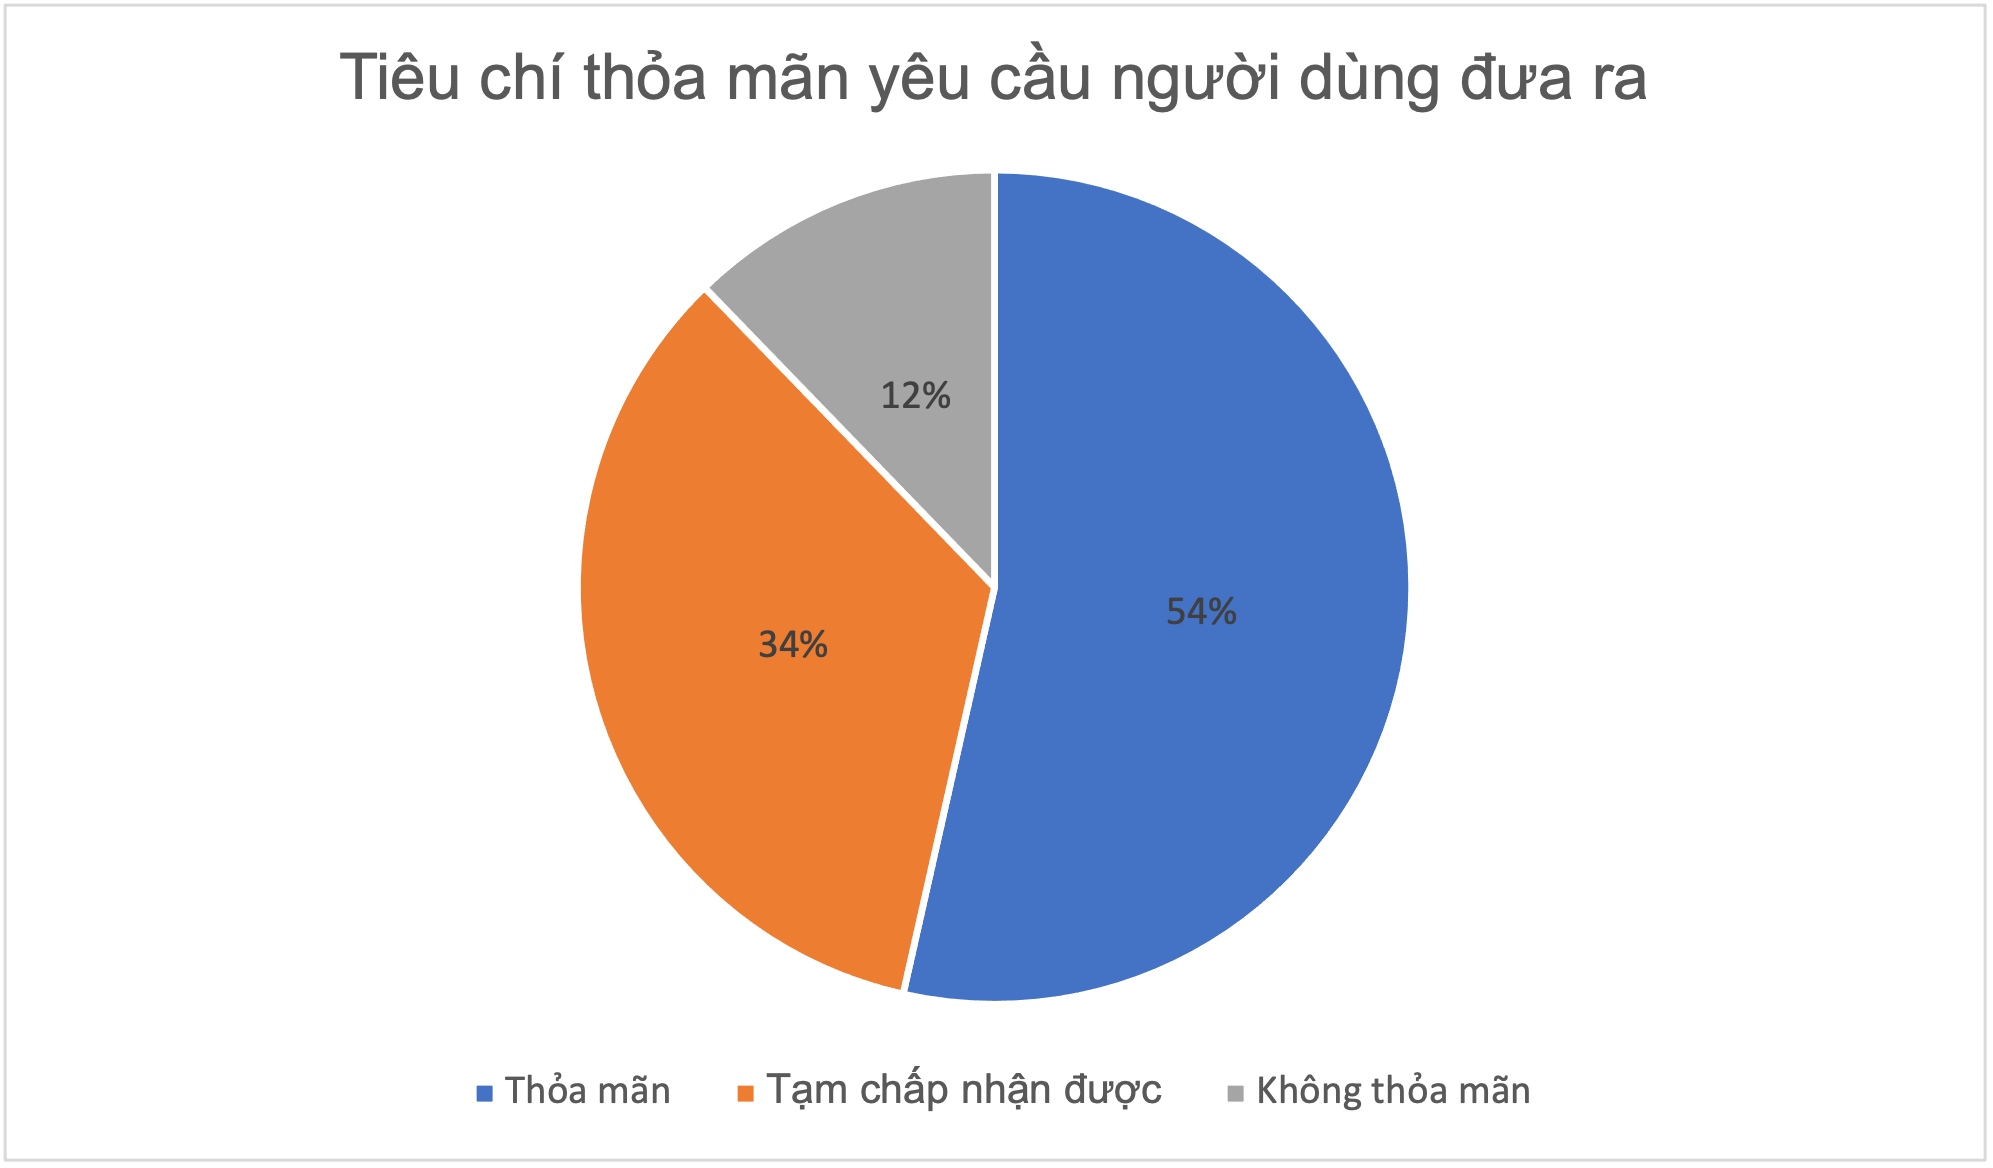
\includegraphics[scale=0.91]{chapter7/img/tieuchi1.png}
        \end{center}
        \caption{Kết quả đánh giá tiêu chí thỏa mãn yêu cầu người dùng}
        \label{fig:tieuchi1}
    \end{figure}
\end{center}

\textbf{Nhận xét:}
Có 88\% nhận xét từ tạm chấp nhận được cho đến thỏa mãn hết các yêu cầu. Trong đó hơn 50\% là thỏa mãn. Chỉ có 12\% nhận xét là không thỏa mãn. Sau khi phân tích cụ thể các kết quả đánh giá không thỏa mãn, nhận thấy các đánh giá này đa phần đến từ khi người dùng yêu cầu một thông tin nào đó của sản phẩm không tồn tại trong cơ sở dữ liệu (cửa hàng không bán hoặc hết hàng) và không cung cấp được thông tin họ yêu cầu.

\subsubsection{So sánh với Chatbot rule-based}
Hình \ref{fig:tieuchi12} mô tả kết quả đánh giá của người dùng khi so sánh tiêu chí thỏa mãn yêu cầu người dùng đưa ra với Chatbot rule-based.

\begin{center}
    \begin{figure}[ht!]
        \begin{center}
         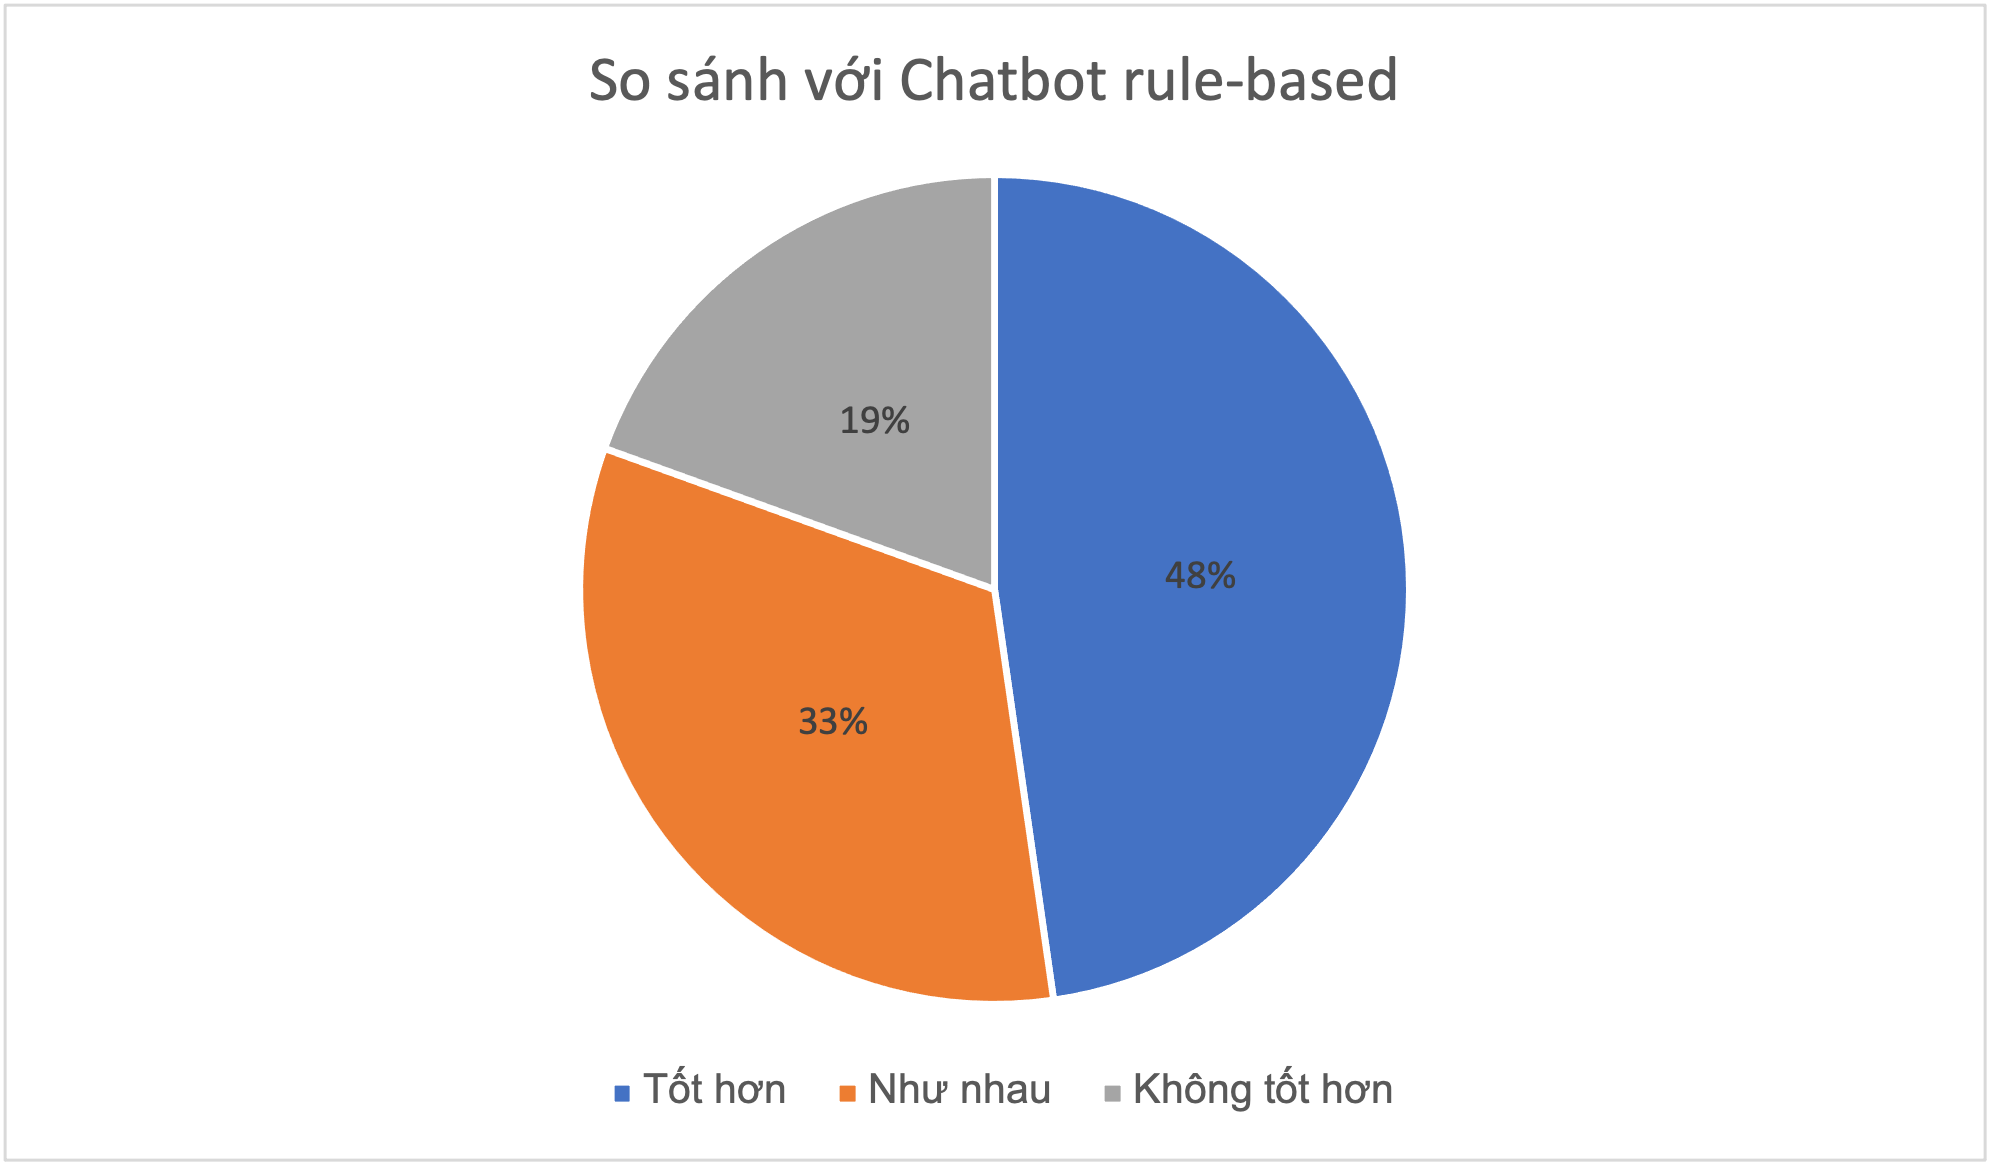
\includegraphics[scale=0.91]{chapter7/img/tieuchi1_2.png}
        \end{center}
        \caption{Kết quả so sánh với Chatbot rule-based}
        \label{fig:tieuchi12}
    \end{figure}
\end{center}

\textbf{Nhận xét:}
Có hơn 80\% đánh giá là tốt hơn hoặc tương đương với Chatbot rule-based. Có 19\% là không tốt hơn. Sau khi phân tích cụ thể các kết quả đánh giá không tốt, nhận thấy Chatbot rule-based này sẽ liệt kê tất cả thông tin của sản phẩm trong lượt đầu. Việc này thỏa mãn một số người dùng tốt hơn Chatbot khi sử dụng học tăng cường.

\subsubsection{Tiêu chí về tính hợp lý, thiết thực của các câu yêu cầu từ tác nhân}
Hình \ref{fig:tieuchi2} mô tả kết quả đánh giá của người dùng cho tiêu chí tính hợp lý, thiết thực của các câu yêu cầu từ tác nhân.

\begin{center}
    \begin{figure}[h!]
        \begin{center}
         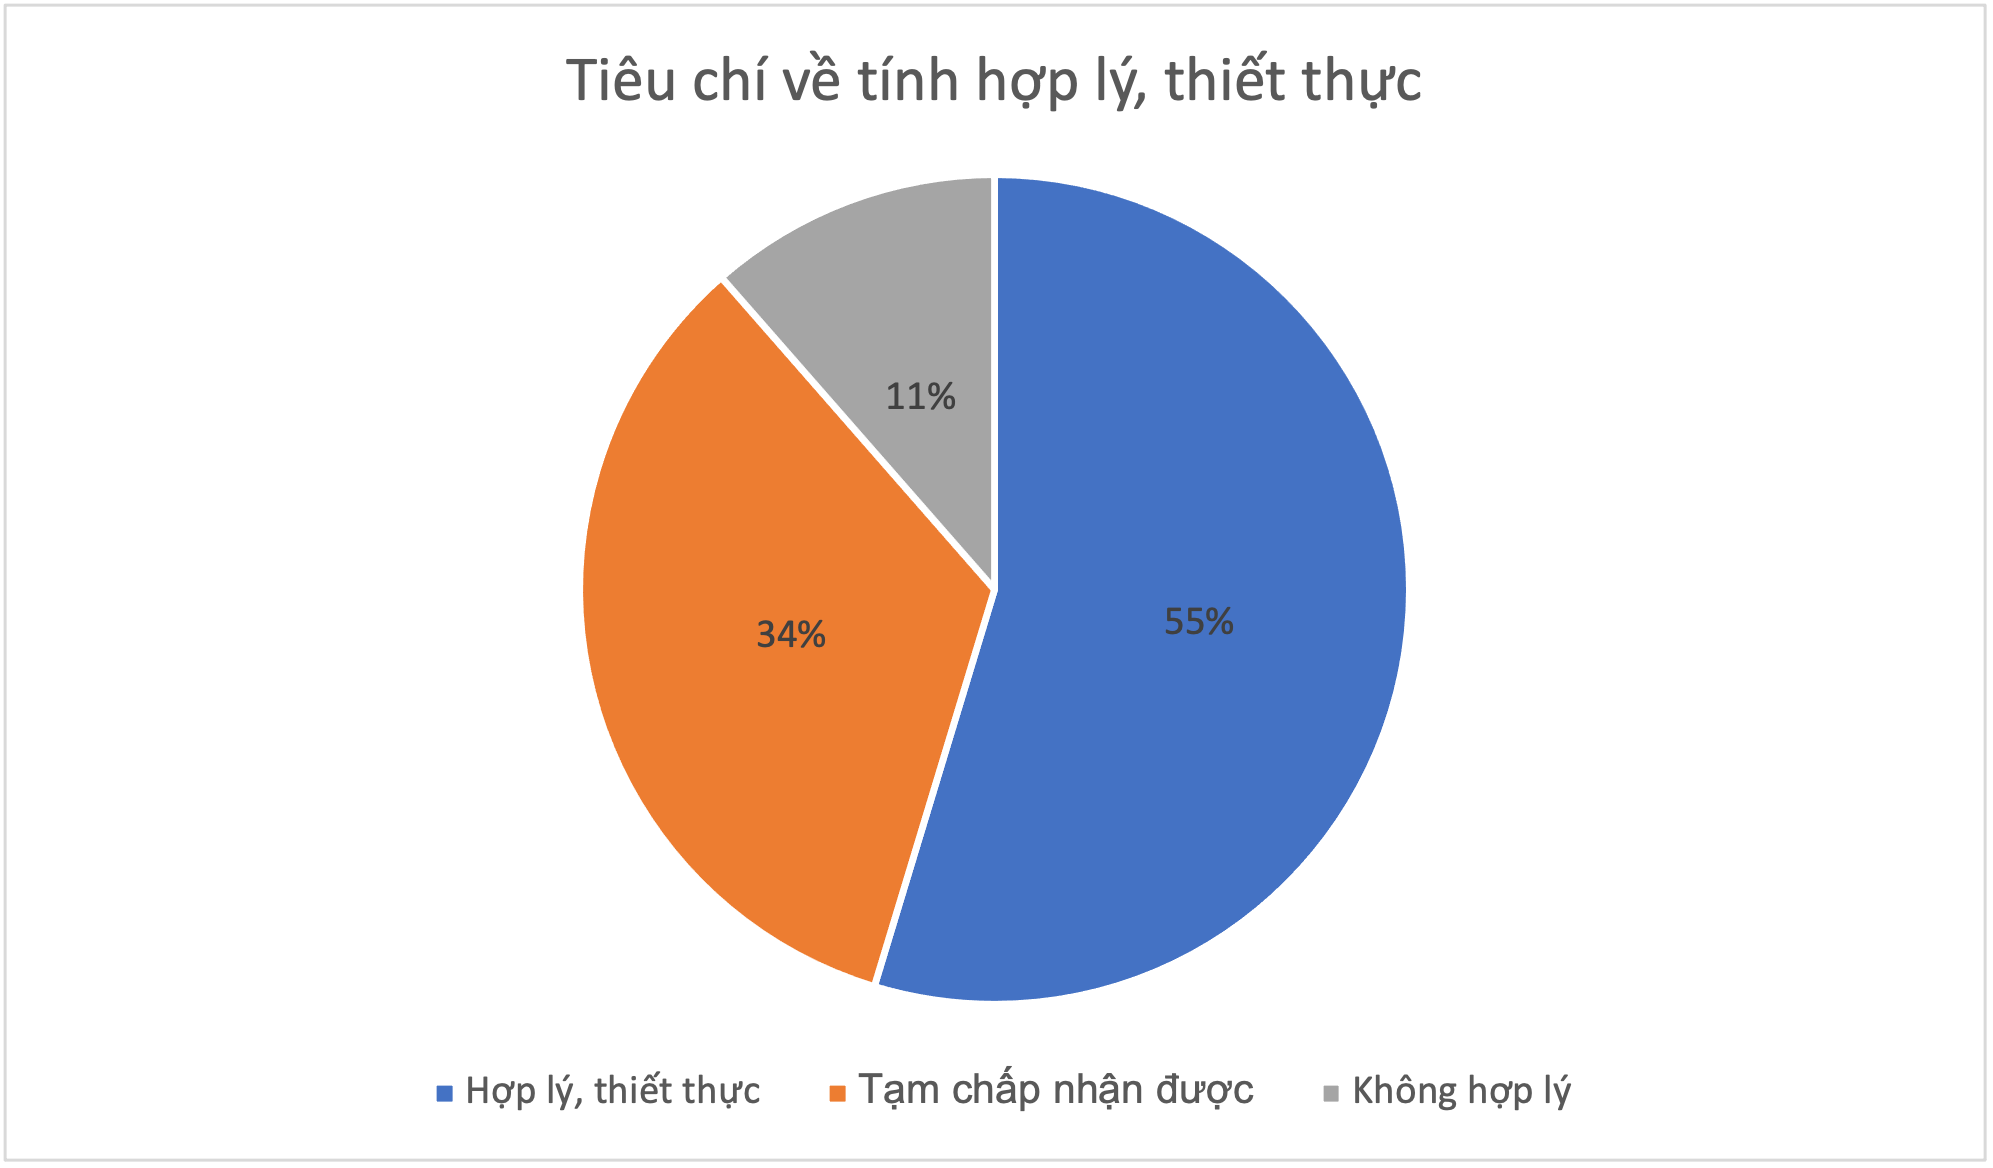
\includegraphics[scale=0.91]{chapter7/img/tieuchi2.png}
        \end{center}
        \caption{Kết quả đánh giá tiêu chí tính hợp lý, thiết thực}
        \label{fig:tieuchi2}
    \end{figure}
\end{center}

\textbf{Nhận xét:}
Có gần 90\% nhận xét từ tạm chấp nhận được cho đến hợp lý. Trong đó hơn 50\% là hợp lý. Chỉ có 11\% nhận xét là không hợp lý. Sau khi phân tích cụ thể các kết quả đánh giá không hợp lý, nhận thấy các đánh giá này đa phần đến từ khi người dùng yêu cầu một thông tin nào đó của sản phẩm, họ mong muốn Chatbot mau chóng trả lời thông tin mà họ cần thay vì phải trải qua một số các câu thoại yêu cầu khác trước khi trả về kết quả.

\subsubsection{So sánh với Chatbot rule-based}
Hình \ref{fig:tieuchi22} mô tả kết quả đánh giá của người dùng khi so sánh tiêu chí tính hợp lý, thiết thực với Chatbot rule-based.

\begin{center}
    \begin{figure}[h!]
        \begin{center}
         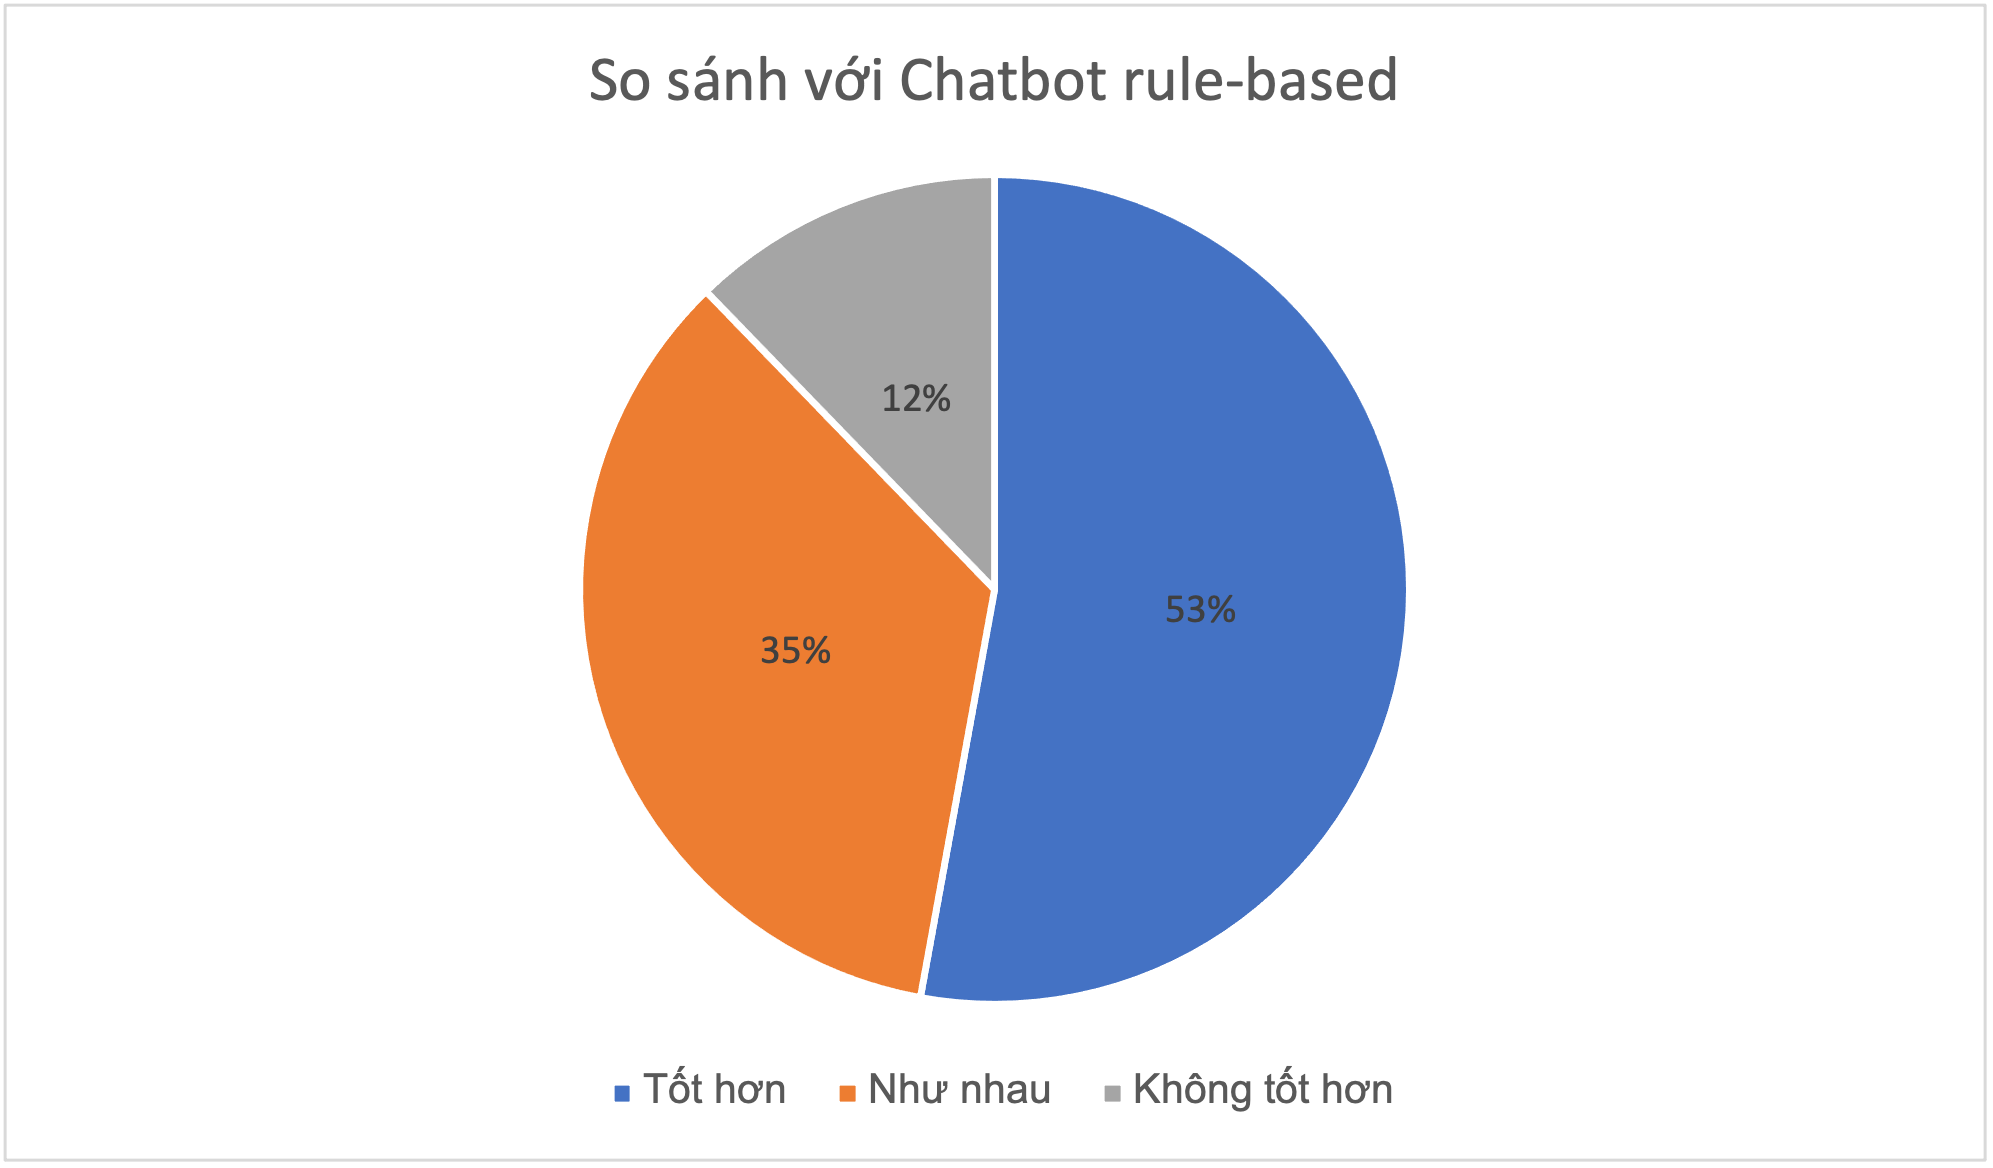
\includegraphics[scale=0.91]{chapter7/img/tieuchi2_2.png}
        \end{center}
        \caption{Kết quả so sánh với Chatbot rule-based}
        \label{fig:tieuchi22}
    \end{figure}
\end{center}

\textbf{Nhận xét:}
Có gần 90\% đánh giá là tốt hơn hoặc tương đương với Chatbot rule-based. Có 12\% là không tốt hơn. Sau khi phân tích cụ thể các kết quả đánh giá không tốt, nhận thấy tương tự với lí do trên, Chatbot rule-based này sẽ liệt kê tất cả thông tin của sản phẩm trong lượt đầu. Việc này thỏa mãn một số người dùng tốt hơn Chatbot khi sử dụng học tăng cường.

\subsubsection{Tiêu chí về tính tự nhiên, dễ trả lời của các câu yêu cầu từ tác nhân}
Hình \ref{fig:tieuchi3} mô tả kết quả đánh giá của người dùng cho tiêu chí tính tự nhiên, dễ trả lời của các câu yêu cầu từ tác nhân.

\begin{center}
    \begin{figure}[h!]
        \begin{center}
         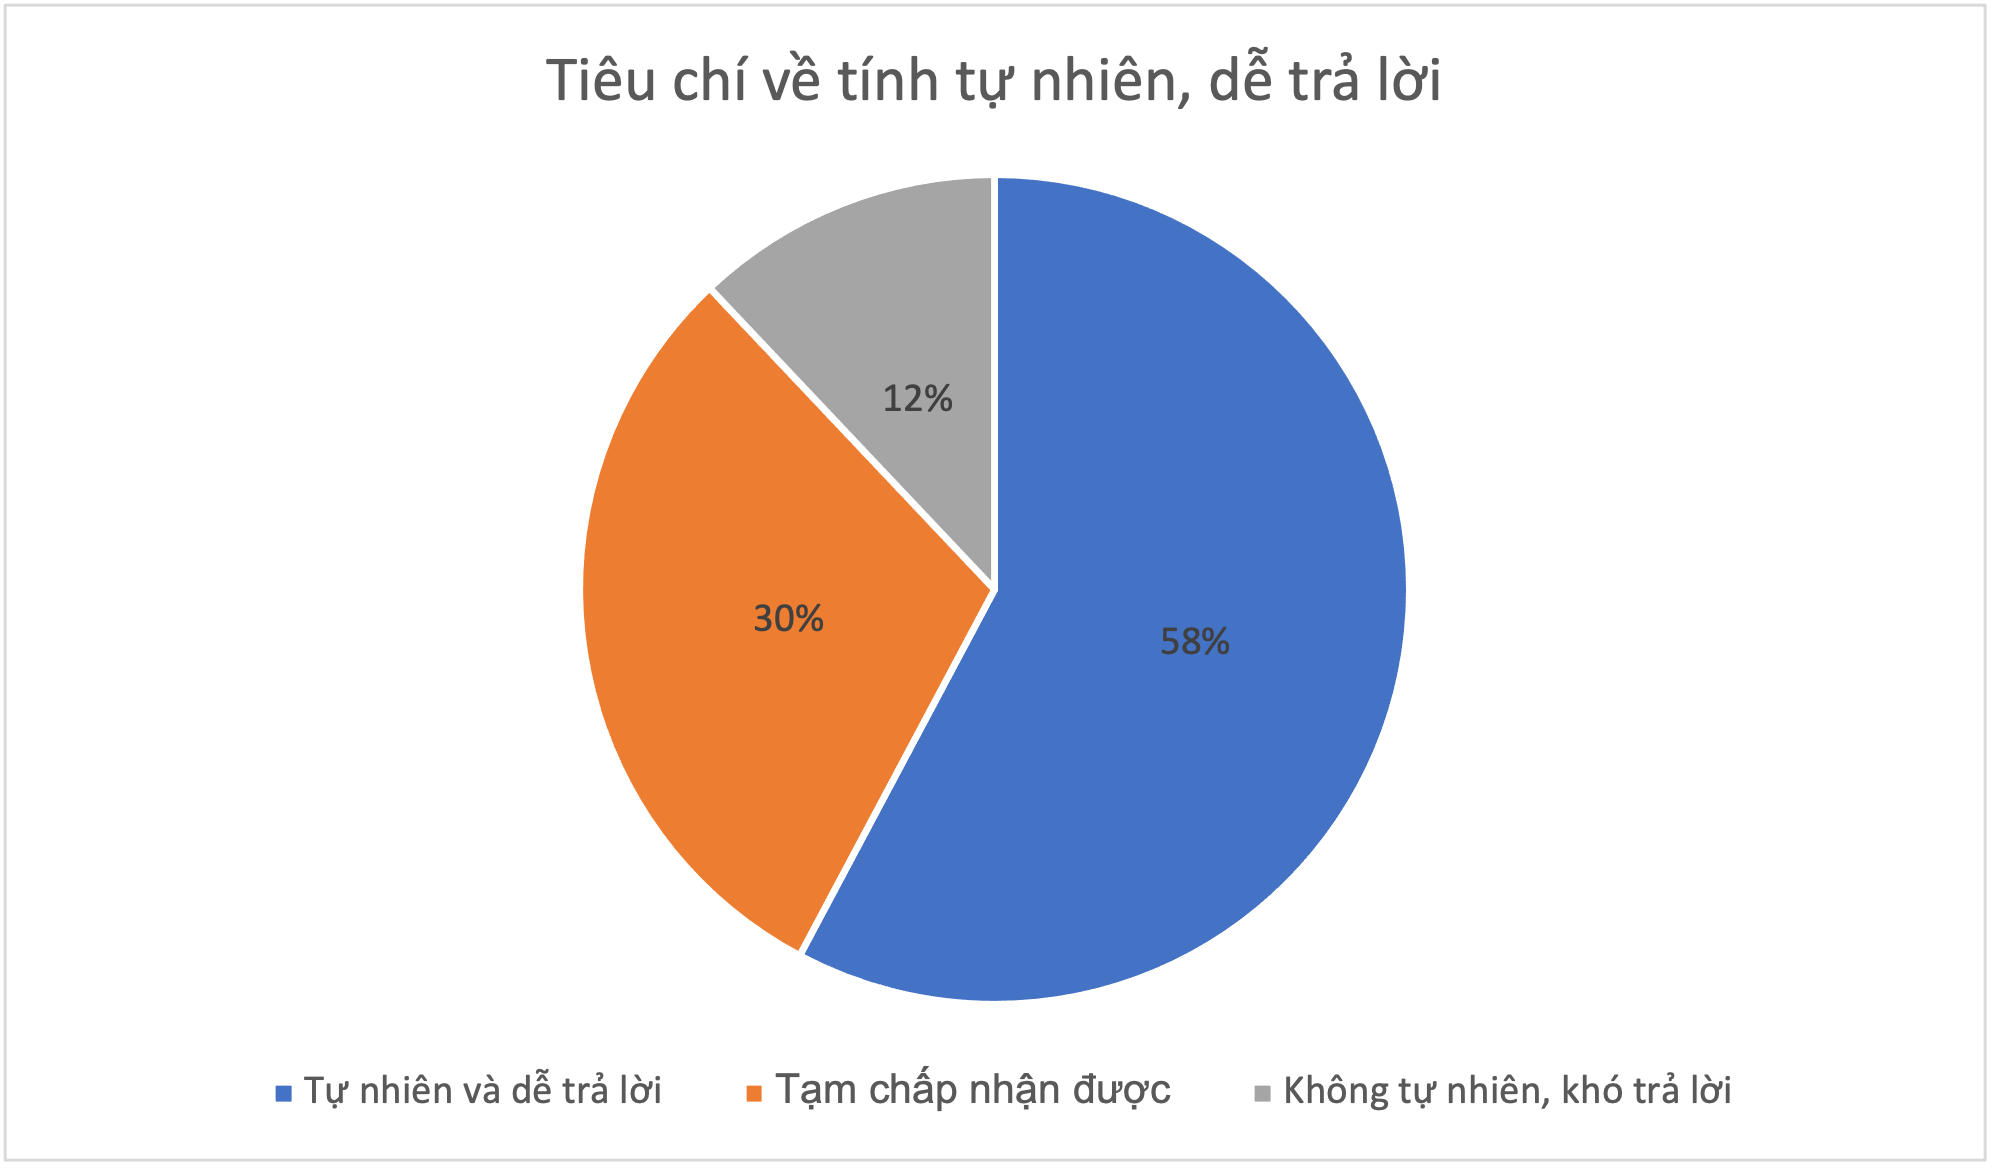
\includegraphics[scale=0.91]{chapter7/img/tieuchi3.png}
        \end{center}
        \caption{Kết quả đánh giá tiêu chí tính tự nhiên, dễ trả lời}
        \label{fig:tieuchi3}
    \end{figure}
\end{center}

\textbf{Nhận xét:}
Có gần 90\% nhận xét từ tạm chấp nhận được cho đến tự nhiên. Trong đó hơn 50\% là tự nhiên. Chỉ có 12\% nhận xét là không tự nhiên. Sau khi phân tích cụ thể các kết quả đánh giá không tự nhiên, nhận thấy các đánh giá này có thể đến từ bộ sinh phản hồi chưa phù hợp, dẫn tới các câu gây khó hiểu hoặc hiểu nhầm.

\subsubsection{So sánh với Chatbot rule-based}
Hình \ref{fig:tieuchi32} mô tả kết quả đánh giá của người dùng khi so sánh tiêu chí tính tự nhiên, dễ trả lời với Chatbot rule-based.

\begin{center}
    \begin{figure}[h!]
        \begin{center}
         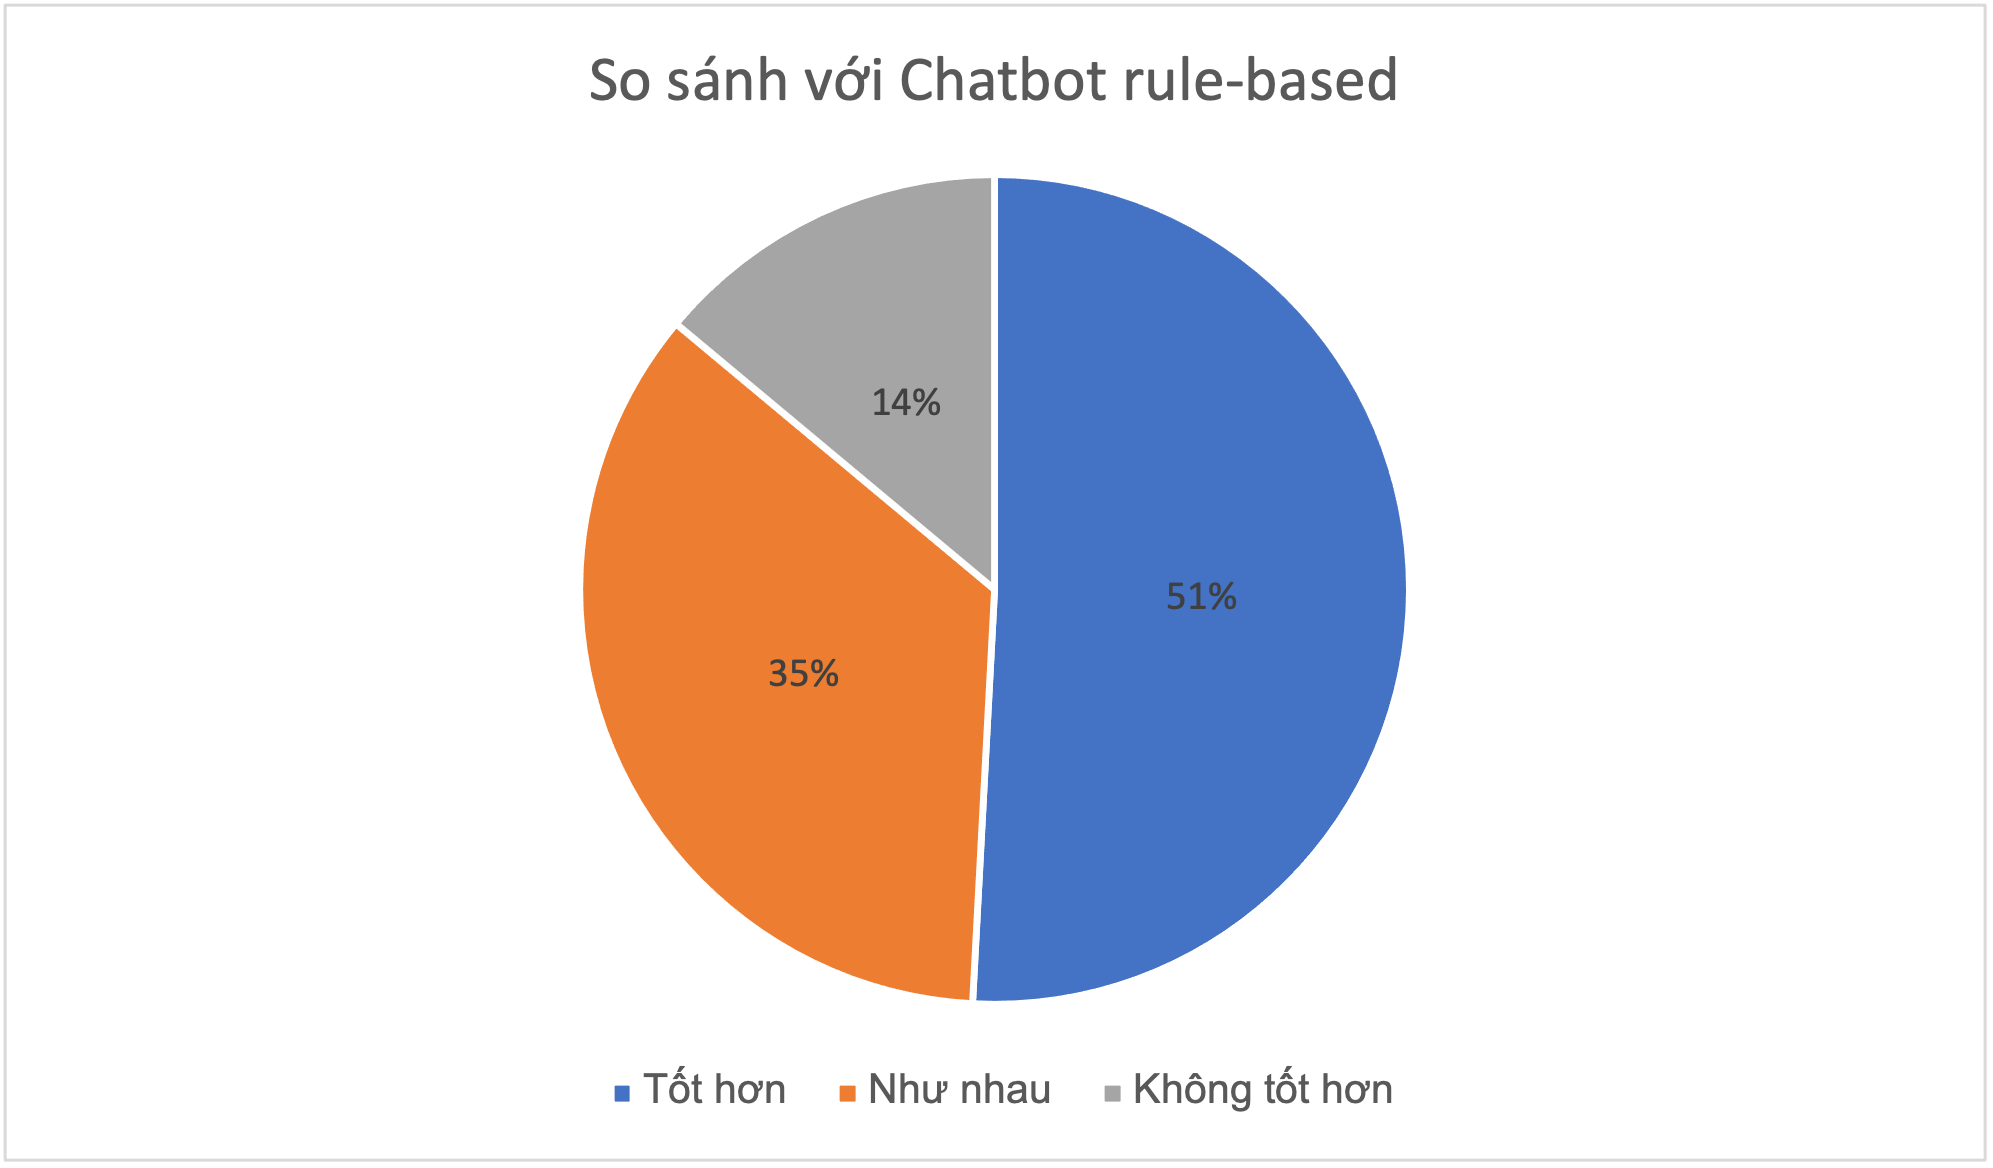
\includegraphics[scale=0.91]{chapter7/img/tieuchi3_2.png}
        \end{center}
        \caption{Kết quả so sánh với Chatbot rule-based}
        \label{fig:tieuchi32}
    \end{figure}
\end{center}

\textbf{Nhận xét:}
Có gần 90\% đánh giá là tốt hơn hoặc tương đương với Chatbot rule-based. Có 14\% là không tốt hơn. Sau khi phân tích cụ thể các kết quả đánh giá không tốt, nhận thấy tương tự với lí do trên, Chatbot rule-based này sinh câu phản hồi mà thỏa mãn một số người dùng tốt hơn Chatbot được xây dựng trong đề tài.

\subsubsection{Tiêu chí về tính thiết thực, hữu ích của các thông tin mà tác nhân cung cấp}
Hình \ref{fig:tieuchi4} mô tả kết quả đánh giá của người dùng cho tiêu chí tính thiết thực, hữu ích của các thông tin mà tác nhân cung cấp.

\begin{center}
    \begin{figure}[h!]
        \begin{center}
         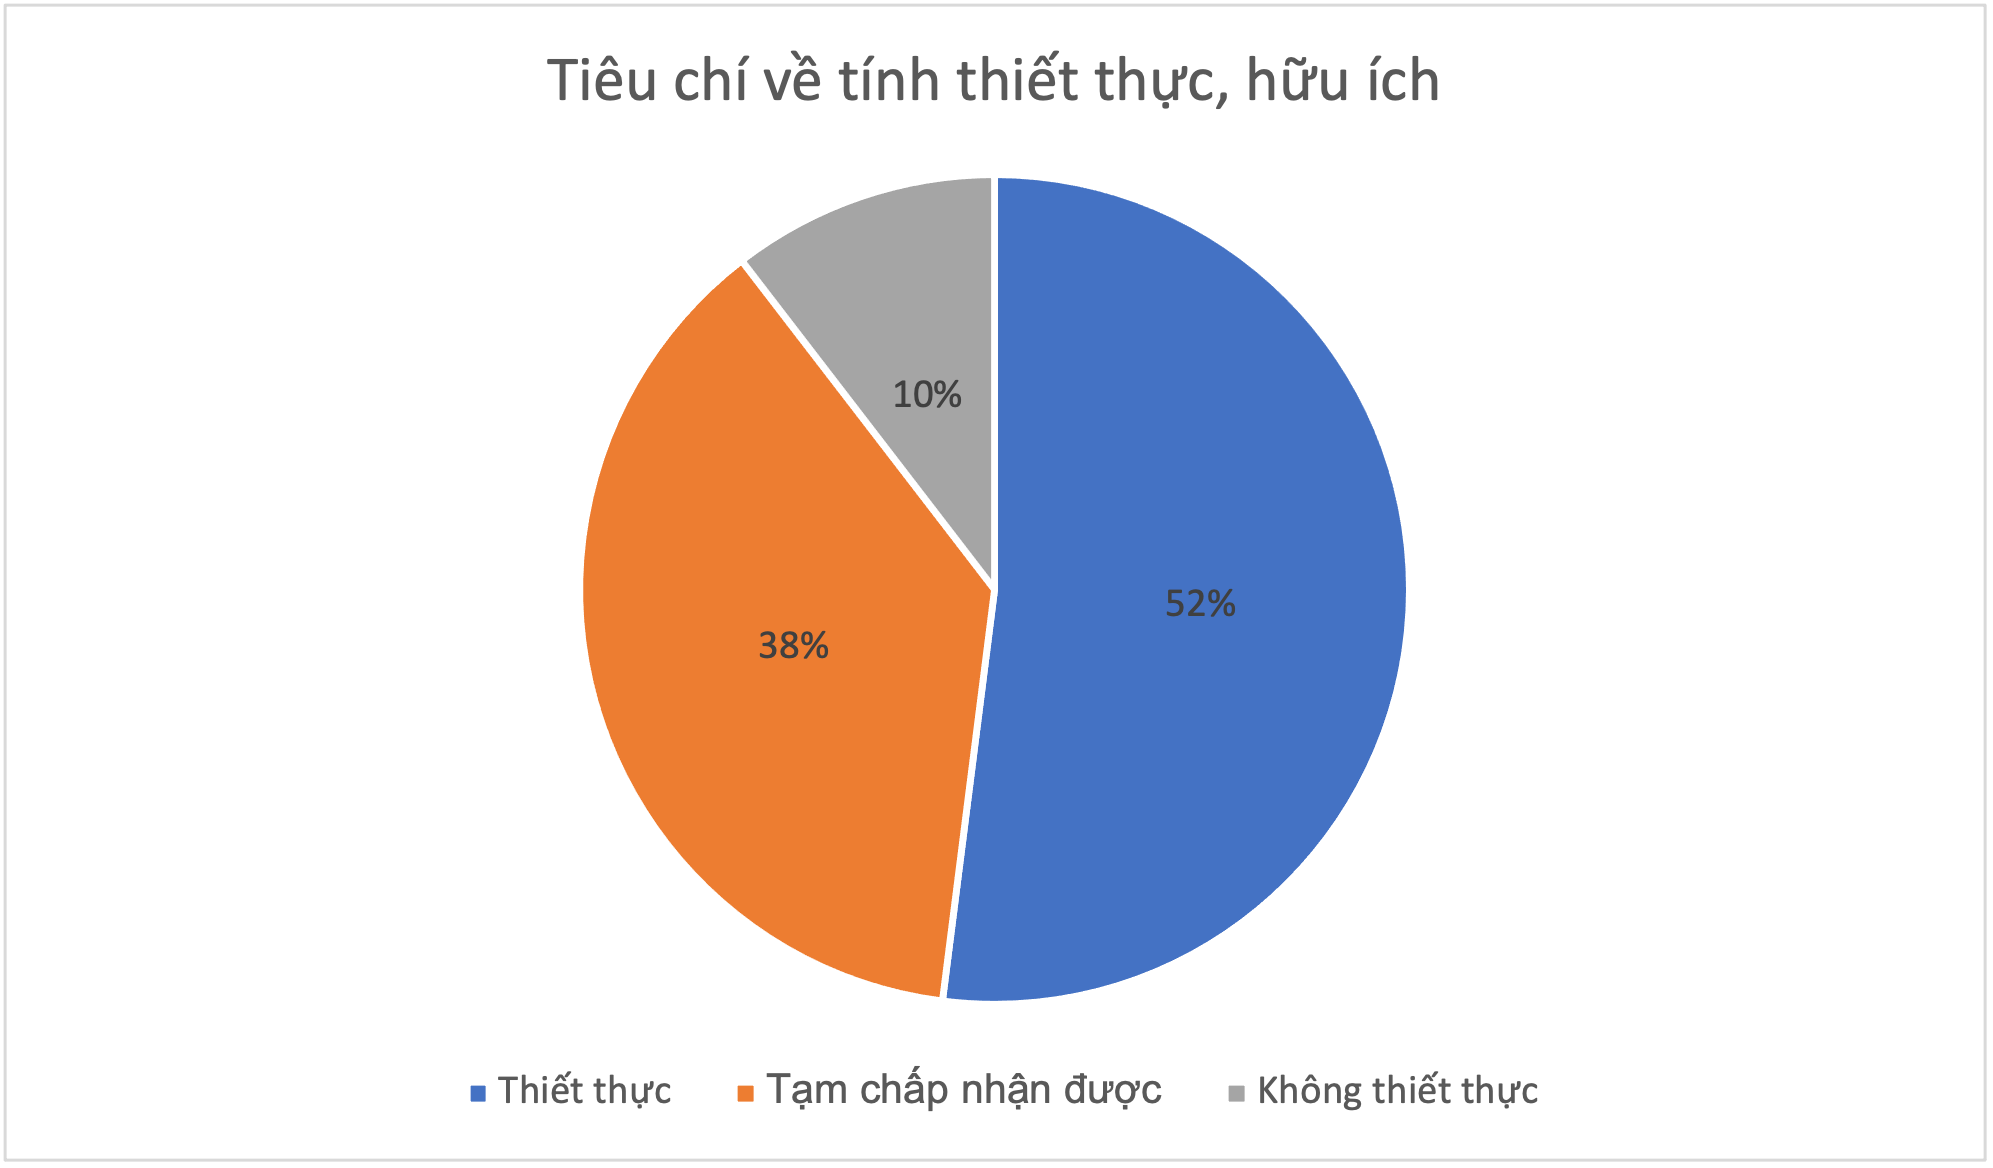
\includegraphics[scale=0.91]{chapter7/img/tieuchi4.png}
        \end{center}
        \caption{Kết quả đánh giá tiêu chí tính thiết thực, hữu ích}
        \label{fig:tieuchi4}
    \end{figure}
\end{center}

\begin{center}
    \begin{figure}[h!]
        \begin{center}
         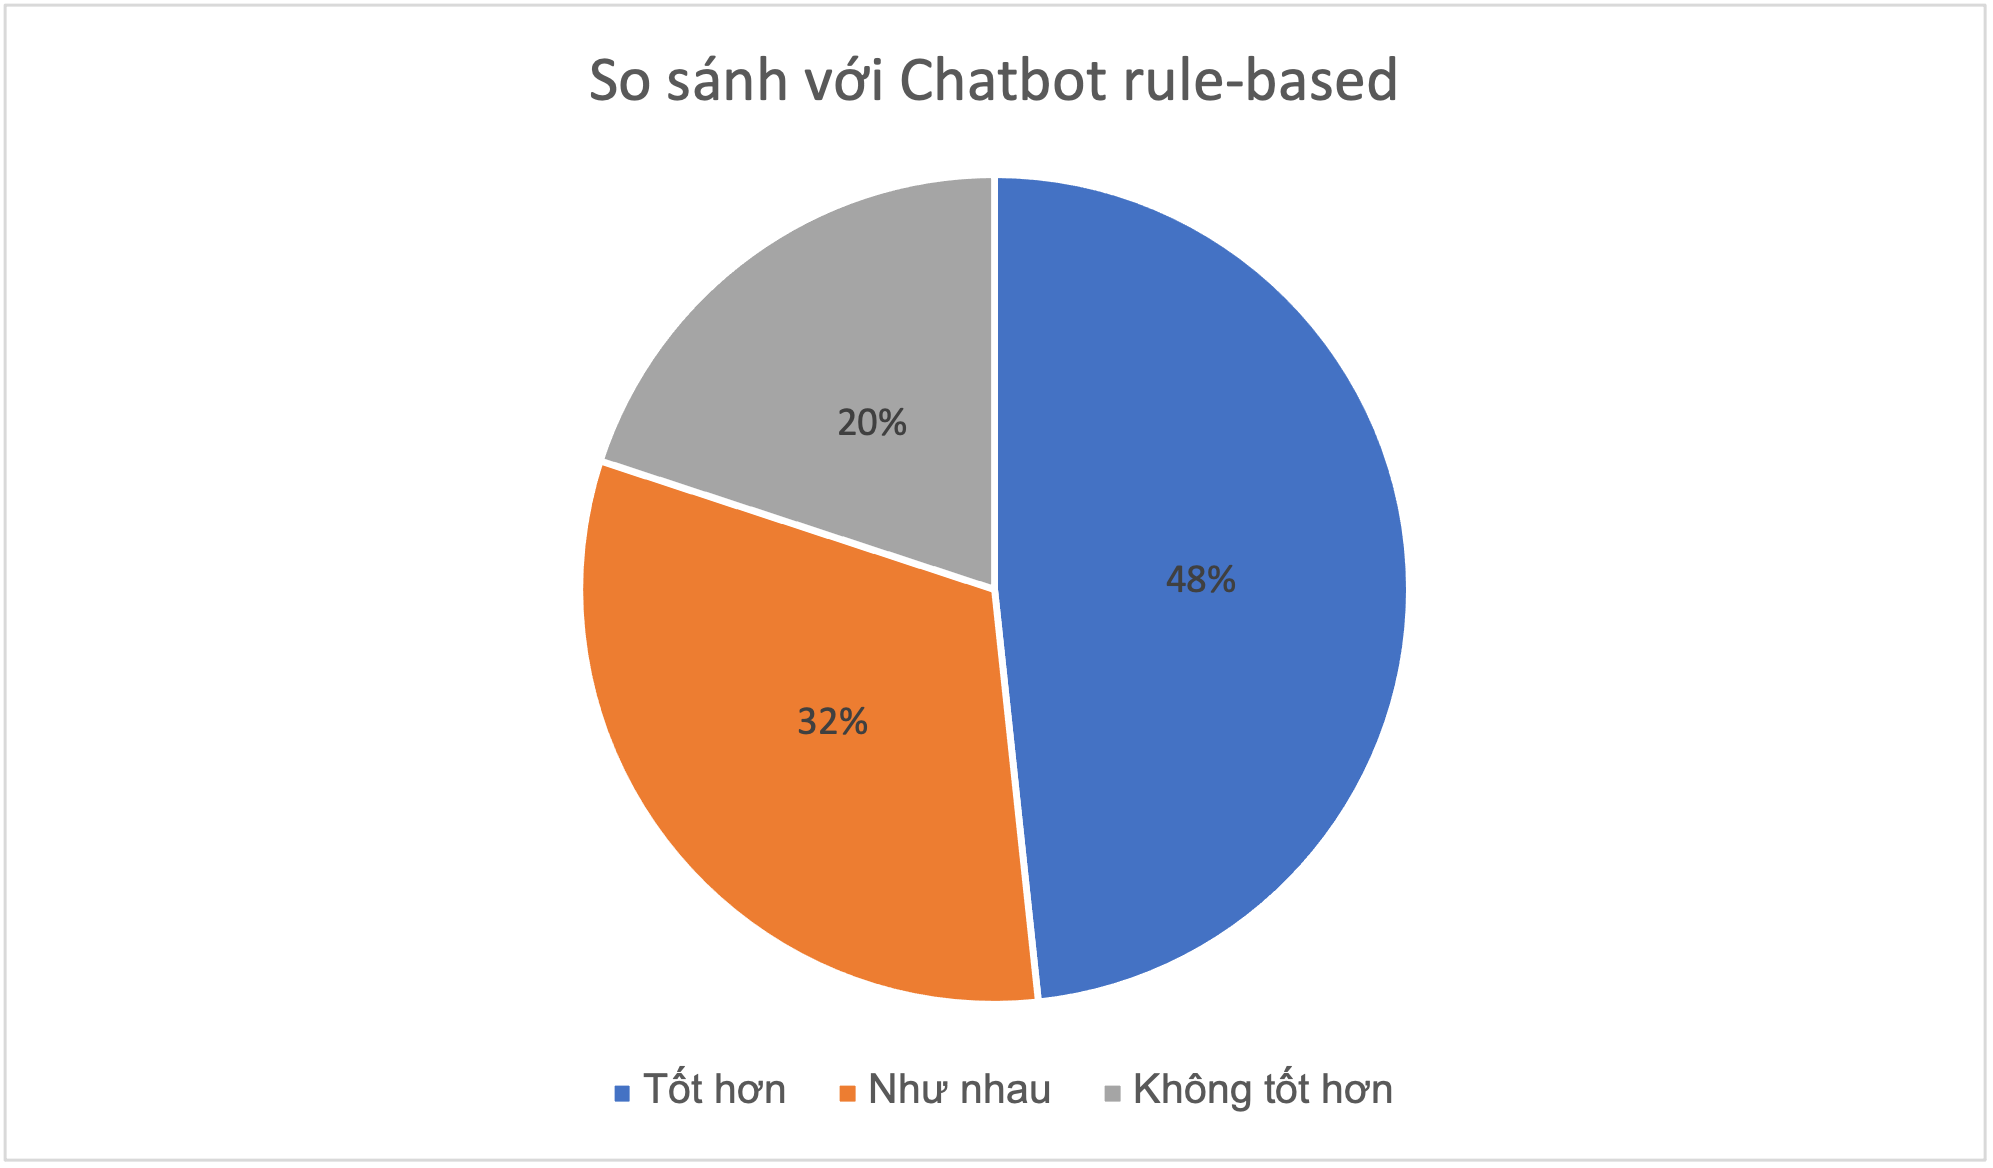
\includegraphics[scale=0.91]{chapter7/img/tieuchi4_2.png}
        \end{center}
        \caption{Kết quả so sánh với Chatbot rule-based}
        \label{fig:tieuchi42}
    \end{figure}
\end{center}

\textbf{Nhận xét:}
Có 90\% nhận xét từ tạm chấp nhận được cho đến thiết thực. Trong đó hơn 50\% là thiết thực. Chỉ có 10\% nhận xét là không thiết thực. Nhận thấy việc gợi ý, cung cấp thông tin về sản phẩm giúp Chatbot có thể thể hiện được khả năng hiểu vấn đề và khả năng cung cấp thông tin có ích cho người dùng.

\subsubsection{So sánh với Chatbot rule-based}
Hình \ref{fig:tieuchi42} mô tả kết quả đánh giá của người dùng khi so sánh tiêu chí tính thiết thực, hữu ích với Chatbot rule-based.\\

\textbf{Nhận xét:}
Có 80\% đánh giá là tốt hơn hoặc tương đương với Chatbot rule-based. Có 20\% là không tốt hơn. Sau khi phân tích cụ thể các kết quả đánh giá không tốt, nhận thấy Chatbot rule-based này sẽ liệt kê tất cả thông tin của sản phẩm trong lượt đầu. Việc này thỏa mãn một số người dùng tốt hơn Chatbot khi sử dụng học tăng cường.

\subsubsection{Tiêu chí về tính chính xác của các thông tin mà tác nhân cung cấp}
Hình \ref{fig:tieuchi5} mô tả kết quả đánh giá của người dùng cho tiêu chí tính chính xác của các thông tin mà tác nhân cung cấp.

\begin{center}
    \begin{figure}[h!]
        \begin{center}
         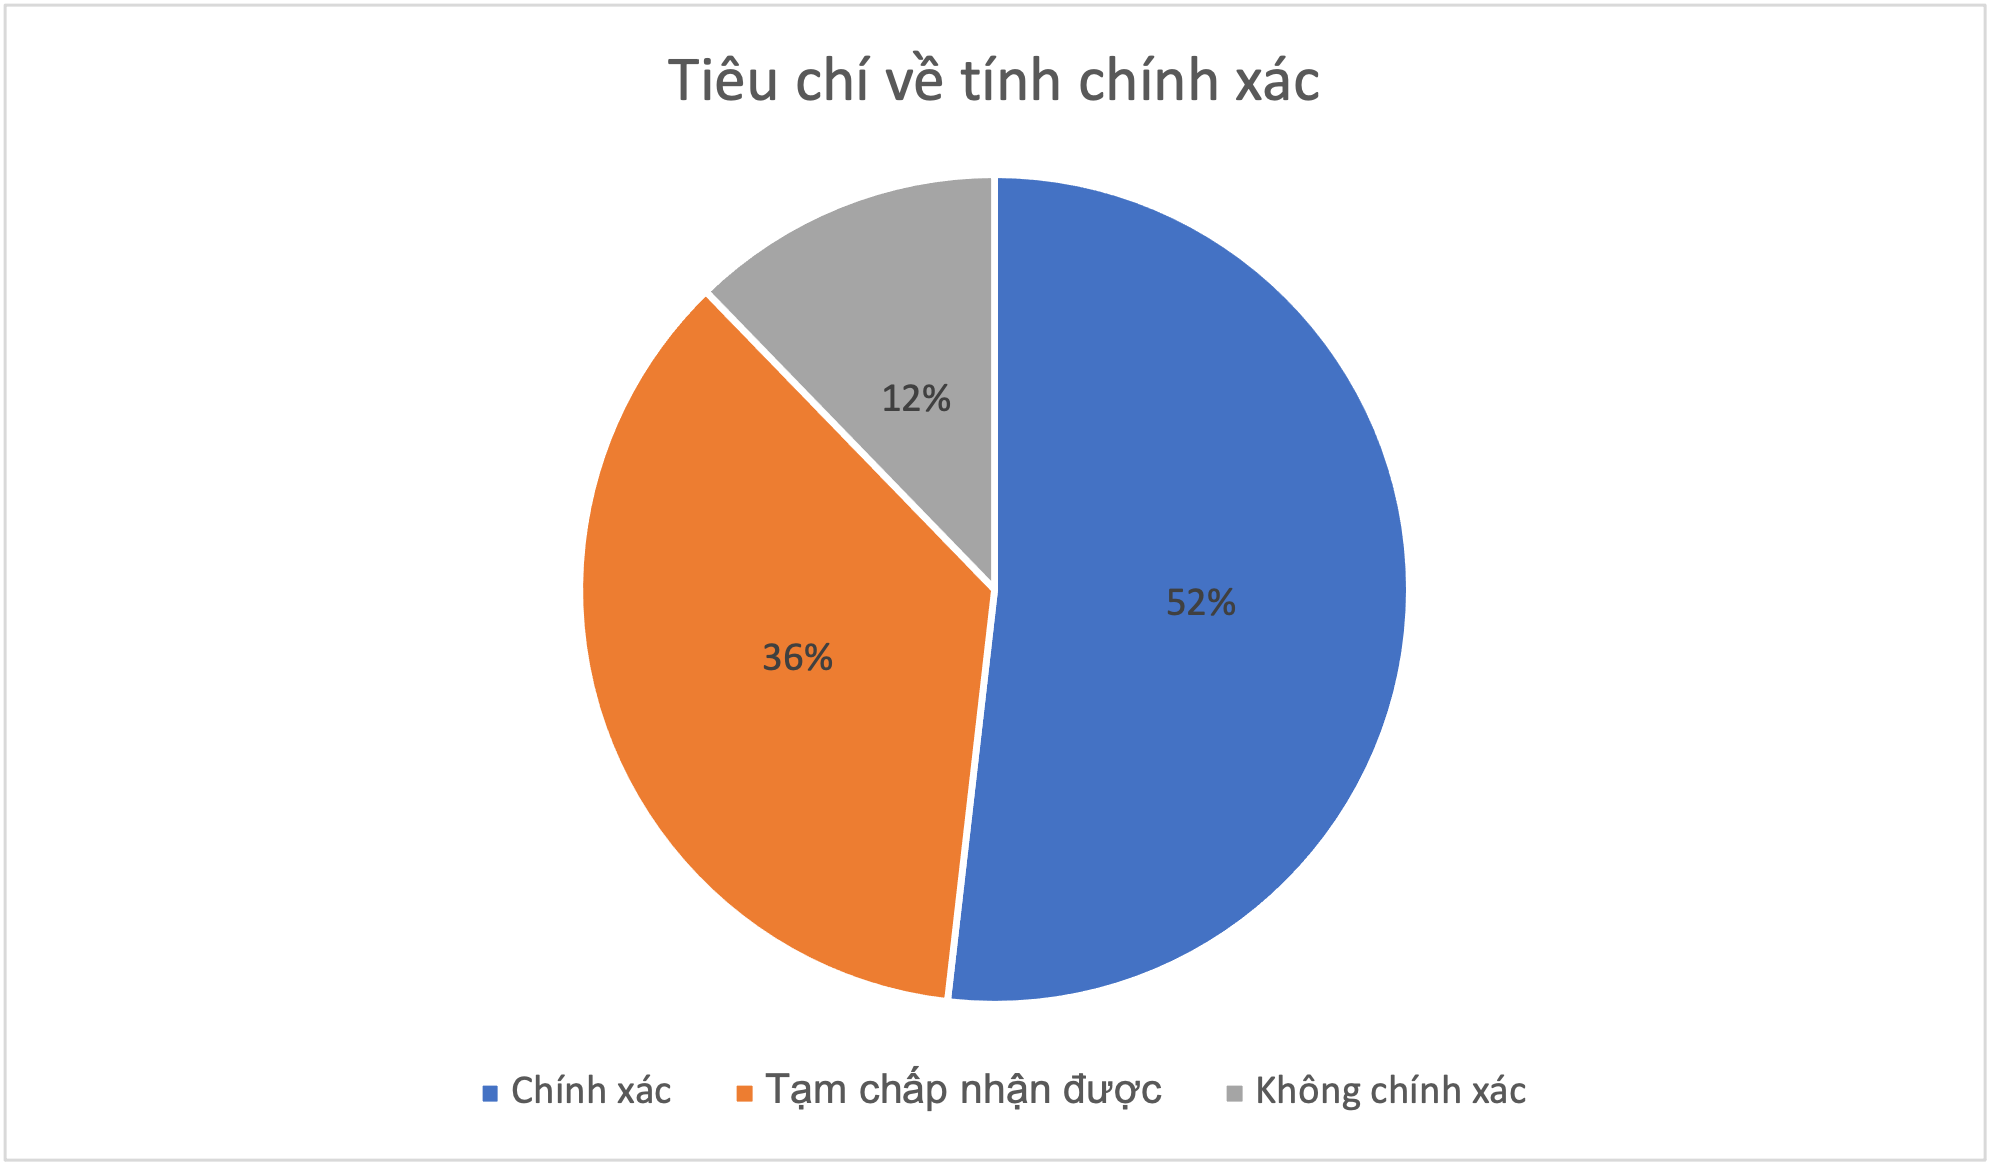
\includegraphics[scale=0.91]{chapter7/img/tieuchi5.png}
        \end{center}
        \caption{Kết quả đánh giá tiêu chí tính chính xác}
        \label{fig:tieuchi5}
    \end{figure}
\end{center}

\textbf{Nhận xét:}
Có 90\% nhận xét từ tạm chấp nhận được cho đến chính xác. Trong đó hơn 50\% là chính xác. Chỉ có 12\% nhận xét là không chính xác. Hiện tại việc xác định thông tin người dùng thắc mắc là đúng hay sai chỉ thực hiện thông qua phương pháp so trùng đơn giản nên việc xác định này cũng còn khá hạn chế.

\subsubsection{Tiêu chí về mức độ đáp ứng nhu cầu tư vấn sản phẩm nói chung}
Hình \ref{fig:tieuchi6} mô tả kết quả đánh giá của người dùng cho tiêu chí về mức độ đáp ứng nhu cầu tư vấn sản phẩm nói chung.

\begin{center}
    \begin{figure}[h!]
        \begin{center}
         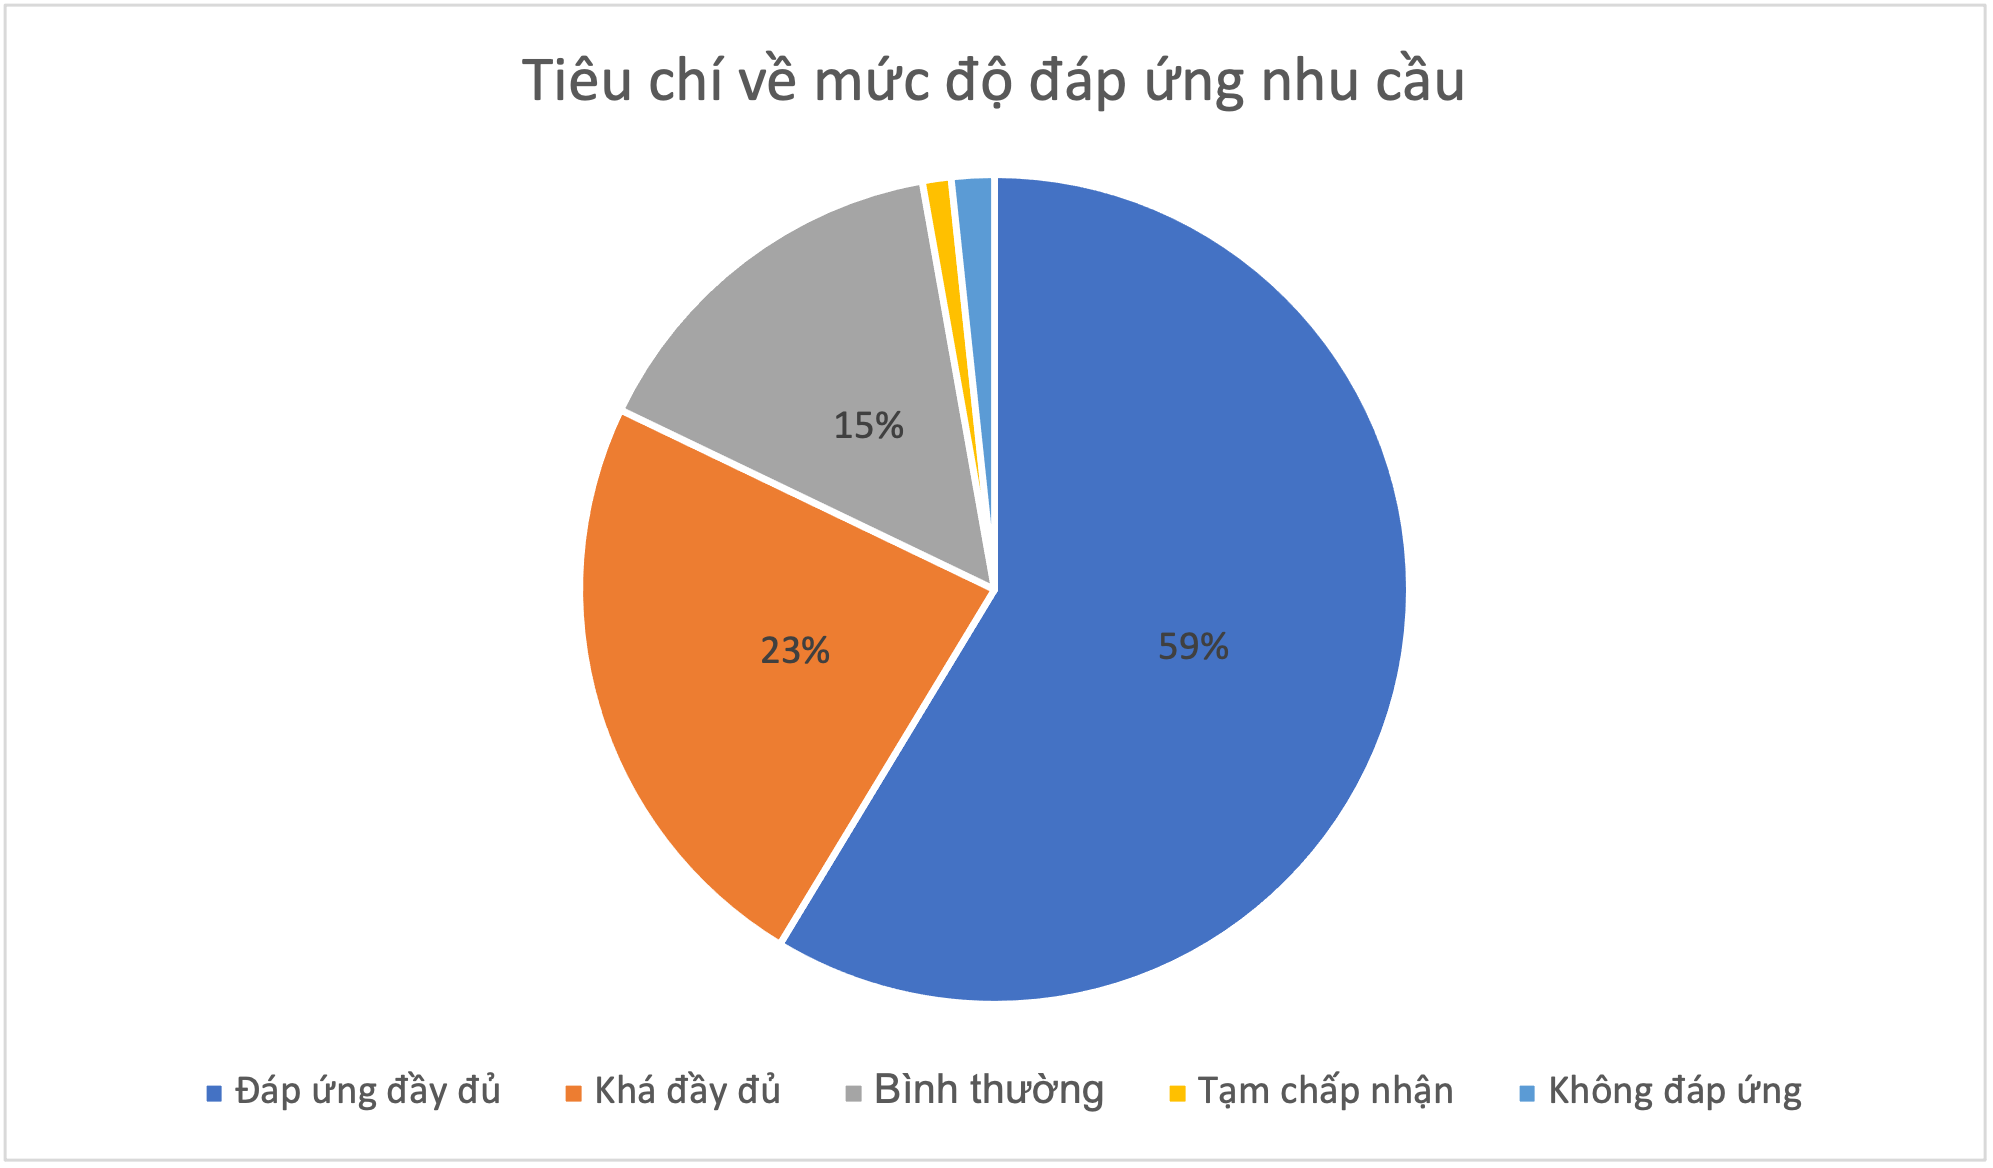
\includegraphics[scale=0.91]{chapter7/img/tieuchi6.png}
        \end{center}
        \caption{Kết quả đánh giá tiêu chí mức độ đáp ứng nhu cầu}
        \label{fig:tieuchi6}
    \end{figure}
\end{center}

\begin{center}
    \begin{figure}[h!]
        \begin{center}
         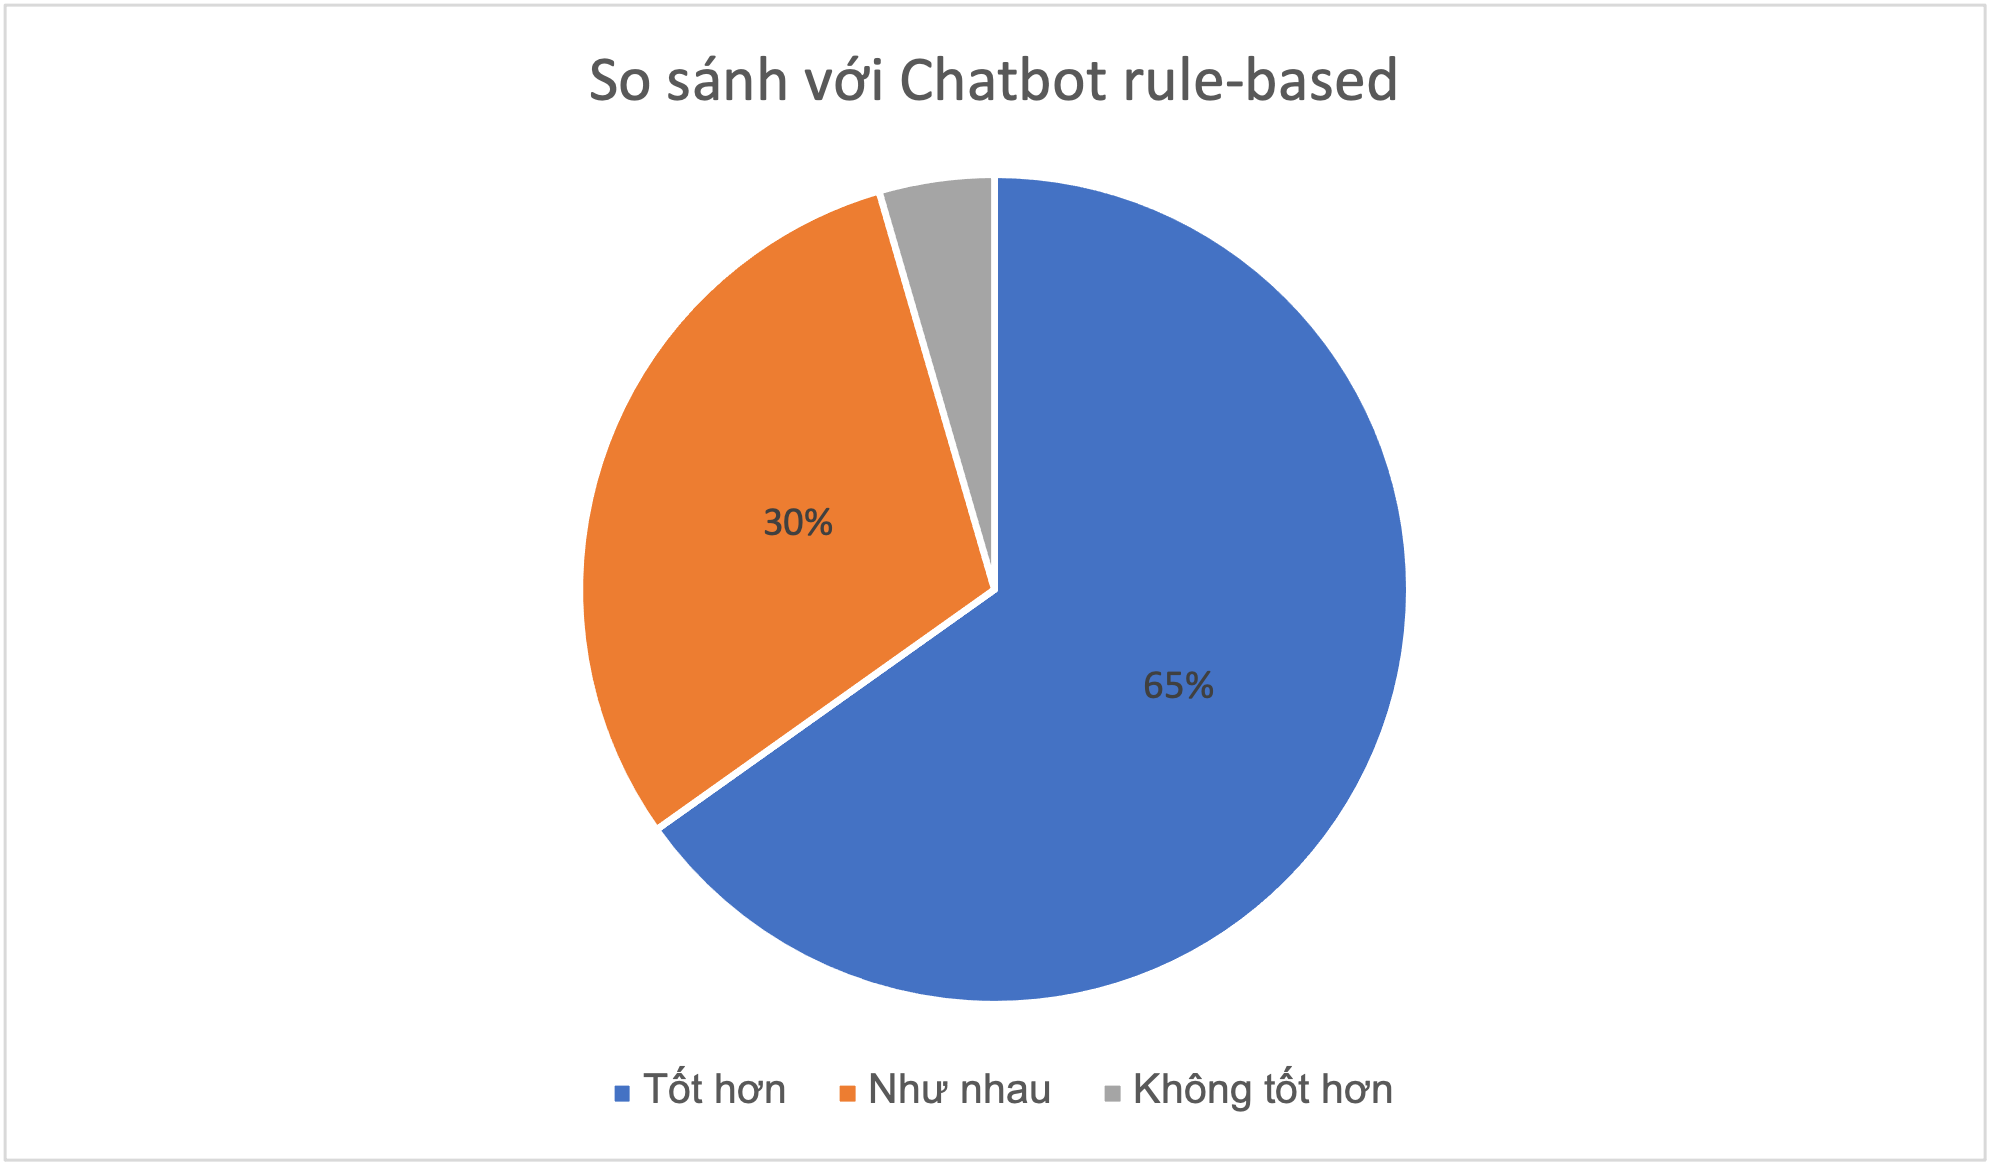
\includegraphics[scale=0.91]{chapter7/img/tieuchi6_2.png}
        \end{center}
        \caption{Kết quả so sánh với Chatbot rule-based}
        \label{fig:tieuchi62}
    \end{figure}
\end{center}

\textbf{Nhận xét:}
Có 97\% nhận xét từ bình thường cho đến đáp ứng đầy đủ. Trong đó hơn 50\% là đáp ứng đầy đủ. Kết quả đánh giá như vậy là rất cao. Biểu thị Chatbot được huấn luyện đáp ứng rất tốt các yêu cầu của người dùng. Tuy nhiên, ta vẫn có 2\% nhận xét là không đáp ứng. Như đã đề cập về những hạn chế ở những mục trước cũng như vấn đề về dữ liệu thực tế chưa thực sự đầy đủ dẫn đến việc thông tin người dùng cần vẫn chưa được cung cấp đầy đủ và chính xác.

\subsubsection{So sánh với Chatbot rule-based}
Hình \ref{fig:tieuchi62} mô tả kết quả đánh giá của người dùng khi so sánh tiêu chí mức độ đáp ứng nhu cầu với Chatbot rule-based.\\

\textbf{Nhận xét:}
Có 95\% đánh giá là tốt hơn hoặc tương đương với Chatbot rule-based. Chỉ có 5\% là không tốt hơn. Tương tự với nguyên nhân được đề cập ở các tiêu chí trước, Chatbot rule-based này sẽ liệt kê tất cả thông tin của sản phẩm trong lượt đầu. Việc này thỏa mãn một số người dùng tốt hơn Chatbot khi sử dụng học tăng cường.

\subsubsection{Tiêu chí về mức độ giao tiếp tự nhiên trong suốt cuộc hội thoại}
Hình \ref{fig:tieuchi7} mô tả kết quả đánh giá của người dùng cho tiêu chí về mức độ giao tiếp tự nhiên trong suốt cuộc hội thoại.

\begin{center}
    \begin{figure}[h!]
        \begin{center}
         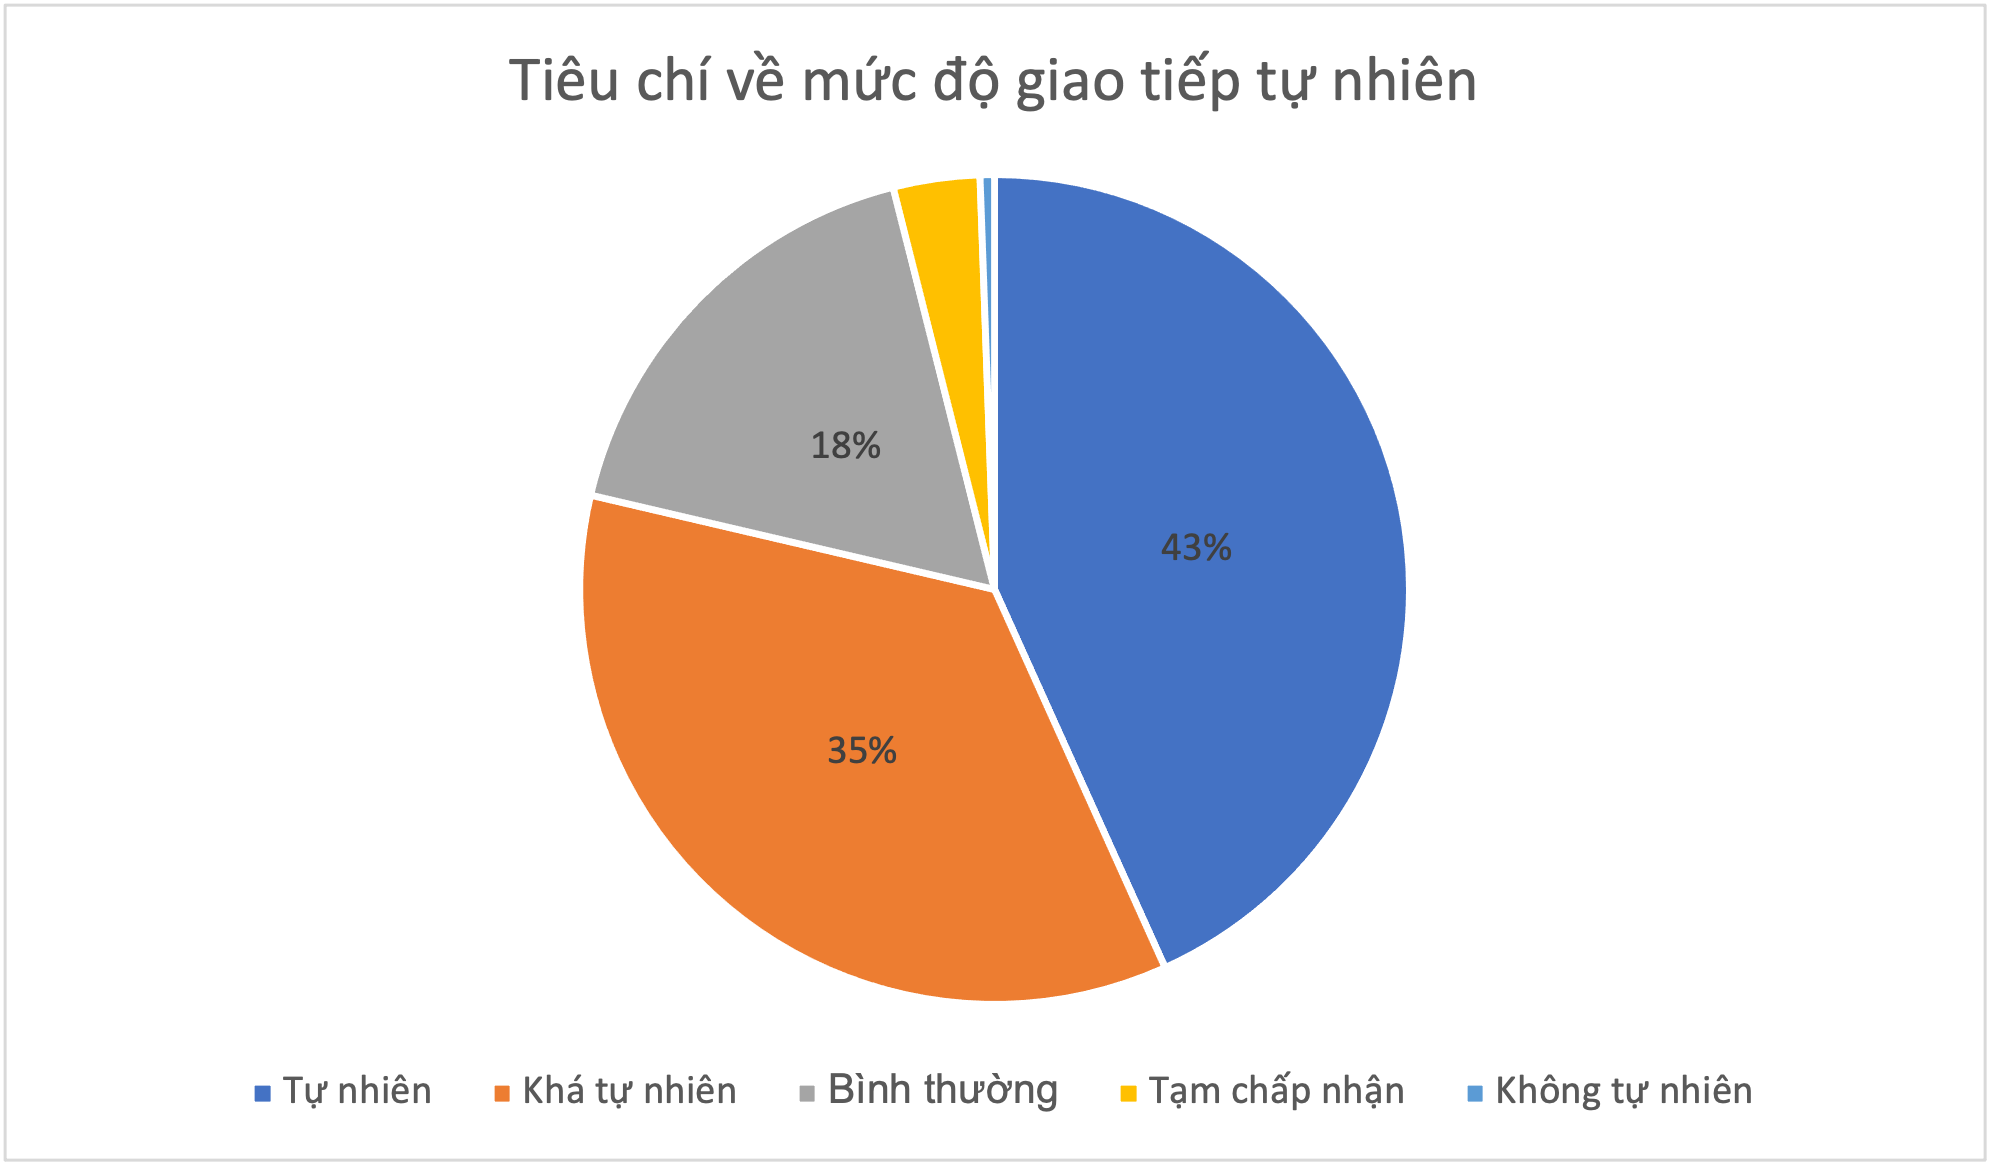
\includegraphics[scale=0.91]{chapter7/img/tieuchi7.png}
        \end{center}
        \caption{Kết quả đánh giá tiêu chí mức độ giao tiếp tự nhiên}
        \label{fig:tieuchi7}
    \end{figure}
\end{center}

\textbf{Nhận xét:}
Có 96\% nhận xét từ bình thường cho đến tự nhiên. Trong đó gần 50\% là tự nhiên. Chỉ có 1\% là không tự nhiên. Kết quả đánh giá như vậy là rất cao. Biểu thị Chatbot được huấn luyện giao tiếp với người dùng một cách tự nhiên phù hợp.

\subsubsection{So sánh với Chatbot rule-based}
Hình \ref{fig:tieuchi72} mô tả kết quả đánh giá của người dùng khi so sánh tiêu chí mức độ giao tiếp tự nhiên với Chatbot rule-based.

\begin{center}
    \begin{figure}[h!]
        \begin{center}
         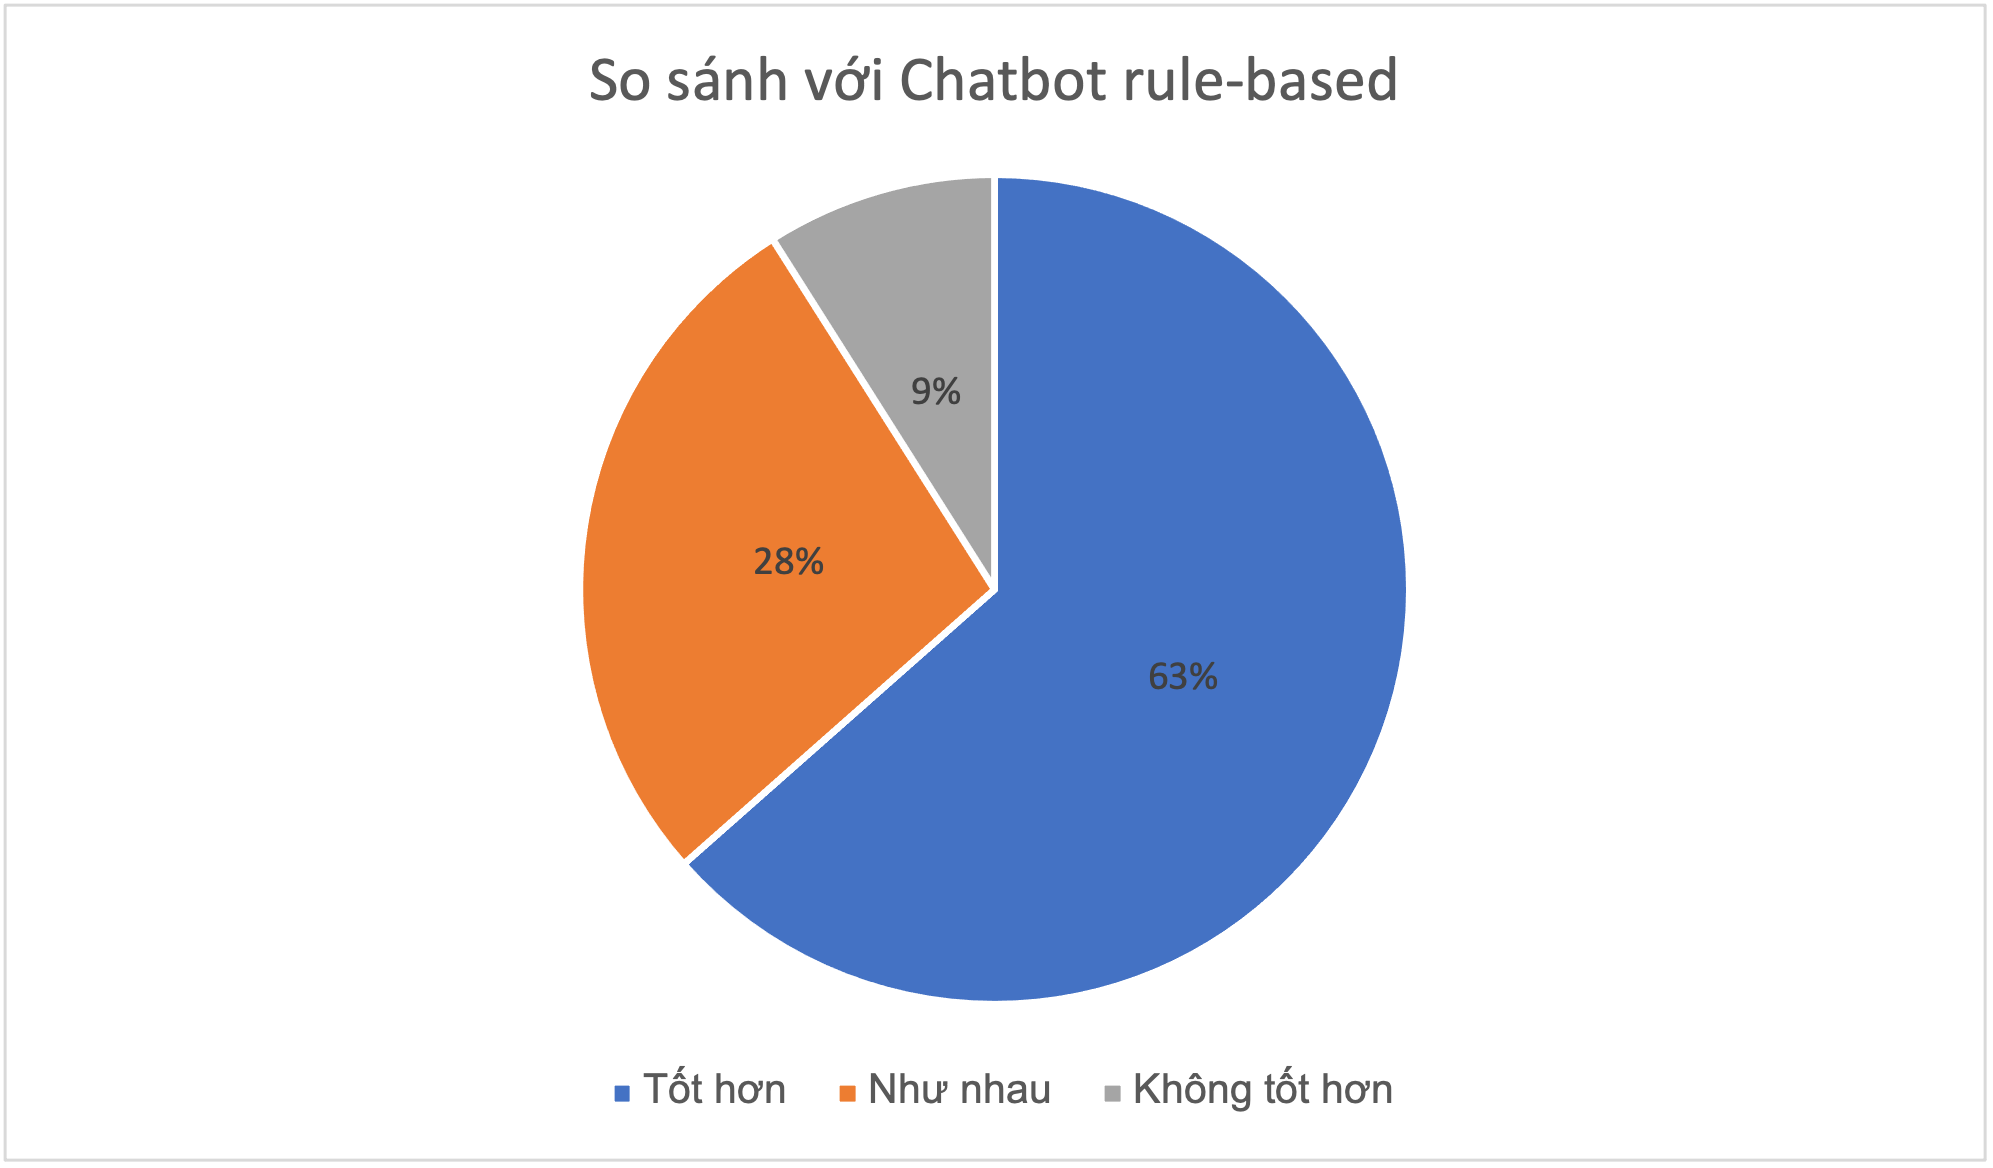
\includegraphics[scale=0.91]{chapter7/img/tieuchi7_2.png}
        \end{center}
        \caption{Kết quả so sánh với Chatbot rule-based}
        \label{fig:tieuchi72}
    \end{figure}
\end{center}

\textbf{Nhận xét:}
Có hơn 90\% đánh giá là tốt hơn hoặc tương đương với Chatbot rule-based. Chỉ có 9\% là không tốt hơn. Yếu tố tự nhiên được đánh giá tùy vào cảm tính của người dùng. Một phần có thể do bộ sinh phản hồi chưa được tốt.

\subsubsection{Đánh giá tổng quan của người dùng}
Hình \ref{fig:tieuchi8} mô tả kết quả đánh giá tổng quan của người dùng trên thang đánh giá 5 sao.

\begin{center}
    \begin{figure}[h!]
        \begin{center}
         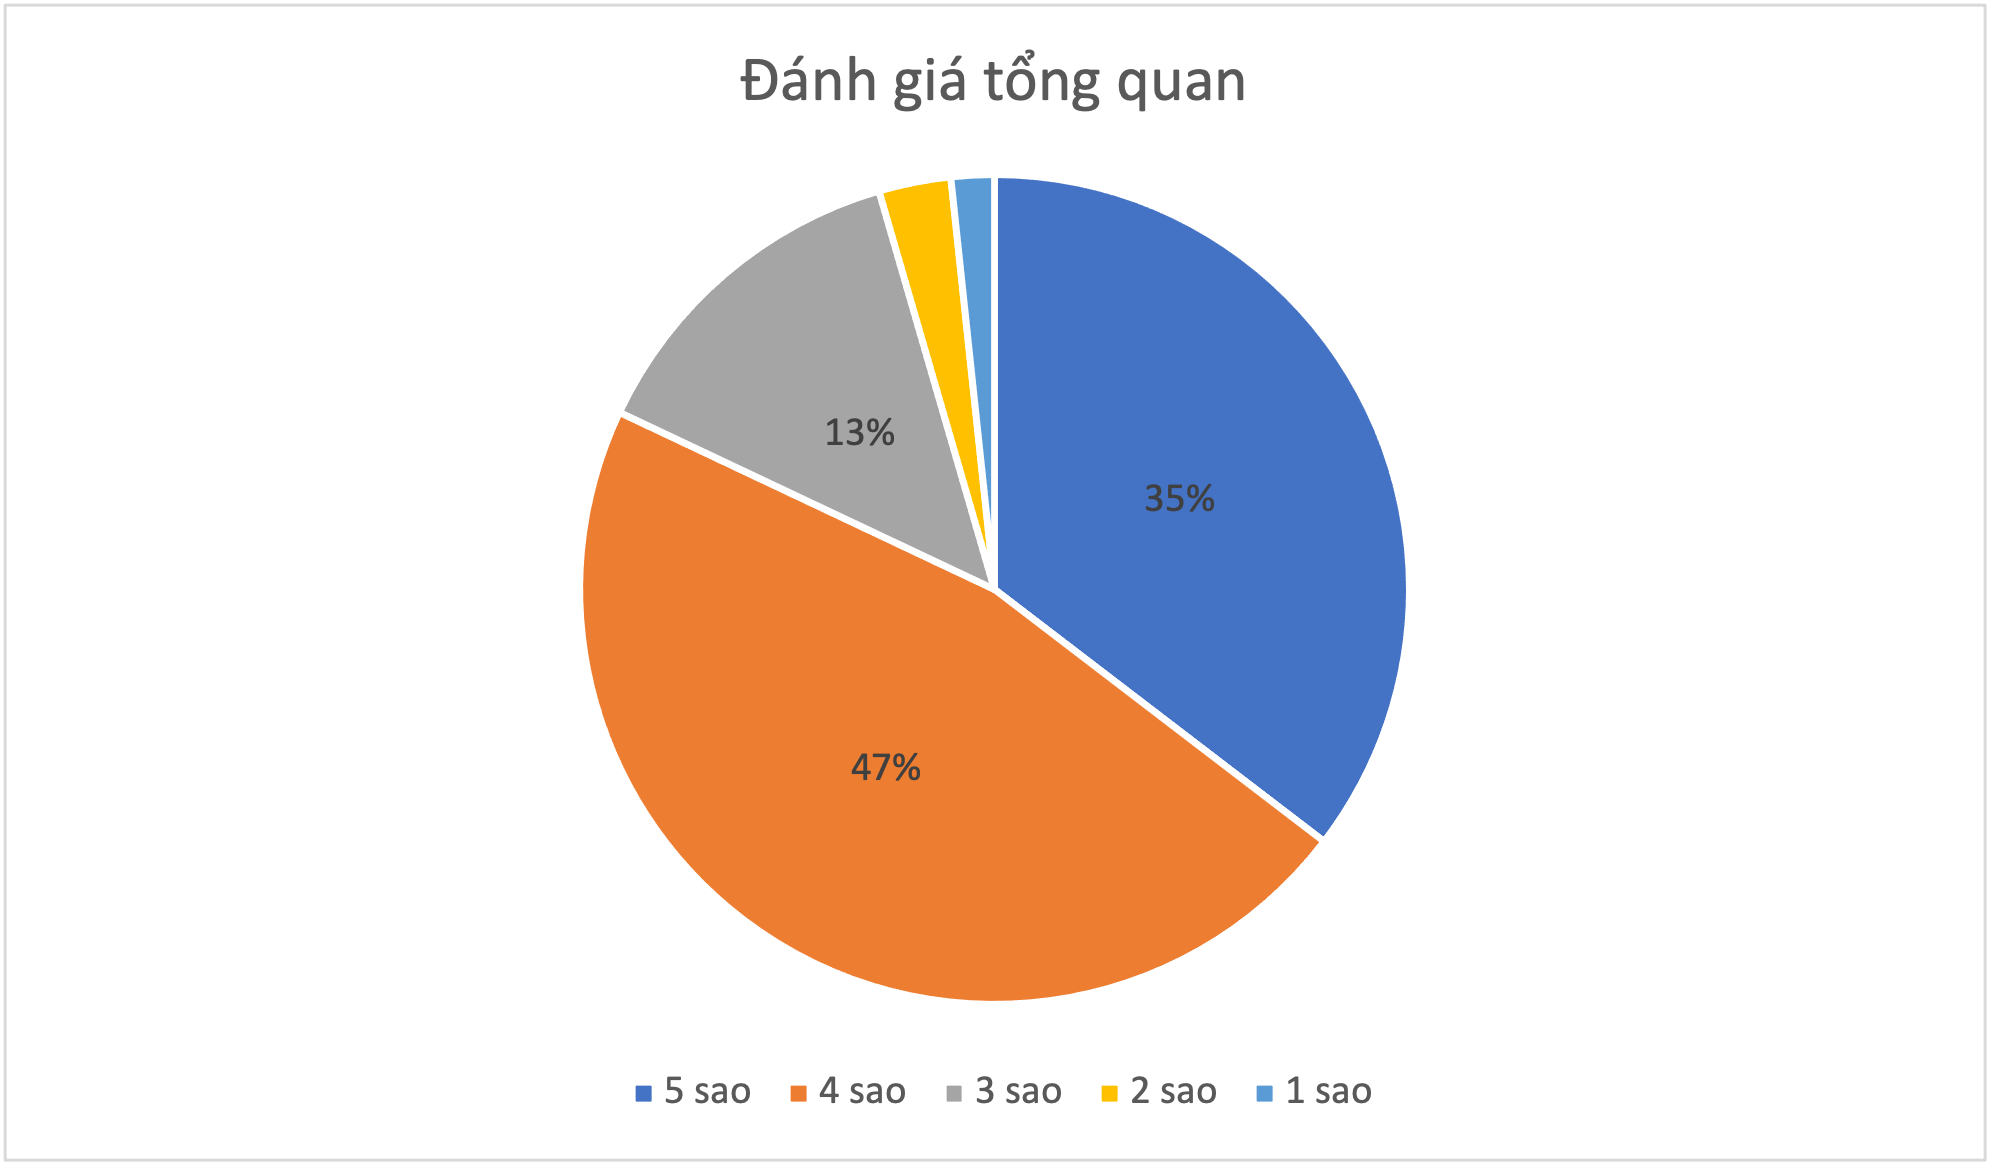
\includegraphics[scale=0.91]{chapter7/img/tieuchi8.png}
        \end{center}
        \caption{Kết quả đánh giá tổng quan của người dùng}
        \label{fig:tieuchi8}
    \end{figure}
\end{center}

\textbf{Nhận xét:}
Kết quả cho thấy có 95\% người dùng đánh giá từ 3 sao trở lên. Xét trên thang điểm 5 sao, Chatbot đạt 4.1 sao.

\section{Kiểm thử ứng dụng Chatbot}
Kiểm thử hệ thống thuộc loại kiểm thử hộp đen (black box). Kiểm thử hệ thống là kiểm tra được thực hiện trên một hệ thống tích hợp hoàn chỉnh để đánh giá sự tuân thủ của hệ thống với các yêu cầu đã chỉ định của nó. Nội dung kiểm thử và tiêu chí đánh giá được mô tả cụ thể sau đây.

\subsection{Kiểm thử giao diện}
Nội dung kiểm thử được mô tả cụ thể ở bảng \ref{tab:uitest}.

\begin{table}[!ht]
\caption{Đặc tả kiểm thử giao diện Chatbot}
\centering
\begin{tabular}{|p{0.8cm}|p{3.2cm}|p{3.2cm}|p{3.6cm}|p{1.8cm}|}
\hline
\centering\textbf{STT} & 
\centering\textbf{Chức năng} & 
\parbox[t]{3.2cm}{\centering\textbf{Nội dung \\kiểm thử}} &
\centering\textbf{Kết quả mong đợi} & 
\parbox[t]{1.8cm}{\centering\textbf{Kết quả \\kiểm thử}} \\ [3ex] % inserts table %heading
\hline
\centering 1 & 
Giao diện Chatbot với các nút bấm chức năng, ô lựa chọn, khung hội thoại và toàn bộ tin nhắn của người dùng và tác nhân cho tới thời điểm hiện tại & 
\parbox[t]{3.2cm}{Bước 1: Truy cập vào ứng dụng Chatbot \\ Bước 2: Thực hiện thao tác trên các nút bấm chức năng} &
Giao diện Chatbot hiển thị đầy đủ các nút bấm, ô lựa chọn, khung hội thoại và toàn bộ tin nhắn của người dùng và tác nhân cho tới thời điểm hiện tại, Kết quả minh họa như hình \ref{fig:testtool} & 
\parbox[t]{1.8cm}{\centering PASS} \\
\hline
\centering 2 & 
Giao diện Chatbot với kích thước trên các thiết bị có độ phân giải và kích thước khác nhau & 
\parbox[t]{3.2cm}{Bước 1: Truy cập vào ứng dụng Chatbot với các trình duyệt khác nhau \\ Bước 2: Thu nhỏ hoặc phóng lớn cửa sổ} &
Giao diện Chatbot giữ nguyên kích thước trên các thiết bị có độ phân giải và kích thước khác nhau, không bị khuất, bị mất nội dung & 
\parbox[t]{1.8cm}{\centering PASS} \\
\hline
\centering 3 & 
Các hiệu ứng hành động trên giao diện Chatbot & 
\parbox[t]{3.2cm}{Bước 1: Truy cập vào ứng dụng Chatbot \\ Bước 2: Thực hiện thao tác trên ứng dụng, quan sát các thay đổi trên giao diện} &
Các hiệu ứng hành động trên giao diện Chatbot hiển thị mượt mà, không gặp hiện tượng giật, đứng khi sử dụng & 
\parbox[t]{1.8cm}{\centering PASS} \\
\hline
\end{tabular}
\label{tab:uitest}
\end{table}

\clearpage

\begin{center}
    \begin{figure}[h!]
        \begin{center}
         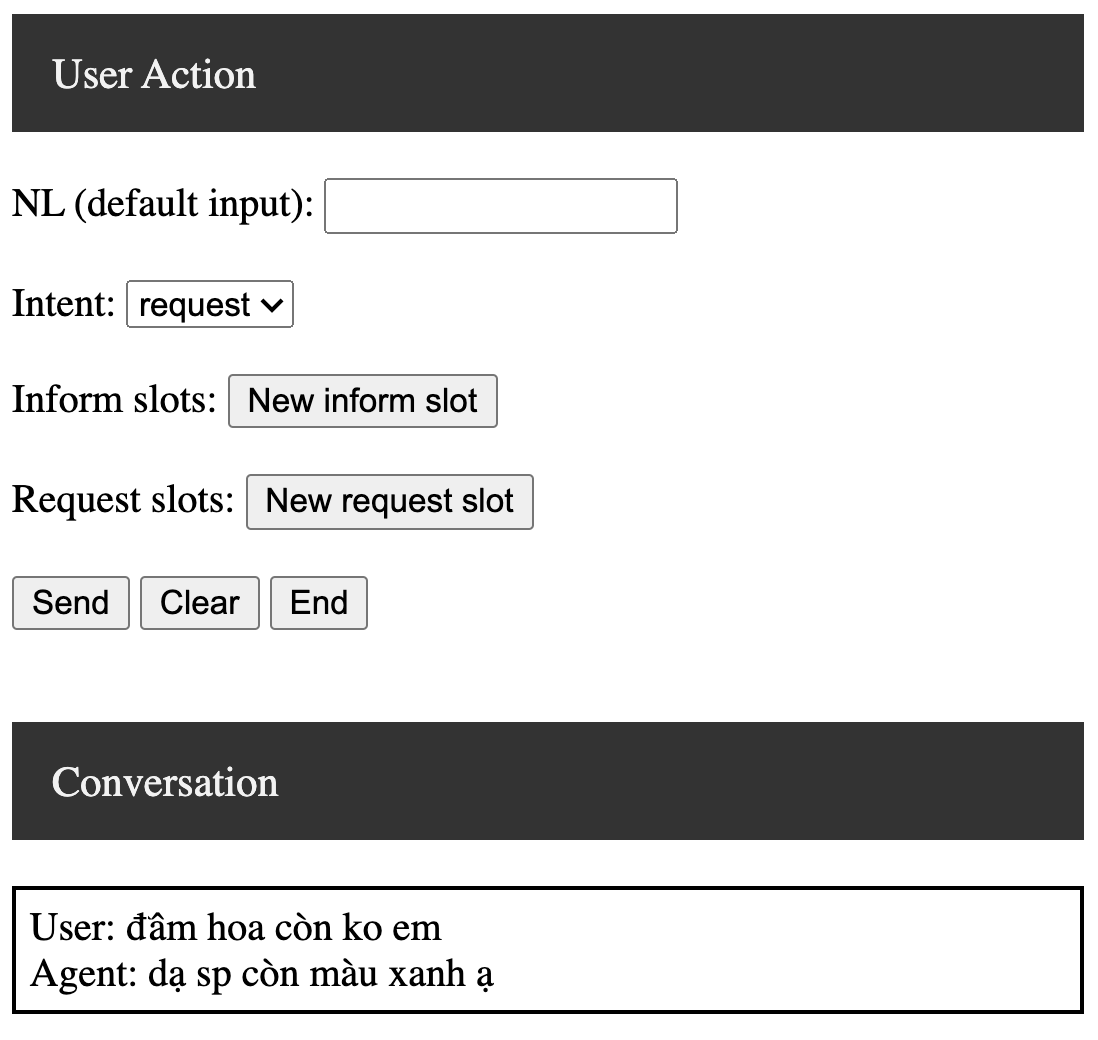
\includegraphics[scale=0.6]{chapter7/img/test_tool.png}
        \end{center}
        \caption{Giao diện của Chatbot}
        \label{fig:testtool}
    \end{figure}
\end{center}

\subsection{Kiểm thử chức năng}
Nội dung kiểm thử được mô tả cụ thể ở bảng \ref{tab:functiontest}.

\begin{table}[!ht]
\caption{Đặc tả kiểm thử chức năng Chatbot}
\centering
\begin{tabular}{|p{0.8cm}|p{2cm}|p{4.4cm}|p{3.6cm}|p{1.8cm}|}
\hline
\centering\textbf{STT} & 
\centering\textbf{Chức năng} & 
\centering\textbf{Nội dung kiểm thử} & 
\centering\textbf{Kết quả mong đợi} & 
\parbox[t]{1.8cm}{\centering\textbf{Kết quả \\kiểm thử}} \\ [3ex] % inserts table %heading
\hline
\centering 1 & 
Gửi hành động người dùng & 
\parbox[t]{4.4cm}{Bước 1: Nhập câu thoại hoặc lựa chọn hành động thông qua các ô lựa chọn \\ Bước 2: Gửi hành động} &
Chatbot nhận được hành động của người dùng, không sai lệch, thiếu thông tin & 
\parbox[t]{1.8cm}{\centering PASS} \\
\hline
\centering 2 & 
Xóa hành động người dùng & 
\parbox[t]{4.4cm}{Bước 1: Nhập câu thoại hoặc lựa chọn hành động thông qua các ô lựa chọn \\ Bước 2: Xóa hành động} &
Chatbot xóa hành động đang nhập hiện tại của người dùng. Trạng thái hội thoại không thay đổi & 
\parbox[t]{1.8cm}{\centering PASS} \\
\hline
\centering 3 & 
Phản hồi người dùng & 
\parbox[t]{4.4cm}{Bước 1: Nhập câu thoại hoặc lựa chọn hành động thông qua các ô lựa chọn \\ Bước 2: Gửi hành động} &
Chatbot có phản hồi với mỗi tin nhắn của người dùng và hiển thị câu phản hồi trên khung hội thoại & 
\parbox[t]{1.8cm}{\centering PASS} \\
\hline
\centering 4 & 
Kết thúc hội thoại & 
\parbox[t]{4.4cm}{Bước 1: Nhập câu thoại hoặc lựa chọn hành động thông qua các ô lựa chọn \\ Bước 2: Gửi hành động \\ Bước 3: Nhấn nút kết thúc hội thoại} &
Chatbot xóa toàn bộ nội dung hội thoại, đồng thời thiết lập lại trạng thái hội thoại & 
\parbox[t]{1.8cm}{\centering PASS} \\
\hline
\end{tabular}
\label{tab:functiontest}
\end{table}

% \subsection{Kiểm thử đơn vị}

% \subsubsection{Bộ truy vấn cơ sở dữ liệu}

% \subsubsection{Bộ xử lý phản hồi người dùng}

% \subsubsection{Bộ quản lý trạng thái hội thoại}

% \subsubsection{Bộ sinh phản hồi}

% \subsubsection{Bộ sinh câu phản hồi}

% \clearpage 

\chapter{Tổng kết}

Trong chương này, tổng kết những kết quả đạt được trong Luận văn này, một số mặt hạn chế của đề tài và hướng phát triển trong tương lai.

\section{Các kết quả đạt được}
Những công việc đã đạt được:

\begin{itemize}
    \item Tìm kiếm và thu thập dữ liệu phù hợp với nội dung đề tài. 
    \item Tổ chức đánh nhãn với sự giúp đỡ của các bạn cộng tác viên.
    \item Khảo sát nhu cầu của người dùng và cửa hàng cụ thể trong tư vấn thông tin sản phẩm, từ đó xây dựng các kịch bản, nhiệm vụ cho Chatbot.
    \item Tiến hành huấn luyện mô hình học tăng cường để có thể đưa ra quyết định cho mỗi hành động khi giao tiếp với người dùng cũng như truy vấn dữ liệu chính xác để trả về đúng thông tin người dùng mong muốn.
    \item Xây dựng bộ sinh câu phản hồi của Chatbot với ngôn từ tự nhiên tạo cảm giác thoải mái cho người dùng.
    \item Tổ chức đánh giá chất lượng hệ thống và thu được phản hồi tích cực từ người dùng.
\end{itemize}

\section{Các hạn chế}
Một số hạn chế của hệ thống:

\begin{itemize}
    \item Quá trình chuẩn hóa dữ liệu còn nhiều thiếu sót, việc này phụ thuộc vào bộ từ điển dữ liệu. Từ đó, phát sinh các trường hợp không nhận diện được đúng đắn thông tin người dùng cung cấp. 
    \item Mỗi một cuộc hội thoại diễn ra, mô hình này chỉ tư vấn và chốt được đơn hàng cho một loại sản phẩm. Việc này dễ thấy thông qua định dạng hành động của người dùng lẫn tác nhân. Các thông tin phụ thuộc lẫn nhau như tên sản phẩm đi kèm với kích cỡ hay màu sắc, ... không có cấu trúc phân cấp.
\end{itemize}

\section{Định hướng trong tương lai}
Một số cải tiến cho hệ thống này như sau:

\begin{itemize}
    \item Cập nhật thêm các ý định của người dùng để quá trình tư vấn phong phú, hỗ trợ tốt hơn cho người dùng.
    \item Tìm cách sử dụng các mô hình học máy hoặc phương án khác hỗ trợ cho việc chuẩn hóa tốt hơn.
    \item Tìm cách sửa đổi định dạng hành động cũng như bộ quản lý trạng thái hội thoại, cách thức quản lý thông tin được thông báo hoặc yêu cầu tương ứng với nhau.
    \item Mô hình tư vấn này có thể được tích hợp trong nhiều hệ thống Chatbot khác.
\end{itemize}


%bibliography{refs}{}
%bibliographystyle{plain}
%-	Danh mục TL tham khảo
%-	Phụ lục (nếu có)
\renewcommand\bibname{TÀI LIỆU THAM KHẢO}

\begin{thebibliography}{}

% reference in chapter 1
\bibitem{decisiontreesinpythonwithscikitlearn} 
Scott Robinson, Decision Trees in Python with Scikit-Learn
\\\url{https://stackabuse.com/decision-trees-in-python-with-scikit-learn/}

% reference in chapter 3
\bibitem{userguide}
Scikit-learn, User Guide
\\\url{https://scikit-learn.org/stable/modules/tree.html#}

% reference in chapter 6
\bibitem{scikitlearn}
Thư Viện Scikit-learn Trong Python Là Gì?
\\\url{https://codelearn.io/sharing/scikit-learn-trong-python-la-gi}

% reference in chapter 7
\bibitem{decisiontreeclassifier}
Scikit-learn, class sklearn.tree.DecisionTreeClassifier
\\\url{https://scikit-learn.org/stable/modules/generated/sklearn.tree.DecisionTreeClassifier.html}

\end{thebibliography}

\cvpage

\end{document}